\documentclass[twoside]{book}

% Packages required by doxygen
\usepackage{fixltx2e}
\usepackage{calc}
\usepackage{doxygen}
\usepackage[export]{adjustbox} % also loads graphicx
\usepackage{graphicx}
\usepackage[utf8]{inputenc}
\usepackage{makeidx}
\usepackage{multicol}
\usepackage{multirow}
\PassOptionsToPackage{warn}{textcomp}
\usepackage{textcomp}
\usepackage[nointegrals]{wasysym}
\usepackage[table]{xcolor}

% Font selection
\usepackage[T1]{fontenc}
\usepackage[scaled=.90]{helvet}
\usepackage{courier}
\usepackage{amssymb}
\usepackage{sectsty}
\renewcommand{\familydefault}{\sfdefault}
\allsectionsfont{%
  \fontseries{bc}\selectfont%
  \color{darkgray}%
}
\renewcommand{\DoxyLabelFont}{%
  \fontseries{bc}\selectfont%
  \color{darkgray}%
}
\newcommand{\+}{\discretionary{\mbox{\scriptsize$\hookleftarrow$}}{}{}}

% Page & text layout
\usepackage{geometry}
\geometry{%
  a4paper,%
  top=2.5cm,%
  bottom=2.5cm,%
  left=2.5cm,%
  right=2.5cm%
}
\tolerance=750
\hfuzz=15pt
\hbadness=750
\setlength{\emergencystretch}{15pt}
\setlength{\parindent}{0cm}
\setlength{\parskip}{0.2cm}
\makeatletter
\renewcommand{\paragraph}{%
  \@startsection{paragraph}{4}{0ex}{-1.0ex}{1.0ex}{%
    \normalfont\normalsize\bfseries\SS@parafont%
  }%
}
\renewcommand{\subparagraph}{%
  \@startsection{subparagraph}{5}{0ex}{-1.0ex}{1.0ex}{%
    \normalfont\normalsize\bfseries\SS@subparafont%
  }%
}
\makeatother

% Headers & footers
\usepackage{fancyhdr}
\pagestyle{fancyplain}
\fancyhead[LE]{\fancyplain{}{\bfseries\thepage}}
\fancyhead[CE]{\fancyplain{}{}}
\fancyhead[RE]{\fancyplain{}{\bfseries\leftmark}}
\fancyhead[LO]{\fancyplain{}{\bfseries\rightmark}}
\fancyhead[CO]{\fancyplain{}{}}
\fancyhead[RO]{\fancyplain{}{\bfseries\thepage}}
\fancyfoot[LE]{\fancyplain{}{}}
\fancyfoot[CE]{\fancyplain{}{}}
\fancyfoot[RE]{\fancyplain{}{\bfseries\scriptsize Generated on Sun Nov 8 2015 23\+:56\+:52 for My Project by Doxygen }}
\fancyfoot[LO]{\fancyplain{}{\bfseries\scriptsize Generated on Sun Nov 8 2015 23\+:56\+:52 for My Project by Doxygen }}
\fancyfoot[CO]{\fancyplain{}{}}
\fancyfoot[RO]{\fancyplain{}{}}
\renewcommand{\footrulewidth}{0.4pt}
\renewcommand{\chaptermark}[1]{%
  \markboth{#1}{}%
}
\renewcommand{\sectionmark}[1]{%
  \markright{\thesection\ #1}%
}

% Indices & bibliography
\usepackage{natbib}
\usepackage[titles]{tocloft}
\setcounter{tocdepth}{3}
\setcounter{secnumdepth}{5}
\makeindex

% Hyperlinks (required, but should be loaded last)
\usepackage{ifpdf}
\ifpdf
  \usepackage[pdftex,pagebackref=true]{hyperref}
\else
  \usepackage[ps2pdf,pagebackref=true]{hyperref}
\fi
\hypersetup{%
  colorlinks=true,%
  linkcolor=blue,%
  citecolor=blue,%
  unicode%
}

% Custom commands
\newcommand{\clearemptydoublepage}{%
  \newpage{\pagestyle{empty}\cleardoublepage}%
}


%===== C O N T E N T S =====

\begin{document}

% Titlepage & ToC
\hypersetup{pageanchor=false,
             bookmarks=true,
             bookmarksnumbered=true,
             pdfencoding=unicode
            }
\pagenumbering{roman}
\begin{titlepage}
\vspace*{7cm}
\begin{center}%
{\Large My Project }\\
\vspace*{1cm}
{\large Generated by Doxygen 1.8.10}\\
\vspace*{0.5cm}
{\small Sun Nov 8 2015 23:56:52}\\
\end{center}
\end{titlepage}
\clearemptydoublepage
\tableofcontents
\clearemptydoublepage
\pagenumbering{arabic}
\hypersetup{pageanchor=true}

%--- Begin generated contents ---
\chapter{Hierarchical Index}
\section{Class Hierarchy}
This inheritance list is sorted roughly, but not completely, alphabetically\+:\begin{DoxyCompactList}
\item \contentsline{section}{Atleta}{\pageref{class_atleta}}{}
\item \contentsline{section}{Equipa\+:\+:Atleta\+Existe}{\pageref{class_equipa_1_1_atleta_existe}}{}
\item \contentsline{section}{Bilhete}{\pageref{class_bilhete}}{}
\item \contentsline{section}{Bilhetes\+Hash}{\pageref{struct_bilhetes_hash}}{}
\item \contentsline{section}{Binary\+Node$<$ Comparable $>$}{\pageref{class_binary_node}}{}
\item \contentsline{section}{Binary\+Node$<$ Prova $>$}{\pageref{class_binary_node}}{}
\item \contentsline{section}{B\+S\+T$<$ Comparable $>$}{\pageref{class_b_s_t}}{}
\item \contentsline{section}{B\+S\+T$<$ Prova $>$}{\pageref{class_b_s_t}}{}
\item \contentsline{section}{B\+S\+T\+Itr\+In$<$ Comparable $>$}{\pageref{class_b_s_t_itr_in}}{}
\item \contentsline{section}{B\+S\+T\+Itr\+Level$<$ Comparable $>$}{\pageref{class_b_s_t_itr_level}}{}
\item \contentsline{section}{B\+S\+T\+Itr\+Post$<$ Comparable $>$}{\pageref{class_b_s_t_itr_post}}{}
\item \contentsline{section}{B\+S\+T\+Itr\+Pre$<$ Comparable $>$}{\pageref{class_b_s_t_itr_pre}}{}
\item \contentsline{section}{Campeonato}{\pageref{class_campeonato}}{}
\item \contentsline{section}{Carater\+Invalido}{\pageref{class_carater_invalido}}{}
\item \contentsline{section}{Compare}{\pageref{class_compare}}{}
\item \contentsline{section}{Data}{\pageref{class_data}}{}
\item \contentsline{section}{Campeonato\+:\+:Data\+Invalida}{\pageref{class_campeonato_1_1_data_invalida}}{}
\item \contentsline{section}{Desporto}{\pageref{class_desporto}}{}
\item \contentsline{section}{Campeonato\+:\+:Desporto\+Existe}{\pageref{class_campeonato_1_1_desporto_existe}}{}
\item \contentsline{section}{Desporto\+:\+:Desporto\+Inexistente}{\pageref{class_desporto_1_1_desporto_inexistente}}{}
\item \contentsline{section}{eqbil}{\pageref{structeqbil}}{}
\item \contentsline{section}{Equipa}{\pageref{class_equipa}}{}
\item \contentsline{section}{Campeonato\+:\+:Equipa\+Existe}{\pageref{class_campeonato_1_1_equipa_existe}}{}
\item \contentsline{section}{Equipa\+:\+:Equipa\+Inexistente}{\pageref{class_equipa_1_1_equipa_inexistente}}{}
\item \contentsline{section}{Ficheiro\+Inexistente}{\pageref{class_ficheiro_inexistente}}{}
\item \contentsline{section}{genero\+Errado}{\pageref{classgenero_errado}}{}
\item \contentsline{section}{Hora}{\pageref{class_hora}}{}
\item \contentsline{section}{Campeonato\+:\+:Hora\+Invalida}{\pageref{class_campeonato_1_1_hora_invalida}}{}
\item \contentsline{section}{Load}{\pageref{struct_load}}{}
\item \contentsline{section}{Load\+Fail}{\pageref{class_load_fail}}{}
\item \contentsline{section}{Load\+Provas\+Fail}{\pageref{class_load_provas_fail}}{}
\begin{DoxyCompactList}
\item \contentsline{section}{Data\+:\+:Data\+Invalida}{\pageref{class_data_1_1_data_invalida}}{}
\item \contentsline{section}{Hora\+:\+:Hora\+Invalida}{\pageref{class_hora_1_1_hora_invalida}}{}
\item \contentsline{section}{Modalidade\+:\+:Modalidade\+Inexistente}{\pageref{class_modalidade_1_1_modalidade_inexistente}}{}
\item \contentsline{section}{Prova\+:\+:Provas\+Simultaneas}{\pageref{class_prova_1_1_provas_simultaneas}}{}
\end{DoxyCompactList}
\item \contentsline{section}{Medalhas}{\pageref{struct_medalhas}}{}
\item \contentsline{section}{Modalidade}{\pageref{class_modalidade}}{}
\item \contentsline{section}{Desporto\+:\+:Modalidade\+Existe}{\pageref{class_desporto_1_1_modalidade_existe}}{}
\item \contentsline{section}{Pontuacao}{\pageref{struct_pontuacao}}{}
\item \contentsline{section}{Prova}{\pageref{class_prova}}{}
\begin{DoxyCompactList}
\item \contentsline{section}{Prova\+Terminada}{\pageref{class_prova_terminada}}{}
\end{DoxyCompactList}
\item \contentsline{section}{Prova\+:\+:Prova\+Inexistente}{\pageref{class_prova_1_1_prova_inexistente}}{}
\end{DoxyCompactList}

\chapter{Class Index}
\section{Class List}
Here are the classes, structs, unions and interfaces with brief descriptions\+:\begin{DoxyCompactList}
\item\contentsline{section}{\hyperlink{class_atleta}{Atleta} }{\pageref{class_atleta}}{}
\item\contentsline{section}{\hyperlink{class_equipa_1_1_atleta_existe}{Equipa\+::\+Atleta\+Existe} }{\pageref{class_equipa_1_1_atleta_existe}}{}
\item\contentsline{section}{\hyperlink{class_bilhete}{Bilhete} }{\pageref{class_bilhete}}{}
\item\contentsline{section}{\hyperlink{struct_bilhetes_hash}{Bilhetes\+Hash} }{\pageref{struct_bilhetes_hash}}{}
\item\contentsline{section}{\hyperlink{class_binary_node}{Binary\+Node$<$ Comparable $>$} }{\pageref{class_binary_node}}{}
\item\contentsline{section}{\hyperlink{class_b_s_t}{B\+S\+T$<$ Comparable $>$} }{\pageref{class_b_s_t}}{}
\item\contentsline{section}{\hyperlink{class_b_s_t_itr_in}{B\+S\+T\+Itr\+In$<$ Comparable $>$} }{\pageref{class_b_s_t_itr_in}}{}
\item\contentsline{section}{\hyperlink{class_b_s_t_itr_level}{B\+S\+T\+Itr\+Level$<$ Comparable $>$} }{\pageref{class_b_s_t_itr_level}}{}
\item\contentsline{section}{\hyperlink{class_b_s_t_itr_post}{B\+S\+T\+Itr\+Post$<$ Comparable $>$} }{\pageref{class_b_s_t_itr_post}}{}
\item\contentsline{section}{\hyperlink{class_b_s_t_itr_pre}{B\+S\+T\+Itr\+Pre$<$ Comparable $>$} }{\pageref{class_b_s_t_itr_pre}}{}
\item\contentsline{section}{\hyperlink{class_campeonato}{Campeonato} }{\pageref{class_campeonato}}{}
\item\contentsline{section}{\hyperlink{class_carater_invalido}{Carater\+Invalido} }{\pageref{class_carater_invalido}}{}
\item\contentsline{section}{\hyperlink{class_compare}{Compare} }{\pageref{class_compare}}{}
\item\contentsline{section}{\hyperlink{class_data}{Data} }{\pageref{class_data}}{}
\item\contentsline{section}{\hyperlink{class_data_1_1_data_invalida}{Data\+::\+Data\+Invalida} }{\pageref{class_data_1_1_data_invalida}}{}
\item\contentsline{section}{\hyperlink{class_campeonato_1_1_data_invalida}{Campeonato\+::\+Data\+Invalida} }{\pageref{class_campeonato_1_1_data_invalida}}{}
\item\contentsline{section}{\hyperlink{class_desporto}{Desporto} }{\pageref{class_desporto}}{}
\item\contentsline{section}{\hyperlink{class_campeonato_1_1_desporto_existe}{Campeonato\+::\+Desporto\+Existe} }{\pageref{class_campeonato_1_1_desporto_existe}}{}
\item\contentsline{section}{\hyperlink{class_desporto_1_1_desporto_inexistente}{Desporto\+::\+Desporto\+Inexistente} }{\pageref{class_desporto_1_1_desporto_inexistente}}{}
\item\contentsline{section}{\hyperlink{structeqbil}{eqbil} }{\pageref{structeqbil}}{}
\item\contentsline{section}{\hyperlink{class_equipa}{Equipa} }{\pageref{class_equipa}}{}
\item\contentsline{section}{\hyperlink{class_campeonato_1_1_equipa_existe}{Campeonato\+::\+Equipa\+Existe} }{\pageref{class_campeonato_1_1_equipa_existe}}{}
\item\contentsline{section}{\hyperlink{class_equipa_1_1_equipa_inexistente}{Equipa\+::\+Equipa\+Inexistente} }{\pageref{class_equipa_1_1_equipa_inexistente}}{}
\item\contentsline{section}{\hyperlink{class_ficheiro_inexistente}{Ficheiro\+Inexistente} }{\pageref{class_ficheiro_inexistente}}{}
\item\contentsline{section}{\hyperlink{classgenero_errado}{genero\+Errado} }{\pageref{classgenero_errado}}{}
\item\contentsline{section}{\hyperlink{class_hora}{Hora} }{\pageref{class_hora}}{}
\item\contentsline{section}{\hyperlink{class_hora_1_1_hora_invalida}{Hora\+::\+Hora\+Invalida} }{\pageref{class_hora_1_1_hora_invalida}}{}
\item\contentsline{section}{\hyperlink{class_campeonato_1_1_hora_invalida}{Campeonato\+::\+Hora\+Invalida} }{\pageref{class_campeonato_1_1_hora_invalida}}{}
\item\contentsline{section}{\hyperlink{struct_load}{Load} }{\pageref{struct_load}}{}
\item\contentsline{section}{\hyperlink{class_load_fail}{Load\+Fail} }{\pageref{class_load_fail}}{}
\item\contentsline{section}{\hyperlink{class_load_provas_fail}{Load\+Provas\+Fail} }{\pageref{class_load_provas_fail}}{}
\item\contentsline{section}{\hyperlink{struct_medalhas}{Medalhas} }{\pageref{struct_medalhas}}{}
\item\contentsline{section}{\hyperlink{class_modalidade}{Modalidade} }{\pageref{class_modalidade}}{}
\item\contentsline{section}{\hyperlink{class_desporto_1_1_modalidade_existe}{Desporto\+::\+Modalidade\+Existe} }{\pageref{class_desporto_1_1_modalidade_existe}}{}
\item\contentsline{section}{\hyperlink{class_modalidade_1_1_modalidade_inexistente}{Modalidade\+::\+Modalidade\+Inexistente} }{\pageref{class_modalidade_1_1_modalidade_inexistente}}{}
\item\contentsline{section}{\hyperlink{struct_pontuacao}{Pontuacao} }{\pageref{struct_pontuacao}}{}
\item\contentsline{section}{\hyperlink{class_prova}{Prova} }{\pageref{class_prova}}{}
\item\contentsline{section}{\hyperlink{class_prova_1_1_prova_inexistente}{Prova\+::\+Prova\+Inexistente} }{\pageref{class_prova_1_1_prova_inexistente}}{}
\item\contentsline{section}{\hyperlink{class_prova_1_1_provas_simultaneas}{Prova\+::\+Provas\+Simultaneas} }{\pageref{class_prova_1_1_provas_simultaneas}}{}
\item\contentsline{section}{\hyperlink{class_prova_terminada}{Prova\+Terminada} }{\pageref{class_prova_terminada}}{}
\end{DoxyCompactList}

\chapter{Class Documentation}
\hypertarget{class_atleta}{}\section{Atleta Class Reference}
\label{class_atleta}\index{Atleta@{Atleta}}


{\ttfamily \#include $<$Equipa.\+h$>$}

\subsection*{Public Member Functions}
\begin{DoxyCompactItemize}
\item 
\hyperlink{class_atleta_a055b02bad1b7615536e583e1f3708ec3}{Atleta} (string n, \hyperlink{class_equipa}{Equipa} $\ast$e, bool g)
\item 
string \hyperlink{class_atleta_a0f5be5cd0b18f224a7a5281216fc1bfd}{get\+Nome} () const 
\item 
\hyperlink{class_equipa}{Equipa} $\ast$ \hyperlink{class_atleta_a5abede47b955764c546dcd78683d4c1e}{get\+Equipa} () const 
\item 
int \hyperlink{class_atleta_ad10e9d537836304fbe44ce3e23533e2d}{get\+Pontos} () const 
\item 
vector$<$ \hyperlink{class_prova}{Prova} $\ast$ $>$ \hyperlink{class_atleta_a4d87755e5d458d4a2c5d53015669ad21}{get\+Provas} () const 
\item 
vector$<$ \hyperlink{class_modalidade}{Modalidade} $\ast$ $>$ \hyperlink{class_atleta_a4e4a08618d388c914705e4552bee3f00}{get\+Modalidades} () const 
\item 
bool \hyperlink{class_atleta_a85f10fa37fcc45860745893c95dc0b34}{get\+Genero} () const 
\item 
void \hyperlink{class_atleta_a8556e86a2cae3eeafb3d97e6c283241f}{set\+Genero} (bool g)
\item 
void \hyperlink{class_atleta_a35fcdb190f9b6b5100fba23cc98e5304}{set\+Nome} (string n)
\item 
void \hyperlink{class_atleta_a410bd5f21959b99444ed4c0f736cdacc}{set\+Equipa} (\hyperlink{class_equipa}{Equipa} \&eq)
\item 
void \hyperlink{class_atleta_ae70dd68db249f3828ee53c15df67a201}{set\+Provas} (vector$<$ \hyperlink{class_prova}{Prova} $\ast$ $>$ p)
\item 
void \hyperlink{class_atleta_adbaffac5f1bf0eedf090cb0a91734bd5}{set\+Modalidades} (vector$<$ \hyperlink{class_modalidade}{Modalidade} $\ast$ $>$ m)
\item 
void \hyperlink{class_atleta_a9af09149a6b3c22ca514154b4a29b7f3}{setpontos} (int p)
\item 
void \hyperlink{class_atleta_a7a4bee73158d8ee13b4812eb96decb61}{adiciona\+Prova} (\hyperlink{class_prova}{Prova} $\ast$p)
\item 
void \hyperlink{class_atleta_a036b7b9cdf087a63e601b4e3a9f5552f}{adiciona\+Modalidade} (\hyperlink{class_modalidade}{Modalidade} $\ast$m)
\item 
void \hyperlink{class_atleta_af143bde354ddd015eeaaf7ea819887fd}{adiciona\+Pontuacao} (int p)
\item 
void \hyperlink{class_atleta_a72dcf8a7a26d47eb5f39e876cb9537bd}{apaga\+Modalidade} (int indice)
\item 
void \hyperlink{class_atleta_aeefa19a643057d8688448aeafadc3dcb}{apaga\+Prova} (int indice)
\item 
void \hyperlink{class_atleta_a24b4c70d5e08a875612c8e234fa4ab44}{menu} ()
\item 
bool \hyperlink{class_atleta_a2c2de5e4a0f9963dd9c1a6507b593aed}{operator==} (const \hyperlink{class_atleta}{Atleta} \&c) const 
\item 
bool \hyperlink{class_atleta_a86b4c8fda3582aab61d9796bc5bdced3}{operator$<$} (const \hyperlink{class_atleta}{Atleta} \&a) const 
\item 
\hyperlink{class_atleta}{Atleta} \& \hyperlink{class_atleta_aea00de3983e444705d4f06702b344413}{operator=} (const \hyperlink{class_atleta}{Atleta} \&a)
\end{DoxyCompactItemize}
\subsection*{Friends}
\begin{DoxyCompactItemize}
\item 
ostream \& \hyperlink{class_atleta_a49ef3d4a229ab0e44df89ff6bf7f0e61}{operator$<$$<$} (ostream \&o, const \hyperlink{class_atleta}{Atleta} \&d)
\end{DoxyCompactItemize}


\subsection{Detailed Description}
Class \hyperlink{class_equipa}{Equipa}

Representa um atleta de uma equipa 

\subsection{Constructor \& Destructor Documentation}
\hypertarget{class_atleta_a055b02bad1b7615536e583e1f3708ec3}{}\index{Atleta@{Atleta}!Atleta@{Atleta}}
\index{Atleta@{Atleta}!Atleta@{Atleta}}
\subsubsection[{Atleta(string n, Equipa $\ast$e, bool g)}]{\setlength{\rightskip}{0pt plus 5cm}Atleta\+::\+Atleta (
\begin{DoxyParamCaption}
\item[{string}]{n, }
\item[{{\bf Equipa} $\ast$}]{e, }
\item[{bool}]{g}
\end{DoxyParamCaption}
)}\label{class_atleta_a055b02bad1b7615536e583e1f3708ec3}
Inicializa os atributos


\begin{DoxyParams}{Parameters}
{\em n} & -\/ nome do atleta \\
\hline
{\em e} & -\/ equipa \\
\hline
{\em g} & -\/ genero (true feminino, false masculino) \\
\hline
\end{DoxyParams}


\subsection{Member Function Documentation}
\hypertarget{class_atleta_a036b7b9cdf087a63e601b4e3a9f5552f}{}\index{Atleta@{Atleta}!adiciona\+Modalidade@{adiciona\+Modalidade}}
\index{adiciona\+Modalidade@{adiciona\+Modalidade}!Atleta@{Atleta}}
\subsubsection[{adiciona\+Modalidade(\+Modalidade $\ast$m)}]{\setlength{\rightskip}{0pt plus 5cm}void Atleta\+::adiciona\+Modalidade (
\begin{DoxyParamCaption}
\item[{{\bf Modalidade} $\ast$}]{m}
\end{DoxyParamCaption}
)}\label{class_atleta_a036b7b9cdf087a63e601b4e3a9f5552f}
Adiciona m ao vetor modalidades 
\begin{DoxyParams}{Parameters}
{\em m} & -\/ uma modalidade \\
\hline
\end{DoxyParams}
\hypertarget{class_atleta_af143bde354ddd015eeaaf7ea819887fd}{}\index{Atleta@{Atleta}!adiciona\+Pontuacao@{adiciona\+Pontuacao}}
\index{adiciona\+Pontuacao@{adiciona\+Pontuacao}!Atleta@{Atleta}}
\subsubsection[{adiciona\+Pontuacao(int p)}]{\setlength{\rightskip}{0pt plus 5cm}void Atleta\+::adiciona\+Pontuacao (
\begin{DoxyParamCaption}
\item[{int}]{p}
\end{DoxyParamCaption}
)}\label{class_atleta_af143bde354ddd015eeaaf7ea819887fd}
Adiciona p a pontos 
\begin{DoxyParams}{Parameters}
{\em p} & -\/ um numero de pontos \\
\hline
\end{DoxyParams}
\hypertarget{class_atleta_a7a4bee73158d8ee13b4812eb96decb61}{}\index{Atleta@{Atleta}!adiciona\+Prova@{adiciona\+Prova}}
\index{adiciona\+Prova@{adiciona\+Prova}!Atleta@{Atleta}}
\subsubsection[{adiciona\+Prova(\+Prova $\ast$p)}]{\setlength{\rightskip}{0pt plus 5cm}void Atleta\+::adiciona\+Prova (
\begin{DoxyParamCaption}
\item[{{\bf Prova} $\ast$}]{p}
\end{DoxyParamCaption}
)}\label{class_atleta_a7a4bee73158d8ee13b4812eb96decb61}
Adiciona p ao vetor provas 
\begin{DoxyParams}{Parameters}
{\em p} & -\/ uma prova \\
\hline
\end{DoxyParams}
\hypertarget{class_atleta_a72dcf8a7a26d47eb5f39e876cb9537bd}{}\index{Atleta@{Atleta}!apaga\+Modalidade@{apaga\+Modalidade}}
\index{apaga\+Modalidade@{apaga\+Modalidade}!Atleta@{Atleta}}
\subsubsection[{apaga\+Modalidade(int indice)}]{\setlength{\rightskip}{0pt plus 5cm}void Atleta\+::apaga\+Modalidade (
\begin{DoxyParamCaption}
\item[{int}]{indice}
\end{DoxyParamCaption}
)}\label{class_atleta_a72dcf8a7a26d47eb5f39e876cb9537bd}
Apaga a modalidade de indice indice em modalidades 
\begin{DoxyParams}{Parameters}
{\em indice} & -\/ indice da modalidade \\
\hline
\end{DoxyParams}
\hypertarget{class_atleta_aeefa19a643057d8688448aeafadc3dcb}{}\index{Atleta@{Atleta}!apaga\+Prova@{apaga\+Prova}}
\index{apaga\+Prova@{apaga\+Prova}!Atleta@{Atleta}}
\subsubsection[{apaga\+Prova(int indice)}]{\setlength{\rightskip}{0pt plus 5cm}void Atleta\+::apaga\+Prova (
\begin{DoxyParamCaption}
\item[{int}]{indice}
\end{DoxyParamCaption}
)}\label{class_atleta_aeefa19a643057d8688448aeafadc3dcb}
Apaga a prova de indice indice em prova 
\begin{DoxyParams}{Parameters}
{\em indice} & -\/ indice da prova \\
\hline
\end{DoxyParams}
\hypertarget{class_atleta_a5abede47b955764c546dcd78683d4c1e}{}\index{Atleta@{Atleta}!get\+Equipa@{get\+Equipa}}
\index{get\+Equipa@{get\+Equipa}!Atleta@{Atleta}}
\subsubsection[{get\+Equipa() const }]{\setlength{\rightskip}{0pt plus 5cm}{\bf Equipa} $\ast$ Atleta\+::get\+Equipa (
\begin{DoxyParamCaption}
{}
\end{DoxyParamCaption}
) const}\label{class_atleta_a5abede47b955764c546dcd78683d4c1e}
\begin{DoxyReturn}{Returns}
equipa 
\end{DoxyReturn}
\hypertarget{class_atleta_a85f10fa37fcc45860745893c95dc0b34}{}\index{Atleta@{Atleta}!get\+Genero@{get\+Genero}}
\index{get\+Genero@{get\+Genero}!Atleta@{Atleta}}
\subsubsection[{get\+Genero() const }]{\setlength{\rightskip}{0pt plus 5cm}bool Atleta\+::get\+Genero (
\begin{DoxyParamCaption}
{}
\end{DoxyParamCaption}
) const}\label{class_atleta_a85f10fa37fcc45860745893c95dc0b34}
\begin{DoxyReturn}{Returns}
genero 
\end{DoxyReturn}
\hypertarget{class_atleta_a4e4a08618d388c914705e4552bee3f00}{}\index{Atleta@{Atleta}!get\+Modalidades@{get\+Modalidades}}
\index{get\+Modalidades@{get\+Modalidades}!Atleta@{Atleta}}
\subsubsection[{get\+Modalidades() const }]{\setlength{\rightskip}{0pt plus 5cm}vector$<$ {\bf Modalidade} $\ast$ $>$ Atleta\+::get\+Modalidades (
\begin{DoxyParamCaption}
{}
\end{DoxyParamCaption}
) const}\label{class_atleta_a4e4a08618d388c914705e4552bee3f00}
\begin{DoxyReturn}{Returns}
modalidades 
\end{DoxyReturn}
\hypertarget{class_atleta_a0f5be5cd0b18f224a7a5281216fc1bfd}{}\index{Atleta@{Atleta}!get\+Nome@{get\+Nome}}
\index{get\+Nome@{get\+Nome}!Atleta@{Atleta}}
\subsubsection[{get\+Nome() const }]{\setlength{\rightskip}{0pt plus 5cm}string Atleta\+::get\+Nome (
\begin{DoxyParamCaption}
{}
\end{DoxyParamCaption}
) const}\label{class_atleta_a0f5be5cd0b18f224a7a5281216fc1bfd}
\begin{DoxyReturn}{Returns}
nome 
\end{DoxyReturn}
\hypertarget{class_atleta_ad10e9d537836304fbe44ce3e23533e2d}{}\index{Atleta@{Atleta}!get\+Pontos@{get\+Pontos}}
\index{get\+Pontos@{get\+Pontos}!Atleta@{Atleta}}
\subsubsection[{get\+Pontos() const }]{\setlength{\rightskip}{0pt plus 5cm}int Atleta\+::get\+Pontos (
\begin{DoxyParamCaption}
{}
\end{DoxyParamCaption}
) const}\label{class_atleta_ad10e9d537836304fbe44ce3e23533e2d}
\begin{DoxyReturn}{Returns}
pontos 
\end{DoxyReturn}
\hypertarget{class_atleta_a4d87755e5d458d4a2c5d53015669ad21}{}\index{Atleta@{Atleta}!get\+Provas@{get\+Provas}}
\index{get\+Provas@{get\+Provas}!Atleta@{Atleta}}
\subsubsection[{get\+Provas() const }]{\setlength{\rightskip}{0pt plus 5cm}vector$<$ {\bf Prova} $\ast$ $>$ Atleta\+::get\+Provas (
\begin{DoxyParamCaption}
{}
\end{DoxyParamCaption}
) const}\label{class_atleta_a4d87755e5d458d4a2c5d53015669ad21}
\begin{DoxyReturn}{Returns}
provas 
\end{DoxyReturn}
\hypertarget{class_atleta_a24b4c70d5e08a875612c8e234fa4ab44}{}\index{Atleta@{Atleta}!menu@{menu}}
\index{menu@{menu}!Atleta@{Atleta}}
\subsubsection[{menu()}]{\setlength{\rightskip}{0pt plus 5cm}void Atleta\+::menu (
\begin{DoxyParamCaption}
{}
\end{DoxyParamCaption}
)}\label{class_atleta_a24b4c70d5e08a875612c8e234fa4ab44}
Menu de Interface de uma modalidade

Mostra a seguinte opcao\+: (Alterar Nome) \hypertarget{class_atleta_a86b4c8fda3582aab61d9796bc5bdced3}{}\index{Atleta@{Atleta}!operator$<$@{operator$<$}}
\index{operator$<$@{operator$<$}!Atleta@{Atleta}}
\subsubsection[{operator$<$(const Atleta \&a) const }]{\setlength{\rightskip}{0pt plus 5cm}bool Atleta\+::operator$<$ (
\begin{DoxyParamCaption}
\item[{const {\bf Atleta} \&}]{a}
\end{DoxyParamCaption}
) const}\label{class_atleta_a86b4c8fda3582aab61d9796bc5bdced3}

\begin{DoxyParams}{Parameters}
{\em a} & -\/ um atleta \\
\hline
\end{DoxyParams}
\begin{DoxyReturn}{Returns}
true se os pontos de a forem maiores que o atleta em causa 
\end{DoxyReturn}
\hypertarget{class_atleta_aea00de3983e444705d4f06702b344413}{}\index{Atleta@{Atleta}!operator=@{operator=}}
\index{operator=@{operator=}!Atleta@{Atleta}}
\subsubsection[{operator=(const Atleta \&a)}]{\setlength{\rightskip}{0pt plus 5cm}{\bf Atleta} \& Atleta\+::operator= (
\begin{DoxyParamCaption}
\item[{const {\bf Atleta} \&}]{a}
\end{DoxyParamCaption}
)}\label{class_atleta_aea00de3983e444705d4f06702b344413}

\begin{DoxyParams}{Parameters}
{\em a} & -\/ um atleta igual a \char`\"{}a\char`\"{} \\
\hline
\end{DoxyParams}
\begin{DoxyReturn}{Returns}

\end{DoxyReturn}
\hypertarget{class_atleta_a2c2de5e4a0f9963dd9c1a6507b593aed}{}\index{Atleta@{Atleta}!operator==@{operator==}}
\index{operator==@{operator==}!Atleta@{Atleta}}
\subsubsection[{operator==(const Atleta \&c) const }]{\setlength{\rightskip}{0pt plus 5cm}bool Atleta\+::operator== (
\begin{DoxyParamCaption}
\item[{const {\bf Atleta} \&}]{c}
\end{DoxyParamCaption}
) const}\label{class_atleta_a2c2de5e4a0f9963dd9c1a6507b593aed}

\begin{DoxyParams}{Parameters}
{\em c} & -\/ uma equipa \\
\hline
\end{DoxyParams}
\begin{DoxyReturn}{Returns}
true se o nome de c e desta equipa forem iguais, false caso contrario. 
\end{DoxyReturn}
\hypertarget{class_atleta_a410bd5f21959b99444ed4c0f736cdacc}{}\index{Atleta@{Atleta}!set\+Equipa@{set\+Equipa}}
\index{set\+Equipa@{set\+Equipa}!Atleta@{Atleta}}
\subsubsection[{set\+Equipa(\+Equipa \&eq)}]{\setlength{\rightskip}{0pt plus 5cm}void Atleta\+::set\+Equipa (
\begin{DoxyParamCaption}
\item[{{\bf Equipa} \&}]{eq}
\end{DoxyParamCaption}
)}\label{class_atleta_a410bd5f21959b99444ed4c0f736cdacc}
Muda equipa para eq 
\begin{DoxyParams}{Parameters}
{\em eq} & -\/ uma equipa \\
\hline
\end{DoxyParams}
\hypertarget{class_atleta_a8556e86a2cae3eeafb3d97e6c283241f}{}\index{Atleta@{Atleta}!set\+Genero@{set\+Genero}}
\index{set\+Genero@{set\+Genero}!Atleta@{Atleta}}
\subsubsection[{set\+Genero(bool g)}]{\setlength{\rightskip}{0pt plus 5cm}void Atleta\+::set\+Genero (
\begin{DoxyParamCaption}
\item[{bool}]{g}
\end{DoxyParamCaption}
)}\label{class_atleta_a8556e86a2cae3eeafb3d97e6c283241f}
Muda genero para g 
\begin{DoxyParams}{Parameters}
{\em g} & -\/ genero (true feminino, false masculino) \\
\hline
\end{DoxyParams}
\hypertarget{class_atleta_adbaffac5f1bf0eedf090cb0a91734bd5}{}\index{Atleta@{Atleta}!set\+Modalidades@{set\+Modalidades}}
\index{set\+Modalidades@{set\+Modalidades}!Atleta@{Atleta}}
\subsubsection[{set\+Modalidades(vector$<$ Modalidade $\ast$ $>$ m)}]{\setlength{\rightskip}{0pt plus 5cm}void Atleta\+::set\+Modalidades (
\begin{DoxyParamCaption}
\item[{vector$<$ {\bf Modalidade} $\ast$ $>$}]{m}
\end{DoxyParamCaption}
)}\label{class_atleta_adbaffac5f1bf0eedf090cb0a91734bd5}
Muda modalidadess para m


\begin{DoxyParams}{Parameters}
{\em m} & -\/ um vetor de modalidades \\
\hline
\end{DoxyParams}
\hypertarget{class_atleta_a35fcdb190f9b6b5100fba23cc98e5304}{}\index{Atleta@{Atleta}!set\+Nome@{set\+Nome}}
\index{set\+Nome@{set\+Nome}!Atleta@{Atleta}}
\subsubsection[{set\+Nome(string n)}]{\setlength{\rightskip}{0pt plus 5cm}void Atleta\+::set\+Nome (
\begin{DoxyParamCaption}
\item[{string}]{n}
\end{DoxyParamCaption}
)}\label{class_atleta_a35fcdb190f9b6b5100fba23cc98e5304}
Muda nome para n


\begin{DoxyParams}{Parameters}
{\em n} & -\/ nome do atleta \\
\hline
\end{DoxyParams}
\hypertarget{class_atleta_a9af09149a6b3c22ca514154b4a29b7f3}{}\index{Atleta@{Atleta}!setpontos@{setpontos}}
\index{setpontos@{setpontos}!Atleta@{Atleta}}
\subsubsection[{setpontos(int p)}]{\setlength{\rightskip}{0pt plus 5cm}void Atleta\+::setpontos (
\begin{DoxyParamCaption}
\item[{int}]{p}
\end{DoxyParamCaption}
)}\label{class_atleta_a9af09149a6b3c22ca514154b4a29b7f3}
Muda pontos para p


\begin{DoxyParams}{Parameters}
{\em p} & -\/ numero de pontos \\
\hline
\end{DoxyParams}
\hypertarget{class_atleta_ae70dd68db249f3828ee53c15df67a201}{}\index{Atleta@{Atleta}!set\+Provas@{set\+Provas}}
\index{set\+Provas@{set\+Provas}!Atleta@{Atleta}}
\subsubsection[{set\+Provas(vector$<$ Prova $\ast$ $>$ p)}]{\setlength{\rightskip}{0pt plus 5cm}void Atleta\+::set\+Provas (
\begin{DoxyParamCaption}
\item[{vector$<$ {\bf Prova} $\ast$ $>$}]{p}
\end{DoxyParamCaption}
)}\label{class_atleta_ae70dd68db249f3828ee53c15df67a201}
Muda provas para p


\begin{DoxyParams}{Parameters}
{\em p} & -\/ um vetor de provas \\
\hline
\end{DoxyParams}


\subsection{Friends And Related Function Documentation}
\hypertarget{class_atleta_a49ef3d4a229ab0e44df89ff6bf7f0e61}{}\index{Atleta@{Atleta}!operator$<$$<$@{operator$<$$<$}}
\index{operator$<$$<$@{operator$<$$<$}!Atleta@{Atleta}}
\subsubsection[{operator$<$$<$}]{\setlength{\rightskip}{0pt plus 5cm}ostream\& operator$<$$<$ (
\begin{DoxyParamCaption}
\item[{ostream \&}]{o, }
\item[{const {\bf Atleta} \&}]{d}
\end{DoxyParamCaption}
)\hspace{0.3cm}{\ttfamily [friend]}}\label{class_atleta_a49ef3d4a229ab0e44df89ff6bf7f0e61}
imprime o nome da equipa


\begin{DoxyParams}{Parameters}
{\em o} & -\/ stream de output \\
\hline
{\em d} & -\/ um atleta \\
\hline
\end{DoxyParams}
\begin{DoxyReturn}{Returns}
o 
\end{DoxyReturn}


The documentation for this class was generated from the following files\+:\begin{DoxyCompactItemize}
\item 
src/Equipa.\+h\item 
src/Equipa.\+cpp\end{DoxyCompactItemize}

\hypertarget{class_equipa_1_1_atleta_existe}{}\section{Equipa\+:\+:Atleta\+Existe Class Reference}
\label{class_equipa_1_1_atleta_existe}\index{Equipa\+::\+Atleta\+Existe@{Equipa\+::\+Atleta\+Existe}}


{\ttfamily \#include $<$Equipa.\+h$>$}

\subsection*{Public Member Functions}
\begin{DoxyCompactItemize}
\item 
\hyperlink{class_equipa_1_1_atleta_existe_a844573243dc94c9df889d98caa133979}{Atleta\+Existe} (string n)
\item 
string \hyperlink{class_equipa_1_1_atleta_existe_ae271d234fd0fed484ad40bae87462db1}{get\+Nome} () const 
\end{DoxyCompactItemize}


\subsection{Detailed Description}
Classe \hyperlink{class_equipa_1_1_atleta_existe}{Atleta\+Existe}

Uma excecao para o caso de tentarmos criar um atleta que ja exista 

\subsection{Constructor \& Destructor Documentation}
\hypertarget{class_equipa_1_1_atleta_existe_a844573243dc94c9df889d98caa133979}{}\index{Equipa\+::\+Atleta\+Existe@{Equipa\+::\+Atleta\+Existe}!Atleta\+Existe@{Atleta\+Existe}}
\index{Atleta\+Existe@{Atleta\+Existe}!Equipa\+::\+Atleta\+Existe@{Equipa\+::\+Atleta\+Existe}}
\subsubsection[{Atleta\+Existe(string n)}]{\setlength{\rightskip}{0pt plus 5cm}Equipa\+::\+Atleta\+Existe\+::\+Atleta\+Existe (
\begin{DoxyParamCaption}
\item[{string}]{n}
\end{DoxyParamCaption}
)\hspace{0.3cm}{\ttfamily [inline]}}\label{class_equipa_1_1_atleta_existe_a844573243dc94c9df889d98caa133979}
Inicializa o nome 
\begin{DoxyParams}{Parameters}
{\em n} & -\/ nome do atleta \\
\hline
\end{DoxyParams}


\subsection{Member Function Documentation}
\hypertarget{class_equipa_1_1_atleta_existe_ae271d234fd0fed484ad40bae87462db1}{}\index{Equipa\+::\+Atleta\+Existe@{Equipa\+::\+Atleta\+Existe}!get\+Nome@{get\+Nome}}
\index{get\+Nome@{get\+Nome}!Equipa\+::\+Atleta\+Existe@{Equipa\+::\+Atleta\+Existe}}
\subsubsection[{get\+Nome() const }]{\setlength{\rightskip}{0pt plus 5cm}string Equipa\+::\+Atleta\+Existe\+::get\+Nome (
\begin{DoxyParamCaption}
{}
\end{DoxyParamCaption}
) const\hspace{0.3cm}{\ttfamily [inline]}}\label{class_equipa_1_1_atleta_existe_ae271d234fd0fed484ad40bae87462db1}
\begin{DoxyReturn}{Returns}
nome 
\end{DoxyReturn}


The documentation for this class was generated from the following file\+:\begin{DoxyCompactItemize}
\item 
src/Equipa.\+h\end{DoxyCompactItemize}

\hypertarget{class_campeonato}{}\section{Campeonato Class Reference}
\label{class_campeonato}\index{Campeonato@{Campeonato}}


{\ttfamily \#include $<$Campeonato.\+h$>$}

\subsection*{Classes}
\begin{DoxyCompactItemize}
\item 
class \hyperlink{class_campeonato_1_1_data_invalida}{Data\+Invalida}
\item 
class \hyperlink{class_campeonato_1_1_desporto_existe}{Desporto\+Existe}
\item 
class \hyperlink{class_campeonato_1_1_equipa_existe}{Equipa\+Existe}
\item 
class \hyperlink{class_campeonato_1_1_hora_invalida}{Hora\+Invalida}
\end{DoxyCompactItemize}
\subsection*{Public Member Functions}
\begin{DoxyCompactItemize}
\item 
\hyperlink{class_campeonato_a1768952d93666c042f3548b1dd88969d}{Campeonato} (string n, \hyperlink{class_data}{Data} i, \hyperlink{class_data}{Data} f, \hyperlink{class_hora}{Hora} a, \hyperlink{class_hora}{Hora} fe)
\item 
bool \hyperlink{class_campeonato_ad1a75cefd258565c214586fab9ee06e5}{adiciona\+Desporto} (\hyperlink{class_desporto}{Desporto} \&d)
\item 
bool \hyperlink{class_campeonato_aa3baf829c6cfb588d10aa34b9bbf5127}{adiciona\+Equipa} (\hyperlink{class_equipa}{Equipa} $\ast$eq)
\item 
void \hyperlink{class_campeonato_ab965c85d2c86ec7e871b8ff3a179c8f2}{adiciona\+Prova} (\hyperlink{class_prova}{Prova} \&p)
\item 
void \hyperlink{class_campeonato_a6f608bec193eeb23617361e4fa389fc3}{load\+Desportos} (string nome\+\_\+ficheiro)
\item 
void \hyperlink{class_campeonato_ad6619dd60033e23a3f6d813e1d479b7b}{load\+Equipas} (string nome\+\_\+ficheiro)
\item 
void \hyperlink{class_campeonato_a54a2450f065240ac1e13483f3f4655a9}{load\+Modalidades} (string nome\+\_\+ficheiro)
\item 
void \hyperlink{class_campeonato_a9aaac1a7b097980e12c1436969b087fc}{load\+Provas} (string nome\+\_\+ficheiro)
\item 
\hypertarget{class_campeonato_aa5689f53d7552ffb5fabb8d43181e5aa}{}void {\bfseries load\+Bilhetes} (string nome\+\_\+ficheiro)\label{class_campeonato_aa5689f53d7552ffb5fabb8d43181e5aa}

\item 
void \hyperlink{class_campeonato_a788cad8d5826398c4c7d32fb69503799}{update\+Desportos} (string nome\+\_\+ficheiro)
\item 
void \hyperlink{class_campeonato_a83cadf1caa248b964b340e9f630b09b2}{update\+Equipas} (string nome\+\_\+ficheiro)
\item 
void \hyperlink{class_campeonato_a522ea131df67ed791de4f6750746b806}{update\+Modalidades} (string nome\+\_\+ficheiro)
\item 
void \hyperlink{class_campeonato_a29e52272fd3274a0f6dc1047e7417064}{update\+Provas} (string nome\+\_\+ficheiro)
\item 
\hypertarget{class_campeonato_a0a6b7931482007a24eb0f7af5c8f42a1}{}void {\bfseries update\+Bilhetes} (string nome\+\_\+ficheiro)\label{class_campeonato_a0a6b7931482007a24eb0f7af5c8f42a1}

\item 
void \hyperlink{class_campeonato_a5275bcacc59fce709dbf4882d9c1cb29}{update} ()
\item 
void \hyperlink{class_campeonato_a5179d21ac3e5bbdf1c86c1a76b794297}{apaga\+Modalidade} (string n)
\item 
\hypertarget{class_campeonato_ae014ca753715e808b6d67c73f241f27d}{}string {\bfseries get\+Nome} () const \label{class_campeonato_ae014ca753715e808b6d67c73f241f27d}

\item 
\hypertarget{class_campeonato_ae83d9024711025a0b40a4c8d8a25b425}{}\hyperlink{class_data}{Data} {\bfseries get\+Inicio} () const \label{class_campeonato_ae83d9024711025a0b40a4c8d8a25b425}

\item 
\hypertarget{class_campeonato_a90e5bab79b89854d47c7ab14e2da6091}{}\hyperlink{class_data}{Data} {\bfseries get\+Fim} () const \label{class_campeonato_a90e5bab79b89854d47c7ab14e2da6091}

\item 
\hypertarget{class_campeonato_a5512a431adabb96f9b2493b02c06aad6}{}\hyperlink{class_hora}{Hora} {\bfseries get\+Abertura} () const \label{class_campeonato_a5512a431adabb96f9b2493b02c06aad6}

\item 
\hypertarget{class_campeonato_af6dce5eaa07d2683e0417f0f72ce0b72}{}\hyperlink{class_hora}{Hora} {\bfseries get\+Fecho} () const \label{class_campeonato_af6dce5eaa07d2683e0417f0f72ce0b72}

\item 
\hypertarget{class_campeonato_acfd3604e5b4e6e6683dc91a93d353b94}{}vector$<$ \hyperlink{class_desporto}{Desporto} $\ast$ $>$ {\bfseries get\+Desportos} () const \label{class_campeonato_acfd3604e5b4e6e6683dc91a93d353b94}

\item 
\hypertarget{class_campeonato_aa0e20ae7c1e4224a9969f8a92fd2c4fa}{}vector$<$ \hyperlink{class_prova}{Prova} $\ast$ $>$ {\bfseries get\+Provas} () const \label{class_campeonato_aa0e20ae7c1e4224a9969f8a92fd2c4fa}

\item 
\hypertarget{class_campeonato_ac82ee7c13b116b71525cff9f557b45c2}{}vector$<$ \hyperlink{class_equipa}{Equipa} $\ast$ $>$ {\bfseries get\+Equipas} () const \label{class_campeonato_ac82ee7c13b116b71525cff9f557b45c2}

\item 
\hypertarget{class_campeonato_a2289b23011da7a56382feb8bf01833a2}{}bool {\bfseries is\+Criado} () const \label{class_campeonato_a2289b23011da7a56382feb8bf01833a2}

\item 
void \hyperlink{class_campeonato_a5be247ea8309e96e6dafcdd2cb6f6103}{menu\+Apagar} ()
\item 
\hypertarget{class_campeonato_a031618b9233557ba14793caf74fadde5}{}void {\bfseries menu\+Apagar\+Desportos} ()\label{class_campeonato_a031618b9233557ba14793caf74fadde5}

\item 
\hypertarget{class_campeonato_aad9946f066321ed6fa35677bda440c5e}{}void {\bfseries menu\+Apagar\+Modalidades} ()\label{class_campeonato_aad9946f066321ed6fa35677bda440c5e}

\item 
\hypertarget{class_campeonato_af5496469688516bcafd46e9a85e730df}{}void {\bfseries menu\+Apagar\+Equipas} ()\label{class_campeonato_af5496469688516bcafd46e9a85e730df}

\item 
\hypertarget{class_campeonato_a393ca2b9932fcd1d1f9cb8eeebc91705}{}void {\bfseries menu\+Apagar\+Atletas} ()\label{class_campeonato_a393ca2b9932fcd1d1f9cb8eeebc91705}

\item 
\hypertarget{class_campeonato_a7fd7a2e31a7d6db1ee61d78c17415c7f}{}void {\bfseries menu\+Apagar\+Provas} ()\label{class_campeonato_a7fd7a2e31a7d6db1ee61d78c17415c7f}

\item 
void \hyperlink{class_campeonato_a2d0f16fb58b98955694ef81a8c425e33}{menu\+Criacao} ()
\item 
void \hyperlink{class_campeonato_adf6bff95b5da944f19ff3b742b9bea7f}{menu\+Desportos} ()
\item 
void \hyperlink{class_campeonato_a638255f1c4398a613f89b957996161a2}{menu\+Equipas} ()
\item 
void \hyperlink{class_campeonato_a2060389b6b7c0a5d0e97eb5518e9baac}{menu\+Provas} ()
\item 
void \hyperlink{class_campeonato_a890b5a7ed78faf99bc1c9efa7c271209}{menu\+Listas} ()
\item 
void \hyperlink{class_campeonato_aee59b9e94def8066f779fe5da6d2d753}{menu\+Listas\+Desportos} ()
\item 
void \hyperlink{class_campeonato_a9d1f4d2fb847a8859ad75493395198fa}{menu\+Listas\+Modalidades} ()
\item 
void \hyperlink{class_campeonato_aac66996a554cbfe115d5098562676a88}{menu\+Listas\+Equipas} ()
\item 
void \hyperlink{class_campeonato_a61b565e9686153e9f06c3f0583fc4371}{menu\+Listas\+Atletas} ()
\item 
void \hyperlink{class_campeonato_a1a6623de7af07dddf02379e4d0ed85cc}{menu\+Listas\+Provas} ()
\item 
void \hyperlink{class_campeonato_a136f541594756136f2007a1ab7e5e741}{Salvar} ()
\item 
void \hyperlink{class_campeonato_aa8aad250006e4d16951adeb54f0121e2}{Terminar\+Planeamento} ()
\item 
void \hyperlink{class_campeonato_a943851dc30b9ee8afc0014d430f8d800}{adiciona\+Desporto} ()
\item 
void \hyperlink{class_campeonato_a61f99e0dac86a67b21facebdc6a6d6a1}{adiciona\+Equipa} ()
\item 
void \hyperlink{class_campeonato_ab74b424025f1dca24fdd3036a23df615}{adiciona\+Equipa} (\hyperlink{class_equipa}{Equipa} \&eq)
\item 
\hypertarget{class_campeonato_a23beadb789cf823d9fe105a235ddebda}{}void {\bfseries adiciona\+Prova} ()\label{class_campeonato_a23beadb789cf823d9fe105a235ddebda}

\item 
bool \hyperlink{class_campeonato_ad5e9506a6ba88e773685c5d5feca69fa}{realiza\+Prova} (\hyperlink{class_prova}{Prova} \&p, vector$<$ float $>$ pontuacoes)
\item 
void \hyperlink{class_campeonato_a1edcd0959381e958aeee95f0d459789e}{lista\+Desportos} () const 
\item 
void \hyperlink{class_campeonato_abc21bdb3d409ca4b798e273bb9cf9998}{lista\+Provas\+Nao\+Realizadas} () const 
\item 
void \hyperlink{class_campeonato_a369de94f78288f4581f00555adbc261d}{lista\+Provas\+Realizadas} () const 
\item 
void \hyperlink{class_campeonato_aab39195cc77498e6a3baa37b76c51340}{lista\+Atletas} () const 
\item 
void \hyperlink{class_campeonato_a6c1c64cbfd00c6b5c2c42d6b159b66a7}{lista\+Atletas\+Equipa} () const 
\item 
void \hyperlink{class_campeonato_accaebf46b994064104641dc82caea41e}{lista\+Atletas\+Colocacao} () const 
\item 
void \hyperlink{class_campeonato_a093452f73eda63721174e45591787781}{lista\+Atletas\+Desporto} () const 
\item 
void \hyperlink{class_campeonato_a496665259e297a59a785a93bca6c2dc3}{lista\+Atletas\+Modalidade} () const 
\item 
void \hyperlink{class_campeonato_a5740a86d0aa5faadecceea93af5ae689}{lista\+Equipas\+Colocacao} ()
\item 
void \hyperlink{class_campeonato_a2a9408c51cdefe23414e329bfde79b8d}{menu\+Calendario} ()
\item 
void \hyperlink{class_campeonato_ac5b37b9497e523987a0974ae612ee549}{cria\+Calendario} ()
\item 
int \hyperlink{class_campeonato_a812285d4ac5056d3a6ecf5bd57a89840}{max\+Provas\+Simul} ()
\item 
void \hyperlink{class_campeonato_a75d613c62e5c1f167c566db5e8b54ea9}{alterar\+Data} ()
\item 
void \hyperlink{class_campeonato_a76943ccf0427a766c98ad43e22828a37}{alterar\+Data\+Inicio} ()
\item 
void \hyperlink{class_campeonato_a7a6196706d07b4ae993c9dc4b39f3ffd}{cancelar\+Prova} ()
\item 
void \hyperlink{class_campeonato_acc32911a6a499bfd37e9317983180fe8}{ver\+Calendario} ()
\item 
void \hyperlink{class_campeonato_ab2dbbdcfb3f3103d9c11115ded85e34d}{menu\+Bilhetes} ()
\item 
void \hyperlink{class_campeonato_ac23d62a3984c3f371b1034823e27005e}{novo\+Bilhete} ()
\item 
\hypertarget{class_campeonato_a65d5927c59b78c039d5d1d9c2b778fc7}{}void {\bfseries vender\+Bilhete} ()\label{class_campeonato_a65d5927c59b78c039d5d1d9c2b778fc7}

\item 
\hypertarget{class_campeonato_af8b03f9a0a5d6795df8ffcfda493a0a4}{}void {\bfseries comprar\+Bilhete} ()\label{class_campeonato_af8b03f9a0a5d6795df8ffcfda493a0a4}

\item 
void \hyperlink{class_campeonato_a05e18e68428373c9df881519c94be4e7}{add\+Prova\+Bilhete} ()
\item 
void \hyperlink{class_campeonato_a716510c7dbc601de4e3531a94da758e8}{troca\+Prova\+Bilhete} ()
\item 
void \hyperlink{class_campeonato_a08d9829bea8bd4911b14f76a865cdaed}{lista\+Provas\+Adepto} ()
\item 
void \hyperlink{class_campeonato_a5e124719cfc7b2f732a29bf65cc1f5a0}{pesquisa\+Adepto} ()
\item 
void \hyperlink{class_campeonato_afa21d8dac5d1a9c9a495f9d2631271c7}{menu\+Ranking} ()
\item 
void \hyperlink{class_campeonato_aaed98648ff163277d55d00b312699fef}{atualizar\+Fila} ()
\item 
void \hyperlink{class_campeonato_aa0137184d2632bdb124f5c9228959cf0}{ver\+Ranking} ()
\item 
void \hyperlink{class_campeonato_a9b5d6cd5004bf7b4f19f9cb412242c96}{desclassificar\+Equipa} ()
\item 
bool \hyperlink{class_campeonato_a61cd7711c1eeddc512c460cc0a66e64e}{retira\+Equipa} (\hyperlink{class_equipa}{Equipa} \&eq, \hyperlink{class_prova_terminada}{Prova\+Terminada} \&p)
\end{DoxyCompactItemize}


\subsection{Detailed Description}
Classe \hyperlink{class_campeonato}{Campeonato} Gere todo o campeonato

\begin{DoxyAuthor}{Author}
Claudia Marinho, Daniela Sa, Joao Costa 
\end{DoxyAuthor}
\begin{DoxyDate}{Date}
08/11/2015 
\end{DoxyDate}


\subsection{Constructor \& Destructor Documentation}
\hypertarget{class_campeonato_a1768952d93666c042f3548b1dd88969d}{}\index{Campeonato@{Campeonato}!Campeonato@{Campeonato}}
\index{Campeonato@{Campeonato}!Campeonato@{Campeonato}}
\subsubsection[{Campeonato(string n, Data i, Data f, Hora a, Hora fe)}]{\setlength{\rightskip}{0pt plus 5cm}Campeonato\+::\+Campeonato (
\begin{DoxyParamCaption}
\item[{string}]{n, }
\item[{{\bf Data}}]{i, }
\item[{{\bf Data}}]{f, }
\item[{{\bf Hora}}]{a, }
\item[{{\bf Hora}}]{fe}
\end{DoxyParamCaption}
)}\label{class_campeonato_a1768952d93666c042f3548b1dd88969d}
Construtor de \hyperlink{class_campeonato}{Campeonato}

Inicializa nome, inicio, fim, abertura e fecho


\begin{DoxyParams}{Parameters}
{\em n} & -\/ Nome do campeonato \\
\hline
{\em i} & -\/ \hyperlink{class_data}{Data} de comeco do campeonato \\
\hline
{\em f} & -\/ \hyperlink{class_data}{Data} de fim do campeonato \\
\hline
{\em a} & -\/ \hyperlink{class_hora}{Hora} diaria de abertura do campeonato \\
\hline
{\em fe} & -\/ \hyperlink{class_hora}{Hora} diaria de fecho do campeonato \\
\hline
\end{DoxyParams}


\subsection{Member Function Documentation}
\hypertarget{class_campeonato_a05e18e68428373c9df881519c94be4e7}{}\index{Campeonato@{Campeonato}!add\+Prova\+Bilhete@{add\+Prova\+Bilhete}}
\index{add\+Prova\+Bilhete@{add\+Prova\+Bilhete}!Campeonato@{Campeonato}}
\subsubsection[{add\+Prova\+Bilhete()}]{\setlength{\rightskip}{0pt plus 5cm}void Campeonato\+::add\+Prova\+Bilhete (
\begin{DoxyParamCaption}
{}
\end{DoxyParamCaption}
)}\label{class_campeonato_a05e18e68428373c9df881519c94be4e7}
Mostra uma lista de provas, permitindo a escolha de uma, que e adicionada ao bilhete. \hypertarget{class_campeonato_ad1a75cefd258565c214586fab9ee06e5}{}\index{Campeonato@{Campeonato}!adiciona\+Desporto@{adiciona\+Desporto}}
\index{adiciona\+Desporto@{adiciona\+Desporto}!Campeonato@{Campeonato}}
\subsubsection[{adiciona\+Desporto(\+Desporto \&d)}]{\setlength{\rightskip}{0pt plus 5cm}bool Campeonato\+::adiciona\+Desporto (
\begin{DoxyParamCaption}
\item[{{\bf Desporto} \&}]{d}
\end{DoxyParamCaption}
)}\label{class_campeonato_ad1a75cefd258565c214586fab9ee06e5}
Adiciona desporto ao campeonato

Verifica se ja existe o desporto e adiciona-\/o ao vetor desportos se nao existir


\begin{DoxyParams}{Parameters}
{\em d} & -\/ \hyperlink{class_desporto}{Desporto} a adicionar ao campeonato \\
\hline
\end{DoxyParams}
\begin{DoxyReturn}{Returns}
true se adicionou o desporto, no caso contrario return false 
\end{DoxyReturn}
\hypertarget{class_campeonato_a943851dc30b9ee8afc0014d430f8d800}{}\index{Campeonato@{Campeonato}!adiciona\+Desporto@{adiciona\+Desporto}}
\index{adiciona\+Desporto@{adiciona\+Desporto}!Campeonato@{Campeonato}}
\subsubsection[{adiciona\+Desporto()}]{\setlength{\rightskip}{0pt plus 5cm}void Campeonato\+::adiciona\+Desporto (
\begin{DoxyParamCaption}
{}
\end{DoxyParamCaption}
)}\label{class_campeonato_a943851dc30b9ee8afc0014d430f8d800}
Adiciona desporto ao vetor desportos do campeonato

Lanca excepcao \hyperlink{class_campeonato_1_1_desporto_existe}{Desporto\+Existe} se o desporto ja existir no vetor. \hypertarget{class_campeonato_aa3baf829c6cfb588d10aa34b9bbf5127}{}\index{Campeonato@{Campeonato}!adiciona\+Equipa@{adiciona\+Equipa}}
\index{adiciona\+Equipa@{adiciona\+Equipa}!Campeonato@{Campeonato}}
\subsubsection[{adiciona\+Equipa(\+Equipa $\ast$eq)}]{\setlength{\rightskip}{0pt plus 5cm}bool Campeonato\+::adiciona\+Equipa (
\begin{DoxyParamCaption}
\item[{{\bf Equipa} $\ast$}]{eq}
\end{DoxyParamCaption}
)}\label{class_campeonato_aa3baf829c6cfb588d10aa34b9bbf5127}
Adiciona equipa ao campeonato

Verifica se ja existe a equipa e adiciona-\/o ao vetor equipas se nao existir 
\begin{DoxyParams}{Parameters}
{\em eq} & -\/ \hyperlink{class_equipa}{Equipa} a dicionar ao campeonato \\
\hline
\end{DoxyParams}
\begin{DoxyReturn}{Returns}
true se conseguiu adicionar, caso contrario return false 
\end{DoxyReturn}
\hypertarget{class_campeonato_a61f99e0dac86a67b21facebdc6a6d6a1}{}\index{Campeonato@{Campeonato}!adiciona\+Equipa@{adiciona\+Equipa}}
\index{adiciona\+Equipa@{adiciona\+Equipa}!Campeonato@{Campeonato}}
\subsubsection[{adiciona\+Equipa()}]{\setlength{\rightskip}{0pt plus 5cm}void Campeonato\+::adiciona\+Equipa (
\begin{DoxyParamCaption}
{}
\end{DoxyParamCaption}
)}\label{class_campeonato_a61f99e0dac86a67b21facebdc6a6d6a1}
Adiciona equipa ao vetor Equipas do campeonato

Pede ao utilizador o nome da nova equipa. Se ja existir lanca a excecao Equipa\+Existente, caso contrario adiciona \hypertarget{class_campeonato_ab74b424025f1dca24fdd3036a23df615}{}\index{Campeonato@{Campeonato}!adiciona\+Equipa@{adiciona\+Equipa}}
\index{adiciona\+Equipa@{adiciona\+Equipa}!Campeonato@{Campeonato}}
\subsubsection[{adiciona\+Equipa(\+Equipa \&eq)}]{\setlength{\rightskip}{0pt plus 5cm}void Campeonato\+::adiciona\+Equipa (
\begin{DoxyParamCaption}
\item[{{\bf Equipa} \&}]{eq}
\end{DoxyParamCaption}
)}\label{class_campeonato_ab74b424025f1dca24fdd3036a23df615}
Adiciona a equipa fornecida ao vetor equipas, se ainda nao existir (criado para testes) \begin{DoxyVerb}@param eq - equipa a adicionar\end{DoxyVerb}
 \hypertarget{class_campeonato_ab965c85d2c86ec7e871b8ff3a179c8f2}{}\index{Campeonato@{Campeonato}!adiciona\+Prova@{adiciona\+Prova}}
\index{adiciona\+Prova@{adiciona\+Prova}!Campeonato@{Campeonato}}
\subsubsection[{adiciona\+Prova(\+Prova \&p)}]{\setlength{\rightskip}{0pt plus 5cm}void Campeonato\+::adiciona\+Prova (
\begin{DoxyParamCaption}
\item[{{\bf Prova} \&}]{p}
\end{DoxyParamCaption}
)}\label{class_campeonato_ab965c85d2c86ec7e871b8ff3a179c8f2}
Adiciona prova ao campeonato

Verifica se ja existe a prova e adiciona-\/o ao vetor equipas se nao existir. Lanca excecao \hyperlink{class_campeonato_1_1_data_invalida}{Data\+Invalida} e \hyperlink{class_campeonato_1_1_hora_invalida}{Hora\+Invalida} se data ou hora da prova se sobrepuserem a outra prova ja existente 
\begin{DoxyParams}{Parameters}
{\em p} & -\/ \hyperlink{class_prova}{Prova} a adicionar ao campeonato \\
\hline
\end{DoxyParams}
\hypertarget{class_campeonato_a75d613c62e5c1f167c566db5e8b54ea9}{}\index{Campeonato@{Campeonato}!alterar\+Data@{alterar\+Data}}
\index{alterar\+Data@{alterar\+Data}!Campeonato@{Campeonato}}
\subsubsection[{alterar\+Data()}]{\setlength{\rightskip}{0pt plus 5cm}void Campeonato\+::alterar\+Data (
\begin{DoxyParamCaption}
{}
\end{DoxyParamCaption}
)}\label{class_campeonato_a75d613c62e5c1f167c566db5e8b54ea9}
Permite alterar a data e hora de inicio de uma prova \hypertarget{class_campeonato_a76943ccf0427a766c98ad43e22828a37}{}\index{Campeonato@{Campeonato}!alterar\+Data\+Inicio@{alterar\+Data\+Inicio}}
\index{alterar\+Data\+Inicio@{alterar\+Data\+Inicio}!Campeonato@{Campeonato}}
\subsubsection[{alterar\+Data\+Inicio()}]{\setlength{\rightskip}{0pt plus 5cm}void Campeonato\+::alterar\+Data\+Inicio (
\begin{DoxyParamCaption}
{}
\end{DoxyParamCaption}
)}\label{class_campeonato_a76943ccf0427a766c98ad43e22828a37}
Permite alterar a data e hora de inicio das provas, ate que haja menos de tres em simultaneo. \hypertarget{class_campeonato_a5179d21ac3e5bbdf1c86c1a76b794297}{}\index{Campeonato@{Campeonato}!apaga\+Modalidade@{apaga\+Modalidade}}
\index{apaga\+Modalidade@{apaga\+Modalidade}!Campeonato@{Campeonato}}
\subsubsection[{apaga\+Modalidade(string n)}]{\setlength{\rightskip}{0pt plus 5cm}void Campeonato\+::apaga\+Modalidade (
\begin{DoxyParamCaption}
\item[{string}]{n}
\end{DoxyParamCaption}
)}\label{class_campeonato_a5179d21ac3e5bbdf1c86c1a76b794297}
Apaga a modalidade de nome n do vetor de desportos, modalidades e modalidades de atletas


\begin{DoxyParams}{Parameters}
{\em n} & -\/ nome da modalidade \\
\hline
\end{DoxyParams}
\hypertarget{class_campeonato_aaed98648ff163277d55d00b312699fef}{}\index{Campeonato@{Campeonato}!atualizar\+Fila@{atualizar\+Fila}}
\index{atualizar\+Fila@{atualizar\+Fila}!Campeonato@{Campeonato}}
\subsubsection[{atualizar\+Fila()}]{\setlength{\rightskip}{0pt plus 5cm}void Campeonato\+::atualizar\+Fila (
\begin{DoxyParamCaption}
{}
\end{DoxyParamCaption}
)}\label{class_campeonato_aaed98648ff163277d55d00b312699fef}
Atualiza a fila de prioridade com o vetor de equipas \hypertarget{class_campeonato_a7a6196706d07b4ae993c9dc4b39f3ffd}{}\index{Campeonato@{Campeonato}!cancelar\+Prova@{cancelar\+Prova}}
\index{cancelar\+Prova@{cancelar\+Prova}!Campeonato@{Campeonato}}
\subsubsection[{cancelar\+Prova()}]{\setlength{\rightskip}{0pt plus 5cm}void Campeonato\+::cancelar\+Prova (
\begin{DoxyParamCaption}
{}
\end{DoxyParamCaption}
)}\label{class_campeonato_a7a6196706d07b4ae993c9dc4b39f3ffd}
Apresenta uma lista de provas, permitindo escolher uma para cancelar. \hypertarget{class_campeonato_ac5b37b9497e523987a0974ae612ee549}{}\index{Campeonato@{Campeonato}!cria\+Calendario@{cria\+Calendario}}
\index{cria\+Calendario@{cria\+Calendario}!Campeonato@{Campeonato}}
\subsubsection[{cria\+Calendario()}]{\setlength{\rightskip}{0pt plus 5cm}void Campeonato\+::cria\+Calendario (
\begin{DoxyParamCaption}
{}
\end{DoxyParamCaption}
)}\label{class_campeonato_ac5b37b9497e523987a0974ae612ee549}
Preenche a \hyperlink{class_b_s_t}{B\+S\+T} datas com a informacao proviniente do vetor provas \hypertarget{class_campeonato_a9b5d6cd5004bf7b4f19f9cb412242c96}{}\index{Campeonato@{Campeonato}!desclassificar\+Equipa@{desclassificar\+Equipa}}
\index{desclassificar\+Equipa@{desclassificar\+Equipa}!Campeonato@{Campeonato}}
\subsubsection[{desclassificar\+Equipa()}]{\setlength{\rightskip}{0pt plus 5cm}void Campeonato\+::desclassificar\+Equipa (
\begin{DoxyParamCaption}
{}
\end{DoxyParamCaption}
)}\label{class_campeonato_a9b5d6cd5004bf7b4f19f9cb412242c96}
Permite escolher uma equipa e uma prova, e desclassifica os atletas dessa equipa que participam nessa prova. \hypertarget{class_campeonato_aab39195cc77498e6a3baa37b76c51340}{}\index{Campeonato@{Campeonato}!lista\+Atletas@{lista\+Atletas}}
\index{lista\+Atletas@{lista\+Atletas}!Campeonato@{Campeonato}}
\subsubsection[{lista\+Atletas() const }]{\setlength{\rightskip}{0pt plus 5cm}void Campeonato\+::lista\+Atletas (
\begin{DoxyParamCaption}
{}
\end{DoxyParamCaption}
) const}\label{class_campeonato_aab39195cc77498e6a3baa37b76c51340}
Lista no terminal os atletas no vetor equipas por ordem alfabetica \hypertarget{class_campeonato_accaebf46b994064104641dc82caea41e}{}\index{Campeonato@{Campeonato}!lista\+Atletas\+Colocacao@{lista\+Atletas\+Colocacao}}
\index{lista\+Atletas\+Colocacao@{lista\+Atletas\+Colocacao}!Campeonato@{Campeonato}}
\subsubsection[{lista\+Atletas\+Colocacao() const }]{\setlength{\rightskip}{0pt plus 5cm}void Campeonato\+::lista\+Atletas\+Colocacao (
\begin{DoxyParamCaption}
{}
\end{DoxyParamCaption}
) const}\label{class_campeonato_accaebf46b994064104641dc82caea41e}
Lista no terminal os atletas no vetor equipas por ordem decrescente de colocacao \hypertarget{class_campeonato_a093452f73eda63721174e45591787781}{}\index{Campeonato@{Campeonato}!lista\+Atletas\+Desporto@{lista\+Atletas\+Desporto}}
\index{lista\+Atletas\+Desporto@{lista\+Atletas\+Desporto}!Campeonato@{Campeonato}}
\subsubsection[{lista\+Atletas\+Desporto() const }]{\setlength{\rightskip}{0pt plus 5cm}void Campeonato\+::lista\+Atletas\+Desporto (
\begin{DoxyParamCaption}
{}
\end{DoxyParamCaption}
) const}\label{class_campeonato_a093452f73eda63721174e45591787781}
Lista no terminal os atletas no vetor equipas por ordem alfabetica, divididos por \hyperlink{class_desporto}{Desporto} \hypertarget{class_campeonato_a6c1c64cbfd00c6b5c2c42d6b159b66a7}{}\index{Campeonato@{Campeonato}!lista\+Atletas\+Equipa@{lista\+Atletas\+Equipa}}
\index{lista\+Atletas\+Equipa@{lista\+Atletas\+Equipa}!Campeonato@{Campeonato}}
\subsubsection[{lista\+Atletas\+Equipa() const }]{\setlength{\rightskip}{0pt plus 5cm}void Campeonato\+::lista\+Atletas\+Equipa (
\begin{DoxyParamCaption}
{}
\end{DoxyParamCaption}
) const}\label{class_campeonato_a6c1c64cbfd00c6b5c2c42d6b159b66a7}
Lista no terminal os atletas no vetor equipas por ordem alfabetica, divididos por Equipas \hypertarget{class_campeonato_a496665259e297a59a785a93bca6c2dc3}{}\index{Campeonato@{Campeonato}!lista\+Atletas\+Modalidade@{lista\+Atletas\+Modalidade}}
\index{lista\+Atletas\+Modalidade@{lista\+Atletas\+Modalidade}!Campeonato@{Campeonato}}
\subsubsection[{lista\+Atletas\+Modalidade() const }]{\setlength{\rightskip}{0pt plus 5cm}void Campeonato\+::lista\+Atletas\+Modalidade (
\begin{DoxyParamCaption}
{}
\end{DoxyParamCaption}
) const}\label{class_campeonato_a496665259e297a59a785a93bca6c2dc3}
Lista no terminal os atletas no vetor equipas por ordem alfabetica, divididos por \hyperlink{class_modalidade}{Modalidade} \hypertarget{class_campeonato_a1edcd0959381e958aeee95f0d459789e}{}\index{Campeonato@{Campeonato}!lista\+Desportos@{lista\+Desportos}}
\index{lista\+Desportos@{lista\+Desportos}!Campeonato@{Campeonato}}
\subsubsection[{lista\+Desportos() const }]{\setlength{\rightskip}{0pt plus 5cm}void Campeonato\+::lista\+Desportos (
\begin{DoxyParamCaption}
{}
\end{DoxyParamCaption}
) const}\label{class_campeonato_a1edcd0959381e958aeee95f0d459789e}
Lista no terminal os desportos no vetor desportos por ordem alfabetica \hypertarget{class_campeonato_a5740a86d0aa5faadecceea93af5ae689}{}\index{Campeonato@{Campeonato}!lista\+Equipas\+Colocacao@{lista\+Equipas\+Colocacao}}
\index{lista\+Equipas\+Colocacao@{lista\+Equipas\+Colocacao}!Campeonato@{Campeonato}}
\subsubsection[{lista\+Equipas\+Colocacao()}]{\setlength{\rightskip}{0pt plus 5cm}void Campeonato\+::lista\+Equipas\+Colocacao (
\begin{DoxyParamCaption}
{}
\end{DoxyParamCaption}
)}\label{class_campeonato_a5740a86d0aa5faadecceea93af5ae689}
Lista no terminal as equipas no vetor equipas por ordem decrescente de colocacao \hypertarget{class_campeonato_a08d9829bea8bd4911b14f76a865cdaed}{}\index{Campeonato@{Campeonato}!lista\+Provas\+Adepto@{lista\+Provas\+Adepto}}
\index{lista\+Provas\+Adepto@{lista\+Provas\+Adepto}!Campeonato@{Campeonato}}
\subsubsection[{lista\+Provas\+Adepto()}]{\setlength{\rightskip}{0pt plus 5cm}void Campeonato\+::lista\+Provas\+Adepto (
\begin{DoxyParamCaption}
{}
\end{DoxyParamCaption}
)}\label{class_campeonato_a08d9829bea8bd4911b14f76a865cdaed}
Mostra uma lista de provas, em que cada prova tem as informacoes dos adeptos que possuem entrada para a mesma. \hypertarget{class_campeonato_abc21bdb3d409ca4b798e273bb9cf9998}{}\index{Campeonato@{Campeonato}!lista\+Provas\+Nao\+Realizadas@{lista\+Provas\+Nao\+Realizadas}}
\index{lista\+Provas\+Nao\+Realizadas@{lista\+Provas\+Nao\+Realizadas}!Campeonato@{Campeonato}}
\subsubsection[{lista\+Provas\+Nao\+Realizadas() const }]{\setlength{\rightskip}{0pt plus 5cm}void Campeonato\+::lista\+Provas\+Nao\+Realizadas (
\begin{DoxyParamCaption}
{}
\end{DoxyParamCaption}
) const}\label{class_campeonato_abc21bdb3d409ca4b798e273bb9cf9998}
Lista no terminal as Provas\+Terminadas no vetor provas por ordem cronologica \hypertarget{class_campeonato_a369de94f78288f4581f00555adbc261d}{}\index{Campeonato@{Campeonato}!lista\+Provas\+Realizadas@{lista\+Provas\+Realizadas}}
\index{lista\+Provas\+Realizadas@{lista\+Provas\+Realizadas}!Campeonato@{Campeonato}}
\subsubsection[{lista\+Provas\+Realizadas() const }]{\setlength{\rightskip}{0pt plus 5cm}void Campeonato\+::lista\+Provas\+Realizadas (
\begin{DoxyParamCaption}
{}
\end{DoxyParamCaption}
) const}\label{class_campeonato_a369de94f78288f4581f00555adbc261d}
Lista no terminal as Provas no vetor provas por ordem cronologica \hypertarget{class_campeonato_a6f608bec193eeb23617361e4fa389fc3}{}\index{Campeonato@{Campeonato}!load\+Desportos@{load\+Desportos}}
\index{load\+Desportos@{load\+Desportos}!Campeonato@{Campeonato}}
\subsubsection[{load\+Desportos(string nome\+\_\+ficheiro)}]{\setlength{\rightskip}{0pt plus 5cm}void Campeonato\+::load\+Desportos (
\begin{DoxyParamCaption}
\item[{string}]{nome\+\_\+ficheiro}
\end{DoxyParamCaption}
)}\label{class_campeonato_a6f608bec193eeb23617361e4fa389fc3}
Carrega os desportos do ficheiro para o campeonato

O ficheiro .txt deve estar na pasta Debug do projeto e ter o seguinte formato\+:

\char`\"{}nome do desporto
tipo de pontuacao / peso dos pontos\char`\"{}, em que o peso dos pontos e C se o vencedor for que tiver mais pontos e D no caso contrario 
\begin{DoxyParams}{Parameters}
{\em nome\+\_\+ficheiro} & -\/ Nome do ficheiro de desportos na pasta Debug \\
\hline
\end{DoxyParams}
\begin{DoxyReturn}{Returns}
flase se o ficheiro nao estiver formatado corretamente 
\end{DoxyReturn}
\hypertarget{class_campeonato_ad6619dd60033e23a3f6d813e1d479b7b}{}\index{Campeonato@{Campeonato}!load\+Equipas@{load\+Equipas}}
\index{load\+Equipas@{load\+Equipas}!Campeonato@{Campeonato}}
\subsubsection[{load\+Equipas(string nome\+\_\+ficheiro)}]{\setlength{\rightskip}{0pt plus 5cm}void Campeonato\+::load\+Equipas (
\begin{DoxyParamCaption}
\item[{string}]{nome\+\_\+ficheiro}
\end{DoxyParamCaption}
)}\label{class_campeonato_ad6619dd60033e23a3f6d813e1d479b7b}
Carrega as equipas do ficheiro para o campeonato

O ficheiro .txt deve estar na pasta Debug do projeto e ter o seguinte formato\+:

\char`\"{}nome da equipa
-\/ nome do jogador / genero\char`\"{}, em que genero e M ou F consoante o atleta e do genero masculino ou do genero feminino


\begin{DoxyParams}{Parameters}
{\em nome\+\_\+ficheiro} & -\/ Nome do ficheiro de equipas na pasta Debug \\
\hline
\end{DoxyParams}
\begin{DoxyReturn}{Returns}
false se o ficheiro nao estiver formatado corretamente 
\end{DoxyReturn}
\hypertarget{class_campeonato_a54a2450f065240ac1e13483f3f4655a9}{}\index{Campeonato@{Campeonato}!load\+Modalidades@{load\+Modalidades}}
\index{load\+Modalidades@{load\+Modalidades}!Campeonato@{Campeonato}}
\subsubsection[{load\+Modalidades(string nome\+\_\+ficheiro)}]{\setlength{\rightskip}{0pt plus 5cm}void Campeonato\+::load\+Modalidades (
\begin{DoxyParamCaption}
\item[{string}]{nome\+\_\+ficheiro}
\end{DoxyParamCaption}
)}\label{class_campeonato_a54a2450f065240ac1e13483f3f4655a9}
Carrega as modalidades do ficheiro para o campeonato

O ficheiro .txt deve estar na pasta Debug do projeto e ter o seguinte formato\+:

"nome do desporto nome da modalidade horas minutos\char`\"{}, em que \char`\"{}horas\char`\"{} e \char`\"{}minutos" sao a duracao das provas dessa modalidade e sao escritos com digitos


\begin{DoxyParams}{Parameters}
{\em nome\+\_\+ficheiro} & -\/ Nome do ficheiro de modalidades na pasta Debug \\
\hline
\end{DoxyParams}
\begin{DoxyReturn}{Returns}
false se o ficheiro nao estiver formatado corretamente 
\end{DoxyReturn}
\hypertarget{class_campeonato_a9aaac1a7b097980e12c1436969b087fc}{}\index{Campeonato@{Campeonato}!load\+Provas@{load\+Provas}}
\index{load\+Provas@{load\+Provas}!Campeonato@{Campeonato}}
\subsubsection[{load\+Provas(string nome\+\_\+ficheiro)}]{\setlength{\rightskip}{0pt plus 5cm}void Campeonato\+::load\+Provas (
\begin{DoxyParamCaption}
\item[{string}]{nome\+\_\+ficheiro}
\end{DoxyParamCaption}
)}\label{class_campeonato_a9aaac1a7b097980e12c1436969b087fc}
Carrega as modalidades do ficheiro para o campeonato

O ficheiro .txt deve estar na pasta Debug do projeto e ter o seguinte formato\+:

"nome da prova dia mes ano / hora minutos / genero
\begin{DoxyItemize}
\item nome do atleta\char`\"{}, em que \char`\"{}dia\char`\"{}, \char`\"{}mes\char`\"{} e \char`\"{}ano\char`\"{} sao digitos a indicar a data da prova
                    \char`\"{}horas\char`\"{} e \char`\"{}minutos\char`\"{} sao digitos a indicar a duracao das provas dessa modalidade
                    \char`\"{}genero" e M ou F consoate o genero dos atletas na prova e devem ser adicionados mais atletas seguindo o mesmo formato
\end{DoxyItemize}


\begin{DoxyParams}{Parameters}
{\em nome\+\_\+ficheiro} & -\/ Nome do ficheiro de equipas na pasta Debug \\
\hline
\end{DoxyParams}
\begin{DoxyReturn}{Returns}
false se o ficheiro nao estiver formatado corretamente 
\end{DoxyReturn}
\hypertarget{class_campeonato_a812285d4ac5056d3a6ecf5bd57a89840}{}\index{Campeonato@{Campeonato}!max\+Provas\+Simul@{max\+Provas\+Simul}}
\index{max\+Provas\+Simul@{max\+Provas\+Simul}!Campeonato@{Campeonato}}
\subsubsection[{max\+Provas\+Simul()}]{\setlength{\rightskip}{0pt plus 5cm}int Campeonato\+::max\+Provas\+Simul (
\begin{DoxyParamCaption}
{}
\end{DoxyParamCaption}
)}\label{class_campeonato_a812285d4ac5056d3a6ecf5bd57a89840}
\begin{DoxyReturn}{Returns}
o numero maximo de provas que ocorrem em simultaneo 
\end{DoxyReturn}
\hypertarget{class_campeonato_a5be247ea8309e96e6dafcdd2cb6f6103}{}\index{Campeonato@{Campeonato}!menu\+Apagar@{menu\+Apagar}}
\index{menu\+Apagar@{menu\+Apagar}!Campeonato@{Campeonato}}
\subsubsection[{menu\+Apagar()}]{\setlength{\rightskip}{0pt plus 5cm}void Campeonato\+::menu\+Apagar (
\begin{DoxyParamCaption}
{}
\end{DoxyParamCaption}
)}\label{class_campeonato_a5be247ea8309e96e6dafcdd2cb6f6103}
Menu na interface para apagar atributos no campeonato

Na fase inicial, mostra as opcoes por onde escolher o que apagar (desporto, modalidade, etc) numa segunda fase mostra os dados especificos a apagar (lista de desportos, de modalidades, etc). O utilizador seleciona o que apagar \hypertarget{class_campeonato_ab2dbbdcfb3f3103d9c11115ded85e34d}{}\index{Campeonato@{Campeonato}!menu\+Bilhetes@{menu\+Bilhetes}}
\index{menu\+Bilhetes@{menu\+Bilhetes}!Campeonato@{Campeonato}}
\subsubsection[{menu\+Bilhetes()}]{\setlength{\rightskip}{0pt plus 5cm}void Campeonato\+::menu\+Bilhetes (
\begin{DoxyParamCaption}
{}
\end{DoxyParamCaption}
)}\label{class_campeonato_ab2dbbdcfb3f3103d9c11115ded85e34d}
Menu na interface para as opcoes de controlo de Bilhetes

O utilizador pode escolher se quer comprar, vender, ou alterar bilhetes \hypertarget{class_campeonato_a2a9408c51cdefe23414e329bfde79b8d}{}\index{Campeonato@{Campeonato}!menu\+Calendario@{menu\+Calendario}}
\index{menu\+Calendario@{menu\+Calendario}!Campeonato@{Campeonato}}
\subsubsection[{menu\+Calendario()}]{\setlength{\rightskip}{0pt plus 5cm}void Campeonato\+::menu\+Calendario (
\begin{DoxyParamCaption}
{}
\end{DoxyParamCaption}
)}\label{class_campeonato_a2a9408c51cdefe23414e329bfde79b8d}
Menu na interface para as opcoes de calendario

O utilizador pode escolher se quer alterar data das provas, ver as provas ou cancelar uma prova \hypertarget{class_campeonato_a2d0f16fb58b98955694ef81a8c425e33}{}\index{Campeonato@{Campeonato}!menu\+Criacao@{menu\+Criacao}}
\index{menu\+Criacao@{menu\+Criacao}!Campeonato@{Campeonato}}
\subsubsection[{menu\+Criacao()}]{\setlength{\rightskip}{0pt plus 5cm}void Campeonato\+::menu\+Criacao (
\begin{DoxyParamCaption}
{}
\end{DoxyParamCaption}
)}\label{class_campeonato_a2d0f16fb58b98955694ef81a8c425e33}
Menu na interface para apagar atributos no campeonato \begin{DoxyVerb}Na fase inicial, mostra as opcoes por onde escolher o que criar (desporto, modalidade, etc)
numa segunda fase pede ao utilizador para introduzir os dados necessarios\end{DoxyVerb}
 \hypertarget{class_campeonato_adf6bff95b5da944f19ff3b742b9bea7f}{}\index{Campeonato@{Campeonato}!menu\+Desportos@{menu\+Desportos}}
\index{menu\+Desportos@{menu\+Desportos}!Campeonato@{Campeonato}}
\subsubsection[{menu\+Desportos()}]{\setlength{\rightskip}{0pt plus 5cm}void Campeonato\+::menu\+Desportos (
\begin{DoxyParamCaption}
{}
\end{DoxyParamCaption}
)}\label{class_campeonato_adf6bff95b5da944f19ff3b742b9bea7f}
Menu na interface para alterar atributos de um \hyperlink{class_desporto}{Desporto}

Mostra opcoes por onde escolher o que alterar, entre os atributos de um \hyperlink{class_desporto}{Desporto} (modalidades, tipo de pontuacao, etc) \hypertarget{class_campeonato_a638255f1c4398a613f89b957996161a2}{}\index{Campeonato@{Campeonato}!menu\+Equipas@{menu\+Equipas}}
\index{menu\+Equipas@{menu\+Equipas}!Campeonato@{Campeonato}}
\subsubsection[{menu\+Equipas()}]{\setlength{\rightskip}{0pt plus 5cm}void Campeonato\+::menu\+Equipas (
\begin{DoxyParamCaption}
{}
\end{DoxyParamCaption}
)}\label{class_campeonato_a638255f1c4398a613f89b957996161a2}
Menu na interface para alterar atributos de uma \hyperlink{class_equipa}{Equipa}

Mostra opcoes por onde escolher o que alterar, entre os atributos de uma \hyperlink{class_equipa}{Equipa} (atletas, provas, etc) \hypertarget{class_campeonato_a890b5a7ed78faf99bc1c9efa7c271209}{}\index{Campeonato@{Campeonato}!menu\+Listas@{menu\+Listas}}
\index{menu\+Listas@{menu\+Listas}!Campeonato@{Campeonato}}
\subsubsection[{menu\+Listas()}]{\setlength{\rightskip}{0pt plus 5cm}void Campeonato\+::menu\+Listas (
\begin{DoxyParamCaption}
{}
\end{DoxyParamCaption}
)}\label{class_campeonato_a890b5a7ed78faf99bc1c9efa7c271209}
Menu na interface para mostrar listas com os atributos do campeonato

O utilizador pode escolher entre que listas quer ver, e serao mostradas mais opcoes de listas consoante a opcao \hypertarget{class_campeonato_a61b565e9686153e9f06c3f0583fc4371}{}\index{Campeonato@{Campeonato}!menu\+Listas\+Atletas@{menu\+Listas\+Atletas}}
\index{menu\+Listas\+Atletas@{menu\+Listas\+Atletas}!Campeonato@{Campeonato}}
\subsubsection[{menu\+Listas\+Atletas()}]{\setlength{\rightskip}{0pt plus 5cm}void Campeonato\+::menu\+Listas\+Atletas (
\begin{DoxyParamCaption}
{}
\end{DoxyParamCaption}
)}\label{class_campeonato_a61b565e9686153e9f06c3f0583fc4371}
Menu na interface para mostrar listas de atletas \begin{DoxyVerb}O utilizador pode escolher listar os atletas por ordem alfabetica, ordem alfabetica dividida
por desportos ou modalidades, e por colocacao\end{DoxyVerb}
 \hypertarget{class_campeonato_aee59b9e94def8066f779fe5da6d2d753}{}\index{Campeonato@{Campeonato}!menu\+Listas\+Desportos@{menu\+Listas\+Desportos}}
\index{menu\+Listas\+Desportos@{menu\+Listas\+Desportos}!Campeonato@{Campeonato}}
\subsubsection[{menu\+Listas\+Desportos()}]{\setlength{\rightskip}{0pt plus 5cm}void Campeonato\+::menu\+Listas\+Desportos (
\begin{DoxyParamCaption}
{}
\end{DoxyParamCaption}
)}\label{class_campeonato_aee59b9e94def8066f779fe5da6d2d753}
Menu na interface para mostrar listas de desportos

A unica opcao para listar desportos e por ordem alfabetica \hypertarget{class_campeonato_aac66996a554cbfe115d5098562676a88}{}\index{Campeonato@{Campeonato}!menu\+Listas\+Equipas@{menu\+Listas\+Equipas}}
\index{menu\+Listas\+Equipas@{menu\+Listas\+Equipas}!Campeonato@{Campeonato}}
\subsubsection[{menu\+Listas\+Equipas()}]{\setlength{\rightskip}{0pt plus 5cm}void Campeonato\+::menu\+Listas\+Equipas (
\begin{DoxyParamCaption}
{}
\end{DoxyParamCaption}
)}\label{class_campeonato_aac66996a554cbfe115d5098562676a88}
Menu na interface para mostrar listas de equipas \begin{DoxyVerb}O utilizador pode escolher listar as equipas por ordem alfabetica ou por colocacao\end{DoxyVerb}
 \hypertarget{class_campeonato_a9d1f4d2fb847a8859ad75493395198fa}{}\index{Campeonato@{Campeonato}!menu\+Listas\+Modalidades@{menu\+Listas\+Modalidades}}
\index{menu\+Listas\+Modalidades@{menu\+Listas\+Modalidades}!Campeonato@{Campeonato}}
\subsubsection[{menu\+Listas\+Modalidades()}]{\setlength{\rightskip}{0pt plus 5cm}void Campeonato\+::menu\+Listas\+Modalidades (
\begin{DoxyParamCaption}
{}
\end{DoxyParamCaption}
)}\label{class_campeonato_a9d1f4d2fb847a8859ad75493395198fa}
Menu na interface para mostrar listas de modalidades \begin{DoxyVerb}A unica opcao para listar modalidade e por ordem alfabetica\end{DoxyVerb}
 \hypertarget{class_campeonato_a1a6623de7af07dddf02379e4d0ed85cc}{}\index{Campeonato@{Campeonato}!menu\+Listas\+Provas@{menu\+Listas\+Provas}}
\index{menu\+Listas\+Provas@{menu\+Listas\+Provas}!Campeonato@{Campeonato}}
\subsubsection[{menu\+Listas\+Provas()}]{\setlength{\rightskip}{0pt plus 5cm}void Campeonato\+::menu\+Listas\+Provas (
\begin{DoxyParamCaption}
{}
\end{DoxyParamCaption}
)}\label{class_campeonato_a1a6623de7af07dddf02379e4d0ed85cc}
Menu na interface para mostrar listas de provas \begin{DoxyVerb}O utilizador pode escolher listar as provas por ordem cronologica, divididas em provas realizadas
e por realizar\end{DoxyVerb}
 \hypertarget{class_campeonato_a2060389b6b7c0a5d0e97eb5518e9baac}{}\index{Campeonato@{Campeonato}!menu\+Provas@{menu\+Provas}}
\index{menu\+Provas@{menu\+Provas}!Campeonato@{Campeonato}}
\subsubsection[{menu\+Provas()}]{\setlength{\rightskip}{0pt plus 5cm}void Campeonato\+::menu\+Provas (
\begin{DoxyParamCaption}
{}
\end{DoxyParamCaption}
)}\label{class_campeonato_a2060389b6b7c0a5d0e97eb5518e9baac}
Menu na interface para alterar atributos de uma \hyperlink{class_equipa}{Equipa} \begin{DoxyVerb}Mostra opcoes por onde escolher o que alterar, entre os atributos de uma Prova (data, hora, etc)\end{DoxyVerb}
 \hypertarget{class_campeonato_afa21d8dac5d1a9c9a495f9d2631271c7}{}\index{Campeonato@{Campeonato}!menu\+Ranking@{menu\+Ranking}}
\index{menu\+Ranking@{menu\+Ranking}!Campeonato@{Campeonato}}
\subsubsection[{menu\+Ranking()}]{\setlength{\rightskip}{0pt plus 5cm}void Campeonato\+::menu\+Ranking (
\begin{DoxyParamCaption}
{}
\end{DoxyParamCaption}
)}\label{class_campeonato_afa21d8dac5d1a9c9a495f9d2631271c7}
Mostra um menu permitindo escolher entre ver o ranking das equipas ou desclassificar um equipa. \hypertarget{class_campeonato_ac23d62a3984c3f371b1034823e27005e}{}\index{Campeonato@{Campeonato}!novo\+Bilhete@{novo\+Bilhete}}
\index{novo\+Bilhete@{novo\+Bilhete}!Campeonato@{Campeonato}}
\subsubsection[{novo\+Bilhete()}]{\setlength{\rightskip}{0pt plus 5cm}void Campeonato\+::novo\+Bilhete (
\begin{DoxyParamCaption}
{}
\end{DoxyParamCaption}
)}\label{class_campeonato_ac23d62a3984c3f371b1034823e27005e}
Cria um novo bilhete e adiciona-\/o a Tab\+H\+Bilhetes Bilhetes \hypertarget{class_campeonato_a5e124719cfc7b2f732a29bf65cc1f5a0}{}\index{Campeonato@{Campeonato}!pesquisa\+Adepto@{pesquisa\+Adepto}}
\index{pesquisa\+Adepto@{pesquisa\+Adepto}!Campeonato@{Campeonato}}
\subsubsection[{pesquisa\+Adepto()}]{\setlength{\rightskip}{0pt plus 5cm}void Campeonato\+::pesquisa\+Adepto (
\begin{DoxyParamCaption}
{}
\end{DoxyParamCaption}
)}\label{class_campeonato_a5e124719cfc7b2f732a29bf65cc1f5a0}
Pede um endereco, e procura por todos os bilhetes, por um que tenha o mesmo endereco, mostrando a sua informacao \hypertarget{class_campeonato_ad5e9506a6ba88e773685c5d5feca69fa}{}\index{Campeonato@{Campeonato}!realiza\+Prova@{realiza\+Prova}}
\index{realiza\+Prova@{realiza\+Prova}!Campeonato@{Campeonato}}
\subsubsection[{realiza\+Prova(\+Prova \&p, vector$<$ float $>$ pontuacoes)}]{\setlength{\rightskip}{0pt plus 5cm}bool Campeonato\+::realiza\+Prova (
\begin{DoxyParamCaption}
\item[{{\bf Prova} \&}]{p, }
\item[{vector$<$ float $>$}]{pontuacoes}
\end{DoxyParamCaption}
)}\label{class_campeonato_ad5e9506a6ba88e773685c5d5feca69fa}
Converte \hyperlink{class_prova}{Prova} para \hyperlink{class_prova_terminada}{Prova\+Terminada}

Cria uma \hyperlink{class_prova_terminada}{Prova\+Terminada}, chama atribui\+Pontuacoes e set\+Atletas, retira a \hyperlink{class_prova}{Prova} p do vetor provas e adiciona-\/lhe a nova \hyperlink{class_prova_terminada}{Prova\+Terminada}


\begin{DoxyParams}{Parameters}
{\em p} & -\/ prova agora realizada \\
\hline
{\em pontuacoes} & -\/ vetor com as pontuacoes dos atletas, pela ordem que estao em Proa p \\
\hline
\end{DoxyParams}
\begin{DoxyReturn}{Returns}
true se conseguiu adicionar, false se a p nao existir em provas 
\end{DoxyReturn}
\hypertarget{class_campeonato_a61cd7711c1eeddc512c460cc0a66e64e}{}\index{Campeonato@{Campeonato}!retira\+Equipa@{retira\+Equipa}}
\index{retira\+Equipa@{retira\+Equipa}!Campeonato@{Campeonato}}
\subsubsection[{retira\+Equipa(\+Equipa \&eq, Prova\+Terminada \&p)}]{\setlength{\rightskip}{0pt plus 5cm}bool Campeonato\+::retira\+Equipa (
\begin{DoxyParamCaption}
\item[{{\bf Equipa} \&}]{eq, }
\item[{{\bf Prova\+Terminada} \&}]{p}
\end{DoxyParamCaption}
)}\label{class_campeonato_a61cd7711c1eeddc512c460cc0a66e64e}
Desclassifica os atletas de eq, se tiveram entres os tres primeiros em p; 
\begin{DoxyParams}{Parameters}
{\em eq} & -\/ uma equipa \\
\hline
{\em p} & -\/ uma prova \\
\hline
\end{DoxyParams}
\begin{DoxyReturn}{Returns}
true se for desclassificado algum atleta, false se nao 
\end{DoxyReturn}
\hypertarget{class_campeonato_a136f541594756136f2007a1ab7e5e741}{}\index{Campeonato@{Campeonato}!Salvar@{Salvar}}
\index{Salvar@{Salvar}!Campeonato@{Campeonato}}
\subsubsection[{Salvar()}]{\setlength{\rightskip}{0pt plus 5cm}void Campeonato\+::\+Salvar (
\begin{DoxyParamCaption}
{}
\end{DoxyParamCaption}
)}\label{class_campeonato_a136f541594756136f2007a1ab7e5e741}
Salva o estado do campeonatp

chama \hyperlink{class_campeonato_a5275bcacc59fce709dbf4882d9c1cb29}{update()} para exportar os vetores atuais para os ficheiros correspondentes \hypertarget{class_campeonato_aa8aad250006e4d16951adeb54f0121e2}{}\index{Campeonato@{Campeonato}!Terminar\+Planeamento@{Terminar\+Planeamento}}
\index{Terminar\+Planeamento@{Terminar\+Planeamento}!Campeonato@{Campeonato}}
\subsubsection[{Terminar\+Planeamento()}]{\setlength{\rightskip}{0pt plus 5cm}void Campeonato\+::\+Terminar\+Planeamento (
\begin{DoxyParamCaption}
{}
\end{DoxyParamCaption}
)}\label{class_campeonato_aa8aad250006e4d16951adeb54f0121e2}
Verifica se o campeonato esta completamente importado

Imprime mensagens de erro se nao houverem provas, equipas, atletas, etc Se estiver tudo correto, altera o membro dado \char`\"{}criado\char`\"{} para true \hypertarget{class_campeonato_a716510c7dbc601de4e3531a94da758e8}{}\index{Campeonato@{Campeonato}!troca\+Prova\+Bilhete@{troca\+Prova\+Bilhete}}
\index{troca\+Prova\+Bilhete@{troca\+Prova\+Bilhete}!Campeonato@{Campeonato}}
\subsubsection[{troca\+Prova\+Bilhete()}]{\setlength{\rightskip}{0pt plus 5cm}void Campeonato\+::troca\+Prova\+Bilhete (
\begin{DoxyParamCaption}
{}
\end{DoxyParamCaption}
)}\label{class_campeonato_a716510c7dbc601de4e3531a94da758e8}
Mostra uma lista de provas, permitindo a escolha de uma, que e retirada do bilhete. Mostra uma lista de provas, permitindo a escolha de uma, que e adicionada ao bilhete. \hypertarget{class_campeonato_a5275bcacc59fce709dbf4882d9c1cb29}{}\index{Campeonato@{Campeonato}!update@{update}}
\index{update@{update}!Campeonato@{Campeonato}}
\subsubsection[{update()}]{\setlength{\rightskip}{0pt plus 5cm}void Campeonato\+::update (
\begin{DoxyParamCaption}
{}
\end{DoxyParamCaption}
)}\label{class_campeonato_a5275bcacc59fce709dbf4882d9c1cb29}
Update dos ficheiros originais com as alteracoes efetuadas aos atributos de campeonato

Chama update\+Desportos, update\+Equipas, etc... \hypertarget{class_campeonato_a788cad8d5826398c4c7d32fb69503799}{}\index{Campeonato@{Campeonato}!update\+Desportos@{update\+Desportos}}
\index{update\+Desportos@{update\+Desportos}!Campeonato@{Campeonato}}
\subsubsection[{update\+Desportos(string nome\+\_\+ficheiro)}]{\setlength{\rightskip}{0pt plus 5cm}void Campeonato\+::update\+Desportos (
\begin{DoxyParamCaption}
\item[{string}]{nome\+\_\+ficheiro}
\end{DoxyParamCaption}
)}\label{class_campeonato_a788cad8d5826398c4c7d32fb69503799}
Carrega as alteracoes ao vetor desportos para o ficheiro utilizado previamente

Lanca a excecao \hyperlink{class_ficheiro_inexistente}{Ficheiro\+Inexistente} se o ficheiro nao existir


\begin{DoxyParams}{Parameters}
{\em nome\+\_\+ficheiro} & -\/ nome do ficheiro de desportos \\
\hline
\end{DoxyParams}
\hypertarget{class_campeonato_a83cadf1caa248b964b340e9f630b09b2}{}\index{Campeonato@{Campeonato}!update\+Equipas@{update\+Equipas}}
\index{update\+Equipas@{update\+Equipas}!Campeonato@{Campeonato}}
\subsubsection[{update\+Equipas(string nome\+\_\+ficheiro)}]{\setlength{\rightskip}{0pt plus 5cm}void Campeonato\+::update\+Equipas (
\begin{DoxyParamCaption}
\item[{string}]{nome\+\_\+ficheiro}
\end{DoxyParamCaption}
)}\label{class_campeonato_a83cadf1caa248b964b340e9f630b09b2}
Carrega as alteracoes ao vetor equipas para o ficheiro utilizado previamente

Lanca a excecao \hyperlink{class_ficheiro_inexistente}{Ficheiro\+Inexistente} se o ficheiro nao existir


\begin{DoxyParams}{Parameters}
{\em nome\+\_\+ficheiro} & -\/ nome do ficheiro de equipas \\
\hline
\end{DoxyParams}
\hypertarget{class_campeonato_a522ea131df67ed791de4f6750746b806}{}\index{Campeonato@{Campeonato}!update\+Modalidades@{update\+Modalidades}}
\index{update\+Modalidades@{update\+Modalidades}!Campeonato@{Campeonato}}
\subsubsection[{update\+Modalidades(string nome\+\_\+ficheiro)}]{\setlength{\rightskip}{0pt plus 5cm}void Campeonato\+::update\+Modalidades (
\begin{DoxyParamCaption}
\item[{string}]{nome\+\_\+ficheiro}
\end{DoxyParamCaption}
)}\label{class_campeonato_a522ea131df67ed791de4f6750746b806}
Carrega as alteracoes ao vetor modalidades para o ficheiro utilizado previamente

Lanca a excecao \hyperlink{class_ficheiro_inexistente}{Ficheiro\+Inexistente} se o ficheiro nao existir


\begin{DoxyParams}{Parameters}
{\em nome\+\_\+ficheiro} & -\/ nome do ficheiro de modalidades \\
\hline
\end{DoxyParams}
\hypertarget{class_campeonato_a29e52272fd3274a0f6dc1047e7417064}{}\index{Campeonato@{Campeonato}!update\+Provas@{update\+Provas}}
\index{update\+Provas@{update\+Provas}!Campeonato@{Campeonato}}
\subsubsection[{update\+Provas(string nome\+\_\+ficheiro)}]{\setlength{\rightskip}{0pt plus 5cm}void Campeonato\+::update\+Provas (
\begin{DoxyParamCaption}
\item[{string}]{nome\+\_\+ficheiro}
\end{DoxyParamCaption}
)}\label{class_campeonato_a29e52272fd3274a0f6dc1047e7417064}
Carrega as alteracoes ao vetor provas para o ficheiro utilizado previamente

Lanca a excecao \hyperlink{class_ficheiro_inexistente}{Ficheiro\+Inexistente} se o ficheiro nao existir


\begin{DoxyParams}{Parameters}
{\em nome\+\_\+ficheiro} & -\/ nome do ficheiro de provas \\
\hline
\end{DoxyParams}
\hypertarget{class_campeonato_acc32911a6a499bfd37e9317983180fe8}{}\index{Campeonato@{Campeonato}!ver\+Calendario@{ver\+Calendario}}
\index{ver\+Calendario@{ver\+Calendario}!Campeonato@{Campeonato}}
\subsubsection[{ver\+Calendario()}]{\setlength{\rightskip}{0pt plus 5cm}void Campeonato\+::ver\+Calendario (
\begin{DoxyParamCaption}
{}
\end{DoxyParamCaption}
)}\label{class_campeonato_acc32911a6a499bfd37e9317983180fe8}
Apresenta uma lista de provas \hypertarget{class_campeonato_aa0137184d2632bdb124f5c9228959cf0}{}\index{Campeonato@{Campeonato}!ver\+Ranking@{ver\+Ranking}}
\index{ver\+Ranking@{ver\+Ranking}!Campeonato@{Campeonato}}
\subsubsection[{ver\+Ranking()}]{\setlength{\rightskip}{0pt plus 5cm}void Campeonato\+::ver\+Ranking (
\begin{DoxyParamCaption}
{}
\end{DoxyParamCaption}
)}\label{class_campeonato_aa0137184d2632bdb124f5c9228959cf0}
Mostra uma lista des equipas com as respectivas medalhas 

The documentation for this class was generated from the following files\+:\begin{DoxyCompactItemize}
\item 
src/Campeonato.\+h\item 
src/Campeonato.\+cpp\end{DoxyCompactItemize}

\hypertarget{class_carater_invalido}{}\section{Carater\+Invalido Class Reference}
\label{class_carater_invalido}\index{Carater\+Invalido@{Carater\+Invalido}}
\subsection*{Public Member Functions}
\begin{DoxyCompactItemize}
\item 
\hypertarget{class_carater_invalido_ace18d5abf0d09ef2b85596d870ca0154}{}{\bfseries Carater\+Invalido} (char ch)\label{class_carater_invalido_ace18d5abf0d09ef2b85596d870ca0154}

\item 
\hypertarget{class_carater_invalido_a8402acadc76c08b16b6454fdfa01e6ac}{}char {\bfseries get\+Char} ()\label{class_carater_invalido_a8402acadc76c08b16b6454fdfa01e6ac}

\end{DoxyCompactItemize}
\subsection*{Public Attributes}
\begin{DoxyCompactItemize}
\item 
\hypertarget{class_carater_invalido_ae81962dfb2a001f8b73c2c48aec84b57}{}char {\bfseries c}\label{class_carater_invalido_ae81962dfb2a001f8b73c2c48aec84b57}

\end{DoxyCompactItemize}


The documentation for this class was generated from the following file\+:\begin{DoxyCompactItemize}
\item 
src/Lists.\+h\end{DoxyCompactItemize}

\hypertarget{class_data}{}\section{Data Class Reference}
\label{class_data}\index{Data@{Data}}


{\ttfamily \#include $<$Data.\+h$>$}

\subsection*{Classes}
\begin{DoxyCompactItemize}
\item 
class \hyperlink{class_data_1_1_data_invalida}{Data\+Invalida}
\end{DoxyCompactItemize}
\subsection*{Public Member Functions}
\begin{DoxyCompactItemize}
\item 
\hyperlink{class_data_af070d89007b1c6f4d80564b41f76716e}{Data} (int a, int m, int d)
\item 
bool \hyperlink{class_data_a682016837c60b8e801d4bcee3e694039}{operator==} (const \hyperlink{class_data}{Data} \&data) const 
\item 
bool \hyperlink{class_data_a54019a127c7262ad527e523b98ddd26a}{operator$<$} (const \hyperlink{class_data}{Data} \&data) const 
\item 
bool \hyperlink{class_data_a841974ad49226c9404572ba74f9e0e0b}{scan\+Ano\+Bissexto} (int ano)
\item 
int \hyperlink{class_data_a5c51ebb6bc3bef948910ee9c4211fa7c}{dias\+Mes} (int ano, int mes)
\item 
int \hyperlink{class_data_ad3981013cc47680fc4619063b7df4375}{get\+Ano} () const 
\item 
int \hyperlink{class_data_af73ca438bf53a0f386a6b1c03a6c0d3e}{get\+Mes} () const 
\item 
int \hyperlink{class_data_a56e5ac1591af52df4bc391d3c840cb07}{get\+Dia} () const 
\end{DoxyCompactItemize}
\subsection*{Friends}
\begin{DoxyCompactItemize}
\item 
ostream \& \hyperlink{class_data_a8ebf3d35facaad4039739437d2f9a8f3}{operator$<$$<$} (ostream \&o, const \hyperlink{class_data}{Data} \&d)
\end{DoxyCompactItemize}


\subsection{Detailed Description}
Class \hyperlink{class_data}{Data}

Represente uma \hyperlink{class_data}{Data} 

\subsection{Constructor \& Destructor Documentation}
\hypertarget{class_data_af070d89007b1c6f4d80564b41f76716e}{}\index{Data@{Data}!Data@{Data}}
\index{Data@{Data}!Data@{Data}}
\subsubsection[{Data(int a, int m, int d)}]{\setlength{\rightskip}{0pt plus 5cm}Data\+::\+Data (
\begin{DoxyParamCaption}
\item[{int}]{a, }
\item[{int}]{m, }
\item[{int}]{d}
\end{DoxyParamCaption}
)}\label{class_data_af070d89007b1c6f4d80564b41f76716e}
Inicializa os atributos 
\begin{DoxyParams}{Parameters}
{\em a} & -\/ ano \\
\hline
{\em m} & -\/ mes \\
\hline
{\em d} & -\/ dia \\
\hline
\end{DoxyParams}


\subsection{Member Function Documentation}
\hypertarget{class_data_a5c51ebb6bc3bef948910ee9c4211fa7c}{}\index{Data@{Data}!dias\+Mes@{dias\+Mes}}
\index{dias\+Mes@{dias\+Mes}!Data@{Data}}
\subsubsection[{dias\+Mes(int ano, int mes)}]{\setlength{\rightskip}{0pt plus 5cm}int Data\+::dias\+Mes (
\begin{DoxyParamCaption}
\item[{int}]{ano, }
\item[{int}]{mes}
\end{DoxyParamCaption}
)}\label{class_data_a5c51ebb6bc3bef948910ee9c4211fa7c}

\begin{DoxyParams}{Parameters}
{\em ano} & -\/ um ano \\
\hline
{\em mes} & -\/ um mes \\
\hline
\end{DoxyParams}
\begin{DoxyReturn}{Returns}
o numero de dia do mes naquele ano 
\end{DoxyReturn}
\hypertarget{class_data_ad3981013cc47680fc4619063b7df4375}{}\index{Data@{Data}!get\+Ano@{get\+Ano}}
\index{get\+Ano@{get\+Ano}!Data@{Data}}
\subsubsection[{get\+Ano() const }]{\setlength{\rightskip}{0pt plus 5cm}int Data\+::get\+Ano (
\begin{DoxyParamCaption}
{}
\end{DoxyParamCaption}
) const}\label{class_data_ad3981013cc47680fc4619063b7df4375}
\begin{DoxyReturn}{Returns}
ano 
\end{DoxyReturn}
\hypertarget{class_data_a56e5ac1591af52df4bc391d3c840cb07}{}\index{Data@{Data}!get\+Dia@{get\+Dia}}
\index{get\+Dia@{get\+Dia}!Data@{Data}}
\subsubsection[{get\+Dia() const }]{\setlength{\rightskip}{0pt plus 5cm}int Data\+::get\+Dia (
\begin{DoxyParamCaption}
{}
\end{DoxyParamCaption}
) const}\label{class_data_a56e5ac1591af52df4bc391d3c840cb07}
\begin{DoxyReturn}{Returns}
dia 
\end{DoxyReturn}
\hypertarget{class_data_af73ca438bf53a0f386a6b1c03a6c0d3e}{}\index{Data@{Data}!get\+Mes@{get\+Mes}}
\index{get\+Mes@{get\+Mes}!Data@{Data}}
\subsubsection[{get\+Mes() const }]{\setlength{\rightskip}{0pt plus 5cm}int Data\+::get\+Mes (
\begin{DoxyParamCaption}
{}
\end{DoxyParamCaption}
) const}\label{class_data_af73ca438bf53a0f386a6b1c03a6c0d3e}
\begin{DoxyReturn}{Returns}
mes 
\end{DoxyReturn}
\hypertarget{class_data_a54019a127c7262ad527e523b98ddd26a}{}\index{Data@{Data}!operator$<$@{operator$<$}}
\index{operator$<$@{operator$<$}!Data@{Data}}
\subsubsection[{operator$<$(const Data \&data) const }]{\setlength{\rightskip}{0pt plus 5cm}bool Data\+::operator$<$ (
\begin{DoxyParamCaption}
\item[{const {\bf Data} \&}]{data}
\end{DoxyParamCaption}
) const}\label{class_data_a54019a127c7262ad527e523b98ddd26a}

\begin{DoxyParams}{Parameters}
{\em data} & -\/ uma data \\
\hline
\end{DoxyParams}
\begin{DoxyReturn}{Returns}
true se data for posterior a esta data, false se nao 
\end{DoxyReturn}
\hypertarget{class_data_a682016837c60b8e801d4bcee3e694039}{}\index{Data@{Data}!operator==@{operator==}}
\index{operator==@{operator==}!Data@{Data}}
\subsubsection[{operator==(const Data \&data) const }]{\setlength{\rightskip}{0pt plus 5cm}bool Data\+::operator== (
\begin{DoxyParamCaption}
\item[{const {\bf Data} \&}]{data}
\end{DoxyParamCaption}
) const}\label{class_data_a682016837c60b8e801d4bcee3e694039}

\begin{DoxyParams}{Parameters}
{\em c} & -\/ uma data \\
\hline
\end{DoxyParams}
\begin{DoxyReturn}{Returns}
true as datas forem iguais, false caso contrario. 
\end{DoxyReturn}
\hypertarget{class_data_a841974ad49226c9404572ba74f9e0e0b}{}\index{Data@{Data}!scan\+Ano\+Bissexto@{scan\+Ano\+Bissexto}}
\index{scan\+Ano\+Bissexto@{scan\+Ano\+Bissexto}!Data@{Data}}
\subsubsection[{scan\+Ano\+Bissexto(int ano)}]{\setlength{\rightskip}{0pt plus 5cm}bool Data\+::scan\+Ano\+Bissexto (
\begin{DoxyParamCaption}
\item[{int}]{ano}
\end{DoxyParamCaption}
)}\label{class_data_a841974ad49226c9404572ba74f9e0e0b}

\begin{DoxyParams}{Parameters}
{\em ano} & -\/ um ano \\
\hline
\end{DoxyParams}
\begin{DoxyReturn}{Returns}
true se o ano for bissexto, false se nao 
\end{DoxyReturn}


\subsection{Friends And Related Function Documentation}
\hypertarget{class_data_a8ebf3d35facaad4039739437d2f9a8f3}{}\index{Data@{Data}!operator$<$$<$@{operator$<$$<$}}
\index{operator$<$$<$@{operator$<$$<$}!Data@{Data}}
\subsubsection[{operator$<$$<$}]{\setlength{\rightskip}{0pt plus 5cm}ostream\& operator$<$$<$ (
\begin{DoxyParamCaption}
\item[{ostream \&}]{o, }
\item[{const {\bf Data} \&}]{d}
\end{DoxyParamCaption}
)\hspace{0.3cm}{\ttfamily [friend]}}\label{class_data_a8ebf3d35facaad4039739437d2f9a8f3}
imprime a data no formato D\+D/\+M\+M/\+A\+A\+A\+A


\begin{DoxyParams}{Parameters}
{\em o} & -\/ stream de output \\
\hline
{\em d} & -\/ uma hora \\
\hline
\end{DoxyParams}
\begin{DoxyReturn}{Returns}
o 
\end{DoxyReturn}


The documentation for this class was generated from the following files\+:\begin{DoxyCompactItemize}
\item 
src/Data.\+h\item 
src/Data.\+cpp\end{DoxyCompactItemize}

\hypertarget{class_campeonato_1_1_data_invalida}{}\section{Campeonato\+:\+:Data\+Invalida Class Reference}
\label{class_campeonato_1_1_data_invalida}\index{Campeonato\+::\+Data\+Invalida@{Campeonato\+::\+Data\+Invalida}}


{\ttfamily \#include $<$Campeonato.\+h$>$}

\subsection*{Public Member Functions}
\begin{DoxyCompactItemize}
\item 
\hyperlink{class_campeonato_1_1_data_invalida_afc48064c2fd3d438bc18d8c4287f0757}{Data\+Invalida} ()
\item 
\hyperlink{class_campeonato_1_1_data_invalida_ae153bc364097fa2f5d6936056a09650f}{Data\+Invalida} (\hyperlink{class_data}{Data} d)
\item 
\hypertarget{class_campeonato_1_1_data_invalida_a6640f6a20888eb267409ef30582914ed}{}\hyperlink{class_data}{Data} {\bfseries get\+Data} () const \label{class_campeonato_1_1_data_invalida_a6640f6a20888eb267409ef30582914ed}

\end{DoxyCompactItemize}


\subsection{Detailed Description}
Classe \hyperlink{class_campeonato_1_1_data_invalida}{Data\+Invalida} \begin{DoxyVerb}Uma excecao para o caso de tentarmos criar uma Data fora dos limites do campeonato ou com dias/meses inexistentes\end{DoxyVerb}
 

\subsection{Constructor \& Destructor Documentation}
\hypertarget{class_campeonato_1_1_data_invalida_afc48064c2fd3d438bc18d8c4287f0757}{}\index{Campeonato\+::\+Data\+Invalida@{Campeonato\+::\+Data\+Invalida}!Data\+Invalida@{Data\+Invalida}}
\index{Data\+Invalida@{Data\+Invalida}!Campeonato\+::\+Data\+Invalida@{Campeonato\+::\+Data\+Invalida}}
\subsubsection[{Data\+Invalida()}]{\setlength{\rightskip}{0pt plus 5cm}Campeonato\+::\+Data\+Invalida\+::\+Data\+Invalida (
\begin{DoxyParamCaption}
{}
\end{DoxyParamCaption}
)\hspace{0.3cm}{\ttfamily [inline]}}\label{class_campeonato_1_1_data_invalida_afc48064c2fd3d438bc18d8c4287f0757}
Construtor default \hypertarget{class_campeonato_1_1_data_invalida_ae153bc364097fa2f5d6936056a09650f}{}\index{Campeonato\+::\+Data\+Invalida@{Campeonato\+::\+Data\+Invalida}!Data\+Invalida@{Data\+Invalida}}
\index{Data\+Invalida@{Data\+Invalida}!Campeonato\+::\+Data\+Invalida@{Campeonato\+::\+Data\+Invalida}}
\subsubsection[{Data\+Invalida(\+Data d)}]{\setlength{\rightskip}{0pt plus 5cm}Campeonato\+::\+Data\+Invalida\+::\+Data\+Invalida (
\begin{DoxyParamCaption}
\item[{{\bf Data}}]{d}
\end{DoxyParamCaption}
)\hspace{0.3cm}{\ttfamily [inline]}}\label{class_campeonato_1_1_data_invalida_ae153bc364097fa2f5d6936056a09650f}
Construtor \hyperlink{class_campeonato_1_1_data_invalida}{Data\+Invalida} \begin{DoxyVerb}           @param d - Data que causou a excecao\end{DoxyVerb}
 

The documentation for this class was generated from the following file\+:\begin{DoxyCompactItemize}
\item 
src/Campeonato.\+h\end{DoxyCompactItemize}

\hypertarget{class_data_1_1_data_invalida}{}\section{Data\+:\+:Data\+Invalida Class Reference}
\label{class_data_1_1_data_invalida}\index{Data\+::\+Data\+Invalida@{Data\+::\+Data\+Invalida}}


{\ttfamily \#include $<$Data.\+h$>$}

Inheritance diagram for Data\+:\+:Data\+Invalida\+:\begin{figure}[H]
\begin{center}
\leavevmode
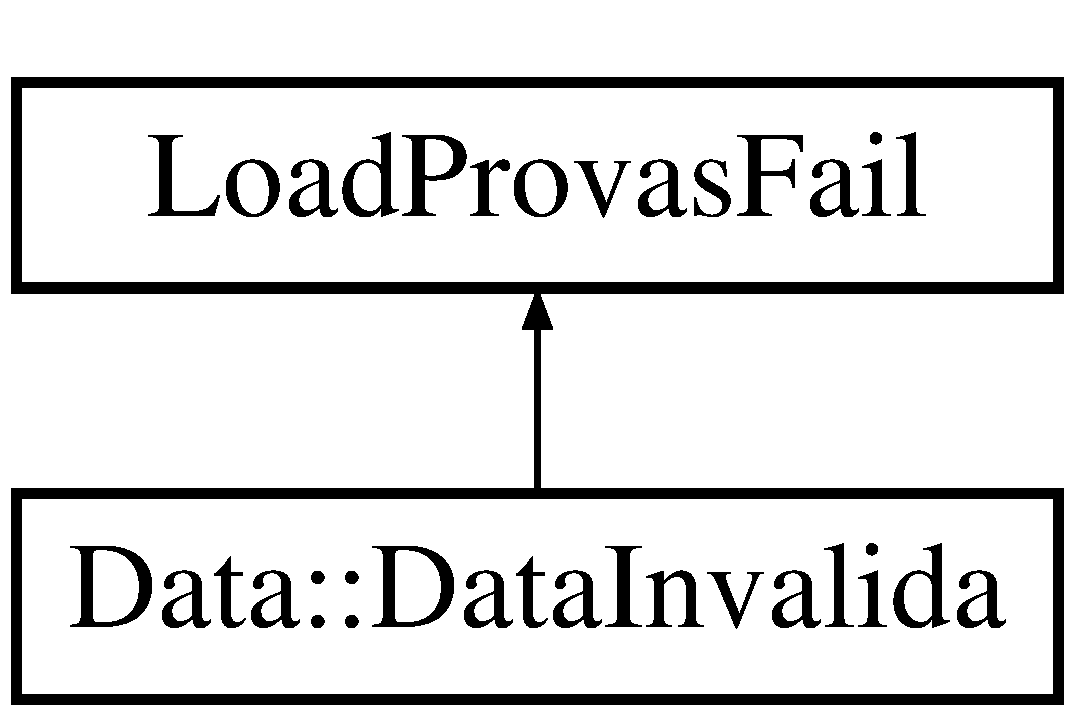
\includegraphics[height=2.000000cm]{class_data_1_1_data_invalida}
\end{center}
\end{figure}
\subsection*{Public Member Functions}
\begin{DoxyCompactItemize}
\item 
\hyperlink{class_data_1_1_data_invalida_afa06e582c3a7125852388d16f97ebc97}{Data\+Invalida} (int a, int m, int d)
\item 
string \hyperlink{class_data_1_1_data_invalida_abd5d99a7c864cc55b69424e4241aaf20}{get\+Message} () const 
\end{DoxyCompactItemize}


\subsection{Detailed Description}
\hyperlink{class_data_1_1_data_invalida}{Data\+Invalida}

Uma expecao de quando a data for invalida ou nao estiver dentro dos limites 

\subsection{Constructor \& Destructor Documentation}
\hypertarget{class_data_1_1_data_invalida_afa06e582c3a7125852388d16f97ebc97}{}\index{Data\+::\+Data\+Invalida@{Data\+::\+Data\+Invalida}!Data\+Invalida@{Data\+Invalida}}
\index{Data\+Invalida@{Data\+Invalida}!Data\+::\+Data\+Invalida@{Data\+::\+Data\+Invalida}}
\subsubsection[{Data\+Invalida(int a, int m, int d)}]{\setlength{\rightskip}{0pt plus 5cm}Data\+::\+Data\+Invalida\+::\+Data\+Invalida (
\begin{DoxyParamCaption}
\item[{int}]{a, }
\item[{int}]{m, }
\item[{int}]{d}
\end{DoxyParamCaption}
)\hspace{0.3cm}{\ttfamily [inline]}}\label{class_data_1_1_data_invalida_afa06e582c3a7125852388d16f97ebc97}

\begin{DoxyParams}{Parameters}
{\em a} & -\/ ano \\
\hline
{\em m} & -\/ mes \\
\hline
{\em d} & -\/ dia \\
\hline
\end{DoxyParams}


\subsection{Member Function Documentation}
\hypertarget{class_data_1_1_data_invalida_abd5d99a7c864cc55b69424e4241aaf20}{}\index{Data\+::\+Data\+Invalida@{Data\+::\+Data\+Invalida}!get\+Message@{get\+Message}}
\index{get\+Message@{get\+Message}!Data\+::\+Data\+Invalida@{Data\+::\+Data\+Invalida}}
\subsubsection[{get\+Message() const }]{\setlength{\rightskip}{0pt plus 5cm}string Data\+::\+Data\+Invalida\+::get\+Message (
\begin{DoxyParamCaption}
{}
\end{DoxyParamCaption}
) const\hspace{0.3cm}{\ttfamily [inline]}, {\ttfamily [virtual]}}\label{class_data_1_1_data_invalida_abd5d99a7c864cc55b69424e4241aaf20}
Constroi uma mensagem como a data

\begin{DoxyReturn}{Returns}
uma string como uma mensagem 
\end{DoxyReturn}


Implements \hyperlink{class_load_provas_fail}{Load\+Provas\+Fail}.



The documentation for this class was generated from the following file\+:\begin{DoxyCompactItemize}
\item 
src/Data.\+h\end{DoxyCompactItemize}

\hypertarget{class_desporto}{}\section{Desporto Class Reference}
\label{class_desporto}\index{Desporto@{Desporto}}
\subsection*{Classes}
\begin{DoxyCompactItemize}
\item 
class \hyperlink{class_desporto_1_1_desporto_inexistente}{Desporto\+Inexistente}
\item 
class \hyperlink{class_desporto_1_1_modalidade_existe}{Modalidade\+Existe}
\end{DoxyCompactItemize}
\subsection*{Public Member Functions}
\begin{DoxyCompactItemize}
\item 
\hyperlink{class_desporto_af6abc41a2b8a416e475afb9409226ef6}{Desporto} ()
\item 
\hyperlink{class_desporto_a8f285da75c79fbbc353535296cd5f492}{Desporto} (string n, string pont, bool cresc)
\item 
\hypertarget{class_desporto_ab8a8413f056aeaa6dbd55730a7b6cd85}{}string {\bfseries get\+Nome} () const \label{class_desporto_ab8a8413f056aeaa6dbd55730a7b6cd85}

\item 
\hypertarget{class_desporto_a689058796c1401692f7b9630e882516f}{}string {\bfseries get\+Pontuacao} () const \label{class_desporto_a689058796c1401692f7b9630e882516f}

\item 
\hypertarget{class_desporto_a0b93c7fb93a29b1e960bed04b0aa048e}{}vector$<$ \hyperlink{class_modalidade}{Modalidade} $\ast$ $>$ {\bfseries get\+Modalidades} () const \label{class_desporto_a0b93c7fb93a29b1e960bed04b0aa048e}

\item 
\hypertarget{class_desporto_abdc20318ca9a2d4a724572100eb2f271}{}bool {\bfseries is\+Crescente} () const \label{class_desporto_abdc20318ca9a2d4a724572100eb2f271}

\item 
void \hyperlink{class_desporto_a51a8862940614dfed584f05e17fb7b68}{apaga\+Modalidade} (int indice)
\item 
bool \hyperlink{class_desporto_a0656b98e63e1b54a7e3b03e20e9ca8b3}{operator==} (const \hyperlink{class_desporto}{Desporto} \&c) const 
\item 
void \hyperlink{class_desporto_ae172dd6af2bbb85308d8f38a7f77fe33}{menu} ()
\item 
void \hyperlink{class_desporto_aa0bacf802c53d5422d0b6b9882c9a843}{menu\+Modalidades} ()
\item 
void \hyperlink{class_desporto_ac4c0ce9d5e637917a137fa9949fe7f41}{adiciona\+Modalidade} ()
\item 
void \hyperlink{class_desporto_a070694d6e2512119538fd12a26699e1e}{adiciona\+Modalidade} (\hyperlink{class_modalidade}{Modalidade} $\ast$m)
\end{DoxyCompactItemize}
\subsection*{Friends}
\begin{DoxyCompactItemize}
\item 
ostream \& \hyperlink{class_desporto_a521ed305078741a8eff6537a37502f95}{operator$<$$<$} (ostream \&o, const \hyperlink{class_desporto}{Desporto} \&d)
\end{DoxyCompactItemize}


\subsection{Constructor \& Destructor Documentation}
\hypertarget{class_desporto_af6abc41a2b8a416e475afb9409226ef6}{}\index{Desporto@{Desporto}!Desporto@{Desporto}}
\index{Desporto@{Desporto}!Desporto@{Desporto}}
\subsubsection[{Desporto()}]{\setlength{\rightskip}{0pt plus 5cm}Desporto\+::\+Desporto (
\begin{DoxyParamCaption}
{}
\end{DoxyParamCaption}
)}\label{class_desporto_af6abc41a2b8a416e475afb9409226ef6}
Construtor default \hypertarget{class_desporto_a8f285da75c79fbbc353535296cd5f492}{}\index{Desporto@{Desporto}!Desporto@{Desporto}}
\index{Desporto@{Desporto}!Desporto@{Desporto}}
\subsubsection[{Desporto(string n, string pont, bool cresc)}]{\setlength{\rightskip}{0pt plus 5cm}Desporto\+::\+Desporto (
\begin{DoxyParamCaption}
\item[{string}]{n, }
\item[{string}]{pont, }
\item[{bool}]{cresc}
\end{DoxyParamCaption}
)}\label{class_desporto_a8f285da75c79fbbc353535296cd5f492}
Construtor de \hyperlink{class_desporto}{Desporto}

inicializa nome, pontuacao.\+nome, pontuacao.\+crescente


\begin{DoxyParams}{Parameters}
{\em n} & -\/ nome do desporto \\
\hline
{\em pont} & -\/ tipo de pontuacao do desporto \\
\hline
{\em cresc} & -\/ true se a pontuacao e crecente ( se o vencedor � quem tem mais pontos) \\
\hline
\end{DoxyParams}


\subsection{Member Function Documentation}
\hypertarget{class_desporto_ac4c0ce9d5e637917a137fa9949fe7f41}{}\index{Desporto@{Desporto}!adiciona\+Modalidade@{adiciona\+Modalidade}}
\index{adiciona\+Modalidade@{adiciona\+Modalidade}!Desporto@{Desporto}}
\subsubsection[{adiciona\+Modalidade()}]{\setlength{\rightskip}{0pt plus 5cm}void Desporto\+::adiciona\+Modalidade (
\begin{DoxyParamCaption}
{}
\end{DoxyParamCaption}
)}\label{class_desporto_ac4c0ce9d5e637917a137fa9949fe7f41}
Mostra na interface um menu para criar uma nova modalidade

O utilizador tem de introduzir os dados para a criacao de uma nova modalidade e se todos forem validos O ela e criada e adicionada ao vetor modalidades \hypertarget{class_desporto_a070694d6e2512119538fd12a26699e1e}{}\index{Desporto@{Desporto}!adiciona\+Modalidade@{adiciona\+Modalidade}}
\index{adiciona\+Modalidade@{adiciona\+Modalidade}!Desporto@{Desporto}}
\subsubsection[{adiciona\+Modalidade(\+Modalidade $\ast$m)}]{\setlength{\rightskip}{0pt plus 5cm}void Desporto\+::adiciona\+Modalidade (
\begin{DoxyParamCaption}
\item[{{\bf Modalidade} $\ast$}]{m}
\end{DoxyParamCaption}
)}\label{class_desporto_a070694d6e2512119538fd12a26699e1e}
Adiciona uma modalidade nova ao vetor modalidades (para testes)

Verifica se a modalidade ja existe e se nao existir adiciona-\/a ao vetor modalidades


\begin{DoxyParams}{Parameters}
{\em m} & -\/modalidade a adicionar \\
\hline
\end{DoxyParams}
\hypertarget{class_desporto_a51a8862940614dfed584f05e17fb7b68}{}\index{Desporto@{Desporto}!apaga\+Modalidade@{apaga\+Modalidade}}
\index{apaga\+Modalidade@{apaga\+Modalidade}!Desporto@{Desporto}}
\subsubsection[{apaga\+Modalidade(int indice)}]{\setlength{\rightskip}{0pt plus 5cm}void Desporto\+::apaga\+Modalidade (
\begin{DoxyParamCaption}
\item[{int}]{indice}
\end{DoxyParamCaption}
)}\label{class_desporto_a51a8862940614dfed584f05e17fb7b68}
Retira modalidade do vetor de modalidades do desporto

Procura a modalidade de indice indice e retira-\/a o vetor modalidades


\begin{DoxyParams}{Parameters}
{\em indice} & -\/ indice da modalidade em modalidades \\
\hline
\end{DoxyParams}
\hypertarget{class_desporto_ae172dd6af2bbb85308d8f38a7f77fe33}{}\index{Desporto@{Desporto}!menu@{menu}}
\index{menu@{menu}!Desporto@{Desporto}}
\subsubsection[{menu()}]{\setlength{\rightskip}{0pt plus 5cm}void Desporto\+::menu (
\begin{DoxyParamCaption}
{}
\end{DoxyParamCaption}
)}\label{class_desporto_ae172dd6af2bbb85308d8f38a7f77fe33}
Mostra na interface um menu para o utilizador escolher que atributos do desporto quer mudar

O utilizador pode escolher entre mudar as modalidades, o tipo ou a hierarquia da pontuacao e o nome do desporto \hypertarget{class_desporto_aa0bacf802c53d5422d0b6b9882c9a843}{}\index{Desporto@{Desporto}!menu\+Modalidades@{menu\+Modalidades}}
\index{menu\+Modalidades@{menu\+Modalidades}!Desporto@{Desporto}}
\subsubsection[{menu\+Modalidades()}]{\setlength{\rightskip}{0pt plus 5cm}void Desporto\+::menu\+Modalidades (
\begin{DoxyParamCaption}
{}
\end{DoxyParamCaption}
)}\label{class_desporto_aa0bacf802c53d5422d0b6b9882c9a843}
Mostra na interface um menu para o utilizador alterar as modalidades do campeonato

O utilizador pode escolher entre alterar as modalidades existentes (� chamada a funcao menu\+Modalidades) e criar uma nova modalidade (e chamado o adiciona\+Modalidade) \hypertarget{class_desporto_a0656b98e63e1b54a7e3b03e20e9ca8b3}{}\index{Desporto@{Desporto}!operator==@{operator==}}
\index{operator==@{operator==}!Desporto@{Desporto}}
\subsubsection[{operator==(const Desporto \&c) const }]{\setlength{\rightskip}{0pt plus 5cm}bool Desporto\+::operator== (
\begin{DoxyParamCaption}
\item[{const {\bf Desporto} \&}]{c}
\end{DoxyParamCaption}
) const}\label{class_desporto_a0656b98e63e1b54a7e3b03e20e9ca8b3}
Compara dois desportos

Verifica se os dois desportos tem o mesmo nome


\begin{DoxyParams}{Parameters}
{\em c} & -\/ desporto a comparar \\
\hline
\end{DoxyParams}
\begin{DoxyReturn}{Returns}
true se os dois desportos tiverem o mesmo nome 
\end{DoxyReturn}


\subsection{Friends And Related Function Documentation}
\hypertarget{class_desporto_a521ed305078741a8eff6537a37502f95}{}\index{Desporto@{Desporto}!operator$<$$<$@{operator$<$$<$}}
\index{operator$<$$<$@{operator$<$$<$}!Desporto@{Desporto}}
\subsubsection[{operator$<$$<$}]{\setlength{\rightskip}{0pt plus 5cm}ostream\& operator$<$$<$ (
\begin{DoxyParamCaption}
\item[{ostream \&}]{o, }
\item[{const {\bf Desporto} \&}]{d}
\end{DoxyParamCaption}
)\hspace{0.3cm}{\ttfamily [friend]}}\label{class_desporto_a521ed305078741a8eff6537a37502f95}
Devolve um ostream com o nome do desporto

Preenche o com o nome do desporto


\begin{DoxyParams}{Parameters}
{\em o} & -\/ ostream a alterar \\
\hline
{\em d} & -\/ desporto cujo nome vai para o \\
\hline
\end{DoxyParams}
\begin{DoxyReturn}{Returns}
o, com o nome do desporto 
\end{DoxyReturn}


The documentation for this class was generated from the following files\+:\begin{DoxyCompactItemize}
\item 
src/Desporto.\+h\item 
src/Desporto.\+cpp\end{DoxyCompactItemize}

\hypertarget{class_campeonato_1_1_desporto_existe}{}\section{Campeonato\+:\+:Desporto\+Existe Class Reference}
\label{class_campeonato_1_1_desporto_existe}\index{Campeonato\+::\+Desporto\+Existe@{Campeonato\+::\+Desporto\+Existe}}


{\ttfamily \#include $<$Campeonato.\+h$>$}

\subsection*{Public Member Functions}
\begin{DoxyCompactItemize}
\item 
\hyperlink{class_campeonato_1_1_desporto_existe_a9a99e1ac4d2b7d6f431d368e7f5544f9}{Desporto\+Existe} ()
\item 
\hyperlink{class_campeonato_1_1_desporto_existe_a63f16592678722c636761e5a1020050b}{Desporto\+Existe} (string n)
\item 
\hypertarget{class_campeonato_1_1_desporto_existe_a8f21f30090933088d92912247d41cf13}{}string {\bfseries get\+Nome} () const \label{class_campeonato_1_1_desporto_existe_a8f21f30090933088d92912247d41cf13}

\end{DoxyCompactItemize}


\subsection{Detailed Description}
Classe \hyperlink{class_campeonato_1_1_desporto_existe}{Desporto\+Existe}

Uma excecao para o caso de tentarmos adicionar um \hyperlink{class_desporto}{Desporto} que ja exista no vetor desportos 

\subsection{Constructor \& Destructor Documentation}
\hypertarget{class_campeonato_1_1_desporto_existe_a9a99e1ac4d2b7d6f431d368e7f5544f9}{}\index{Campeonato\+::\+Desporto\+Existe@{Campeonato\+::\+Desporto\+Existe}!Desporto\+Existe@{Desporto\+Existe}}
\index{Desporto\+Existe@{Desporto\+Existe}!Campeonato\+::\+Desporto\+Existe@{Campeonato\+::\+Desporto\+Existe}}
\subsubsection[{Desporto\+Existe()}]{\setlength{\rightskip}{0pt plus 5cm}Campeonato\+::\+Desporto\+Existe\+::\+Desporto\+Existe (
\begin{DoxyParamCaption}
{}
\end{DoxyParamCaption}
)\hspace{0.3cm}{\ttfamily [inline]}}\label{class_campeonato_1_1_desporto_existe_a9a99e1ac4d2b7d6f431d368e7f5544f9}
Construtor default \hypertarget{class_campeonato_1_1_desporto_existe_a63f16592678722c636761e5a1020050b}{}\index{Campeonato\+::\+Desporto\+Existe@{Campeonato\+::\+Desporto\+Existe}!Desporto\+Existe@{Desporto\+Existe}}
\index{Desporto\+Existe@{Desporto\+Existe}!Campeonato\+::\+Desporto\+Existe@{Campeonato\+::\+Desporto\+Existe}}
\subsubsection[{Desporto\+Existe(string n)}]{\setlength{\rightskip}{0pt plus 5cm}Campeonato\+::\+Desporto\+Existe\+::\+Desporto\+Existe (
\begin{DoxyParamCaption}
\item[{string}]{n}
\end{DoxyParamCaption}
)\hspace{0.3cm}{\ttfamily [inline]}}\label{class_campeonato_1_1_desporto_existe_a63f16592678722c636761e5a1020050b}
Construtor \hyperlink{class_campeonato_1_1_desporto_existe}{Desporto\+Existe} \begin{DoxyVerb}   @param n - nome do desporto que causou a excecao\end{DoxyVerb}
 

The documentation for this class was generated from the following file\+:\begin{DoxyCompactItemize}
\item 
src/Campeonato.\+h\end{DoxyCompactItemize}

\hypertarget{class_desporto_1_1_desporto_inexistente}{}\section{Desporto\+:\+:Desporto\+Inexistente Class Reference}
\label{class_desporto_1_1_desporto_inexistente}\index{Desporto\+::\+Desporto\+Inexistente@{Desporto\+::\+Desporto\+Inexistente}}


{\ttfamily \#include $<$Desporto.\+h$>$}

\subsection*{Public Member Functions}
\begin{DoxyCompactItemize}
\item 
\hyperlink{class_desporto_1_1_desporto_inexistente_af927c111ca1ff3f0501b6b5d21089c76}{Desporto\+Inexistente} ()
\item 
\hyperlink{class_desporto_1_1_desporto_inexistente_a3d0e3632fd1bacb8ad9063dccf8694f6}{Desporto\+Inexistente} (string n)
\item 
string \hyperlink{class_desporto_1_1_desporto_inexistente_a258748916d7450e58399a63207b6ebfa}{get\+Message} () const 
\end{DoxyCompactItemize}


\subsection{Detailed Description}
Classe \hyperlink{class_desporto_1_1_desporto_inexistente}{Desporto\+Inexistente} Uma excecao para o caso de acedermos a um desporto inexistente 

\subsection{Constructor \& Destructor Documentation}
\hypertarget{class_desporto_1_1_desporto_inexistente_af927c111ca1ff3f0501b6b5d21089c76}{}\index{Desporto\+::\+Desporto\+Inexistente@{Desporto\+::\+Desporto\+Inexistente}!Desporto\+Inexistente@{Desporto\+Inexistente}}
\index{Desporto\+Inexistente@{Desporto\+Inexistente}!Desporto\+::\+Desporto\+Inexistente@{Desporto\+::\+Desporto\+Inexistente}}
\subsubsection[{Desporto\+Inexistente()}]{\setlength{\rightskip}{0pt plus 5cm}Desporto\+::\+Desporto\+Inexistente\+::\+Desporto\+Inexistente (
\begin{DoxyParamCaption}
{}
\end{DoxyParamCaption}
)\hspace{0.3cm}{\ttfamily [inline]}}\label{class_desporto_1_1_desporto_inexistente_af927c111ca1ff3f0501b6b5d21089c76}
Contrutor default

Uma excecao para o caso de acedermos a um desporto inexistente \hypertarget{class_desporto_1_1_desporto_inexistente_a3d0e3632fd1bacb8ad9063dccf8694f6}{}\index{Desporto\+::\+Desporto\+Inexistente@{Desporto\+::\+Desporto\+Inexistente}!Desporto\+Inexistente@{Desporto\+Inexistente}}
\index{Desporto\+Inexistente@{Desporto\+Inexistente}!Desporto\+::\+Desporto\+Inexistente@{Desporto\+::\+Desporto\+Inexistente}}
\subsubsection[{Desporto\+Inexistente(string n)}]{\setlength{\rightskip}{0pt plus 5cm}Desporto\+::\+Desporto\+Inexistente\+::\+Desporto\+Inexistente (
\begin{DoxyParamCaption}
\item[{string}]{n}
\end{DoxyParamCaption}
)\hspace{0.3cm}{\ttfamily [inline]}}\label{class_desporto_1_1_desporto_inexistente_a3d0e3632fd1bacb8ad9063dccf8694f6}
Contrutor \hyperlink{class_desporto_1_1_desporto_inexistente}{Desporto\+Inexistente}


\begin{DoxyParams}{Parameters}
{\em n} & -\/ nome do desporto que causou a excecao \\
\hline
\end{DoxyParams}


\subsection{Member Function Documentation}
\hypertarget{class_desporto_1_1_desporto_inexistente_a258748916d7450e58399a63207b6ebfa}{}\index{Desporto\+::\+Desporto\+Inexistente@{Desporto\+::\+Desporto\+Inexistente}!get\+Message@{get\+Message}}
\index{get\+Message@{get\+Message}!Desporto\+::\+Desporto\+Inexistente@{Desporto\+::\+Desporto\+Inexistente}}
\subsubsection[{get\+Message() const }]{\setlength{\rightskip}{0pt plus 5cm}string Desporto\+::\+Desporto\+Inexistente\+::get\+Message (
\begin{DoxyParamCaption}
{}
\end{DoxyParamCaption}
) const\hspace{0.3cm}{\ttfamily [inline]}}\label{class_desporto_1_1_desporto_inexistente_a258748916d7450e58399a63207b6ebfa}
Para imprimir mensagem de erro

\begin{DoxyReturn}{Returns}
mensagem a imprimir 
\end{DoxyReturn}


The documentation for this class was generated from the following file\+:\begin{DoxyCompactItemize}
\item 
src/Desporto.\+h\end{DoxyCompactItemize}

\hypertarget{class_equipa}{}\section{Equipa Class Reference}
\label{class_equipa}\index{Equipa@{Equipa}}


{\ttfamily \#include $<$Equipa.\+h$>$}

\subsection*{Classes}
\begin{DoxyCompactItemize}
\item 
class \hyperlink{class_equipa_1_1_atleta_existe}{Atleta\+Existe}
\item 
class \hyperlink{class_equipa_1_1_equipa_inexistente}{Equipa\+Inexistente}
\end{DoxyCompactItemize}
\subsection*{Public Member Functions}
\begin{DoxyCompactItemize}
\item 
\hyperlink{class_equipa_aa318e7b925bfed173bb90d20c63d8a43}{Equipa} (string n)
\item 
string \hyperlink{class_equipa_a9d20d0c8daa94e7562c5ea173337a224}{get\+Nome} () const 
\item 
vector$<$ \hyperlink{class_atleta}{Atleta} $\ast$ $>$ \hyperlink{class_equipa_a24c4de83cc1171ce42f442ef7be8a7c4}{get\+Atletas} () const 
\item 
vector$<$ \hyperlink{class_desporto}{Desporto} $\ast$ $>$ \hyperlink{class_equipa_a6b6996a193cea733caafb99d0ddebbcc}{get\+Desportos} () const 
\item 
void \hyperlink{class_equipa_a0e9f300d552f0c4de6fc28d555141eb5}{set\+Nome} (string n)
\item 
void \hyperlink{class_equipa_a3269b5a8f6c3ebc9370c4cdf004c0b31}{set\+Atletas} (vector$<$ \hyperlink{class_atleta}{Atleta} $\ast$ $>$ a)
\item 
void \hyperlink{class_equipa_ae94bfeafedcf21a1d85db42a7f60b4ea}{set\+Desportos} (vector$<$ \hyperlink{class_desporto}{Desporto} $\ast$ $>$ d)
\item 
bool \hyperlink{class_equipa_a18b0bb0b40831afda4d8baa0730dc40f}{adiciona\+Atleta} (\hyperlink{class_atleta}{Atleta} $\ast$a)
\item 
void \hyperlink{class_equipa_a22daef4c32fcc25228a113a134911565}{adiciona\+Desporto} (\hyperlink{class_desporto}{Desporto} $\ast$d)
\item 
void \hyperlink{class_equipa_a0ff737879e2ece8397d01d1da745a788}{apaga\+Modalidade} (int i\+\_\+atleta, int i\+\_\+modalidade)
\item 
void \hyperlink{class_equipa_ac2252ae9144c32ad2dfb227b9dfb2c15}{apaga\+Atleta} (string nome)
\item 
bool \hyperlink{class_equipa_a754b42e94c0ca91ac2c2a3890e7f3191}{operator==} (const \hyperlink{class_equipa}{Equipa} \&c) const 
\item 
\hyperlink{class_equipa}{Equipa} \& \hyperlink{class_equipa_a372f3177a2f628ddaff2c40ed7d26bf8}{operator=} (const \hyperlink{class_equipa}{Equipa} \&a)
\item 
void \hyperlink{class_equipa_ac2ab600cc917f8709aeda9a71a0a9aa4}{adicionar\+Desporto} (vector$<$ \hyperlink{class_desporto}{Desporto} $\ast$ $>$ Desp\+List)
\item 
void \hyperlink{class_equipa_a90fac8b1f621a9a82b4b32eb3efcdaa4}{retirar\+Desporto} ()
\item 
void \hyperlink{class_equipa_a44df4366958af97be66020a0f8e18a94}{menu} (vector$<$ \hyperlink{class_desporto}{Desporto} $\ast$ $>$ Desp\+List)
\item 
void \hyperlink{class_equipa_a8f8b5838284e2154abe8608f53ee2681}{menu\+Atletas} ()
\item 
void \hyperlink{class_equipa_afead1fbf9a337c39bb771b37dad578d3}{adiciona\+Atleta} ()
\end{DoxyCompactItemize}
\subsection*{Friends}
\begin{DoxyCompactItemize}
\item 
ostream \& \hyperlink{class_equipa_a45a67c28f3613161c95e9cfd11c055df}{operator$<$$<$} (ostream \&o, const \hyperlink{class_equipa}{Equipa} \&d)
\end{DoxyCompactItemize}


\subsection{Detailed Description}
Class \hyperlink{class_equipa}{Equipa}

Representa um conjunto de atletas 

\subsection{Constructor \& Destructor Documentation}
\hypertarget{class_equipa_aa318e7b925bfed173bb90d20c63d8a43}{}\index{Equipa@{Equipa}!Equipa@{Equipa}}
\index{Equipa@{Equipa}!Equipa@{Equipa}}
\subsubsection[{Equipa(string n)}]{\setlength{\rightskip}{0pt plus 5cm}Equipa\+::\+Equipa (
\begin{DoxyParamCaption}
\item[{string}]{n}
\end{DoxyParamCaption}
)}\label{class_equipa_aa318e7b925bfed173bb90d20c63d8a43}
Inicializa o nome


\begin{DoxyParams}{Parameters}
{\em n} & -\/ nome da equipa \\
\hline
\end{DoxyParams}


\subsection{Member Function Documentation}
\hypertarget{class_equipa_a18b0bb0b40831afda4d8baa0730dc40f}{}\index{Equipa@{Equipa}!adiciona\+Atleta@{adiciona\+Atleta}}
\index{adiciona\+Atleta@{adiciona\+Atleta}!Equipa@{Equipa}}
\subsubsection[{adiciona\+Atleta(\+Atleta $\ast$a)}]{\setlength{\rightskip}{0pt plus 5cm}bool Equipa\+::adiciona\+Atleta (
\begin{DoxyParamCaption}
\item[{{\bf Atleta} $\ast$}]{a}
\end{DoxyParamCaption}
)}\label{class_equipa_a18b0bb0b40831afda4d8baa0730dc40f}
adiciona um novo atleta se este ainda nao estiver na equipa 
\begin{DoxyParams}{Parameters}
{\em a} & -\/ um atleta \\
\hline
\end{DoxyParams}
\begin{DoxyReturn}{Returns}
true se conseguir adicionar, false se nao 
\end{DoxyReturn}
\hypertarget{class_equipa_afead1fbf9a337c39bb771b37dad578d3}{}\index{Equipa@{Equipa}!adiciona\+Atleta@{adiciona\+Atleta}}
\index{adiciona\+Atleta@{adiciona\+Atleta}!Equipa@{Equipa}}
\subsubsection[{adiciona\+Atleta()}]{\setlength{\rightskip}{0pt plus 5cm}void Equipa\+::adiciona\+Atleta (
\begin{DoxyParamCaption}
{}
\end{DoxyParamCaption}
)}\label{class_equipa_afead1fbf9a337c39bb771b37dad578d3}
Pede ao utilizador a informacao necessaria para criar um atleta, e cria-\/o. \hypertarget{class_equipa_a22daef4c32fcc25228a113a134911565}{}\index{Equipa@{Equipa}!adiciona\+Desporto@{adiciona\+Desporto}}
\index{adiciona\+Desporto@{adiciona\+Desporto}!Equipa@{Equipa}}
\subsubsection[{adiciona\+Desporto(\+Desporto $\ast$d)}]{\setlength{\rightskip}{0pt plus 5cm}void Equipa\+::adiciona\+Desporto (
\begin{DoxyParamCaption}
\item[{{\bf Desporto} $\ast$}]{d}
\end{DoxyParamCaption}
)}\label{class_equipa_a22daef4c32fcc25228a113a134911565}
adiciona um novo desporto se este ainda nao estiver na equipa 
\begin{DoxyParams}{Parameters}
{\em d} & -\/ um desporto \\
\hline
\end{DoxyParams}
\hypertarget{class_equipa_ac2ab600cc917f8709aeda9a71a0a9aa4}{}\index{Equipa@{Equipa}!adicionar\+Desporto@{adicionar\+Desporto}}
\index{adicionar\+Desporto@{adicionar\+Desporto}!Equipa@{Equipa}}
\subsubsection[{adicionar\+Desporto(vector$<$ Desporto $\ast$ $>$ Desp\+List)}]{\setlength{\rightskip}{0pt plus 5cm}void Equipa\+::adicionar\+Desporto (
\begin{DoxyParamCaption}
\item[{vector$<$ {\bf Desporto} $\ast$ $>$}]{Desp\+List}
\end{DoxyParamCaption}
)}\label{class_equipa_ac2ab600cc917f8709aeda9a71a0a9aa4}
Abre uma lista de desportos a partir do vector Desp\+List, e permite selecionar um , o qual e adicionado.


\begin{DoxyParams}{Parameters}
{\em Desp\+List} & -\/ Lista de desportos \\
\hline
\end{DoxyParams}
\hypertarget{class_equipa_ac2252ae9144c32ad2dfb227b9dfb2c15}{}\index{Equipa@{Equipa}!apaga\+Atleta@{apaga\+Atleta}}
\index{apaga\+Atleta@{apaga\+Atleta}!Equipa@{Equipa}}
\subsubsection[{apaga\+Atleta(string nome)}]{\setlength{\rightskip}{0pt plus 5cm}void Equipa\+::apaga\+Atleta (
\begin{DoxyParamCaption}
\item[{string}]{nome}
\end{DoxyParamCaption}
)}\label{class_equipa_ac2252ae9144c32ad2dfb227b9dfb2c15}
apaga o atleta de nome nome 
\begin{DoxyParams}{Parameters}
{\em nome} & -\/ nome do atleta \\
\hline
\end{DoxyParams}
\hypertarget{class_equipa_a0ff737879e2ece8397d01d1da745a788}{}\index{Equipa@{Equipa}!apaga\+Modalidade@{apaga\+Modalidade}}
\index{apaga\+Modalidade@{apaga\+Modalidade}!Equipa@{Equipa}}
\subsubsection[{apaga\+Modalidade(int i\+\_\+atleta, int i\+\_\+modalidade)}]{\setlength{\rightskip}{0pt plus 5cm}void Equipa\+::apaga\+Modalidade (
\begin{DoxyParamCaption}
\item[{int}]{i\+\_\+atleta, }
\item[{int}]{i\+\_\+modalidade}
\end{DoxyParamCaption}
)}\label{class_equipa_a0ff737879e2ece8397d01d1da745a788}
apaga a modalidade de indice i\+\_\+modalidade de um atleta de indice i\+\_\+atleta 
\begin{DoxyParams}{Parameters}
{\em i\+\_\+atleta} & -\/ indice do atleta \\
\hline
{\em i\+\_\+modalidade} & -\/ indice da modalidade \\
\hline
\end{DoxyParams}
\hypertarget{class_equipa_a24c4de83cc1171ce42f442ef7be8a7c4}{}\index{Equipa@{Equipa}!get\+Atletas@{get\+Atletas}}
\index{get\+Atletas@{get\+Atletas}!Equipa@{Equipa}}
\subsubsection[{get\+Atletas() const }]{\setlength{\rightskip}{0pt plus 5cm}vector$<$ {\bf Atleta} $\ast$ $>$ Equipa\+::get\+Atletas (
\begin{DoxyParamCaption}
{}
\end{DoxyParamCaption}
) const}\label{class_equipa_a24c4de83cc1171ce42f442ef7be8a7c4}
\begin{DoxyReturn}{Returns}
atletas 
\end{DoxyReturn}
\hypertarget{class_equipa_a6b6996a193cea733caafb99d0ddebbcc}{}\index{Equipa@{Equipa}!get\+Desportos@{get\+Desportos}}
\index{get\+Desportos@{get\+Desportos}!Equipa@{Equipa}}
\subsubsection[{get\+Desportos() const }]{\setlength{\rightskip}{0pt plus 5cm}vector$<$ {\bf Desporto} $\ast$ $>$ Equipa\+::get\+Desportos (
\begin{DoxyParamCaption}
{}
\end{DoxyParamCaption}
) const}\label{class_equipa_a6b6996a193cea733caafb99d0ddebbcc}
\begin{DoxyReturn}{Returns}
desportos 
\end{DoxyReturn}
\hypertarget{class_equipa_a9d20d0c8daa94e7562c5ea173337a224}{}\index{Equipa@{Equipa}!get\+Nome@{get\+Nome}}
\index{get\+Nome@{get\+Nome}!Equipa@{Equipa}}
\subsubsection[{get\+Nome() const }]{\setlength{\rightskip}{0pt plus 5cm}string Equipa\+::get\+Nome (
\begin{DoxyParamCaption}
{}
\end{DoxyParamCaption}
) const}\label{class_equipa_a9d20d0c8daa94e7562c5ea173337a224}
\begin{DoxyReturn}{Returns}
nome 
\end{DoxyReturn}
\hypertarget{class_equipa_a44df4366958af97be66020a0f8e18a94}{}\index{Equipa@{Equipa}!menu@{menu}}
\index{menu@{menu}!Equipa@{Equipa}}
\subsubsection[{menu(vector$<$ Desporto $\ast$ $>$ Desp\+List)}]{\setlength{\rightskip}{0pt plus 5cm}void Equipa\+::menu (
\begin{DoxyParamCaption}
\item[{vector$<$ {\bf Desporto} $\ast$ $>$}]{Desp\+List}
\end{DoxyParamCaption}
)}\label{class_equipa_a44df4366958af97be66020a0f8e18a94}
Abre um menu com as seguintes opcoes\+: Alterar Nome, Alterar Atletas, Inscrever em \hyperlink{class_desporto}{Desporto} e Desinscrever de \hyperlink{class_desporto}{Desporto} \hypertarget{class_equipa_a8f8b5838284e2154abe8608f53ee2681}{}\index{Equipa@{Equipa}!menu\+Atletas@{menu\+Atletas}}
\index{menu\+Atletas@{menu\+Atletas}!Equipa@{Equipa}}
\subsubsection[{menu\+Atletas()}]{\setlength{\rightskip}{0pt plus 5cm}void Equipa\+::menu\+Atletas (
\begin{DoxyParamCaption}
{}
\end{DoxyParamCaption}
)}\label{class_equipa_a8f8b5838284e2154abe8608f53ee2681}
Abre uma lista de selecao com todos os atletas da equipa, e permite escolher um ou adicionar um novo \hypertarget{class_equipa_a372f3177a2f628ddaff2c40ed7d26bf8}{}\index{Equipa@{Equipa}!operator=@{operator=}}
\index{operator=@{operator=}!Equipa@{Equipa}}
\subsubsection[{operator=(const Equipa \&a)}]{\setlength{\rightskip}{0pt plus 5cm}{\bf Equipa} \& Equipa\+::operator= (
\begin{DoxyParamCaption}
\item[{const {\bf Equipa} \&}]{a}
\end{DoxyParamCaption}
)}\label{class_equipa_a372f3177a2f628ddaff2c40ed7d26bf8}

\begin{DoxyParams}{Parameters}
{\em a} & -\/ uma equipa \\
\hline
\end{DoxyParams}
\begin{DoxyReturn}{Returns}
uma equipa igual a \char`\"{}a\char`\"{} 
\end{DoxyReturn}
\hypertarget{class_equipa_a754b42e94c0ca91ac2c2a3890e7f3191}{}\index{Equipa@{Equipa}!operator==@{operator==}}
\index{operator==@{operator==}!Equipa@{Equipa}}
\subsubsection[{operator==(const Equipa \&c) const }]{\setlength{\rightskip}{0pt plus 5cm}bool Equipa\+::operator== (
\begin{DoxyParamCaption}
\item[{const {\bf Equipa} \&}]{c}
\end{DoxyParamCaption}
) const}\label{class_equipa_a754b42e94c0ca91ac2c2a3890e7f3191}

\begin{DoxyParams}{Parameters}
{\em c} & -\/ uma equipa \\
\hline
\end{DoxyParams}
\begin{DoxyReturn}{Returns}
true se o nome de c e desta equipa forem iguais, false caso contrario. 
\end{DoxyReturn}
\hypertarget{class_equipa_a90fac8b1f621a9a82b4b32eb3efcdaa4}{}\index{Equipa@{Equipa}!retirar\+Desporto@{retirar\+Desporto}}
\index{retirar\+Desporto@{retirar\+Desporto}!Equipa@{Equipa}}
\subsubsection[{retirar\+Desporto()}]{\setlength{\rightskip}{0pt plus 5cm}void Equipa\+::retirar\+Desporto (
\begin{DoxyParamCaption}
{}
\end{DoxyParamCaption}
)}\label{class_equipa_a90fac8b1f621a9a82b4b32eb3efcdaa4}
Abre a lista a partir do vector desportos, e permite selecionar um , o qual e retirado. \hypertarget{class_equipa_a3269b5a8f6c3ebc9370c4cdf004c0b31}{}\index{Equipa@{Equipa}!set\+Atletas@{set\+Atletas}}
\index{set\+Atletas@{set\+Atletas}!Equipa@{Equipa}}
\subsubsection[{set\+Atletas(vector$<$ Atleta $\ast$ $>$ a)}]{\setlength{\rightskip}{0pt plus 5cm}void Equipa\+::set\+Atletas (
\begin{DoxyParamCaption}
\item[{vector$<$ {\bf Atleta} $\ast$ $>$}]{a}
\end{DoxyParamCaption}
)}\label{class_equipa_a3269b5a8f6c3ebc9370c4cdf004c0b31}
Altera atletas para a;


\begin{DoxyParams}{Parameters}
{\em a} & -\/ lista de atletas \\
\hline
\end{DoxyParams}
\hypertarget{class_equipa_ae94bfeafedcf21a1d85db42a7f60b4ea}{}\index{Equipa@{Equipa}!set\+Desportos@{set\+Desportos}}
\index{set\+Desportos@{set\+Desportos}!Equipa@{Equipa}}
\subsubsection[{set\+Desportos(vector$<$ Desporto $\ast$ $>$ d)}]{\setlength{\rightskip}{0pt plus 5cm}void Equipa\+::set\+Desportos (
\begin{DoxyParamCaption}
\item[{vector$<$ {\bf Desporto} $\ast$ $>$}]{d}
\end{DoxyParamCaption}
)}\label{class_equipa_ae94bfeafedcf21a1d85db42a7f60b4ea}
Altera desportos para d;


\begin{DoxyParams}{Parameters}
{\em d} & -\/ lista de desportos \\
\hline
\end{DoxyParams}
\hypertarget{class_equipa_a0e9f300d552f0c4de6fc28d555141eb5}{}\index{Equipa@{Equipa}!set\+Nome@{set\+Nome}}
\index{set\+Nome@{set\+Nome}!Equipa@{Equipa}}
\subsubsection[{set\+Nome(string n)}]{\setlength{\rightskip}{0pt plus 5cm}void Equipa\+::set\+Nome (
\begin{DoxyParamCaption}
\item[{string}]{n}
\end{DoxyParamCaption}
)}\label{class_equipa_a0e9f300d552f0c4de6fc28d555141eb5}
Altera nome para n;


\begin{DoxyParams}{Parameters}
{\em n} & -\/ nome da equipa \\
\hline
\end{DoxyParams}


\subsection{Friends And Related Function Documentation}
\hypertarget{class_equipa_a45a67c28f3613161c95e9cfd11c055df}{}\index{Equipa@{Equipa}!operator$<$$<$@{operator$<$$<$}}
\index{operator$<$$<$@{operator$<$$<$}!Equipa@{Equipa}}
\subsubsection[{operator$<$$<$}]{\setlength{\rightskip}{0pt plus 5cm}ostream\& operator$<$$<$ (
\begin{DoxyParamCaption}
\item[{ostream \&}]{o, }
\item[{const {\bf Equipa} \&}]{d}
\end{DoxyParamCaption}
)\hspace{0.3cm}{\ttfamily [friend]}}\label{class_equipa_a45a67c28f3613161c95e9cfd11c055df}
imprime o nome da equipa


\begin{DoxyParams}{Parameters}
{\em o} & -\/ stream de output \\
\hline
{\em d} & -\/ uma equipa \\
\hline
\end{DoxyParams}
\begin{DoxyReturn}{Returns}
o 
\end{DoxyReturn}


The documentation for this class was generated from the following files\+:\begin{DoxyCompactItemize}
\item 
src/Equipa.\+h\item 
src/Equipa.\+cpp\end{DoxyCompactItemize}

\hypertarget{class_campeonato_1_1_equipa_existe}{}\section{Campeonato\+:\+:Equipa\+Existe Class Reference}
\label{class_campeonato_1_1_equipa_existe}\index{Campeonato\+::\+Equipa\+Existe@{Campeonato\+::\+Equipa\+Existe}}


{\ttfamily \#include $<$Campeonato.\+h$>$}

\subsection*{Public Member Functions}
\begin{DoxyCompactItemize}
\item 
\hyperlink{class_campeonato_1_1_equipa_existe_a66255ab300e77646a298dc96b7c07d4b}{Equipa\+Existe} ()
\item 
\hyperlink{class_campeonato_1_1_equipa_existe_aea10f4410d04ca0a3c0c880b435312fb}{Equipa\+Existe} (string n)
\item 
\hypertarget{class_campeonato_1_1_equipa_existe_a56ab960e7ab688c066b6b63de1e28acb}{}string {\bfseries get\+Nome} () const \label{class_campeonato_1_1_equipa_existe_a56ab960e7ab688c066b6b63de1e28acb}

\end{DoxyCompactItemize}


\subsection{Detailed Description}
Classe \hyperlink{class_campeonato_1_1_equipa_existe}{Equipa\+Existe} \begin{DoxyVerb}Uma excecao para o caso de tentarmos adicionar uma Equipa que ja exista no vetor equipas\end{DoxyVerb}
 

\subsection{Constructor \& Destructor Documentation}
\hypertarget{class_campeonato_1_1_equipa_existe_a66255ab300e77646a298dc96b7c07d4b}{}\index{Campeonato\+::\+Equipa\+Existe@{Campeonato\+::\+Equipa\+Existe}!Equipa\+Existe@{Equipa\+Existe}}
\index{Equipa\+Existe@{Equipa\+Existe}!Campeonato\+::\+Equipa\+Existe@{Campeonato\+::\+Equipa\+Existe}}
\subsubsection[{Equipa\+Existe()}]{\setlength{\rightskip}{0pt plus 5cm}Campeonato\+::\+Equipa\+Existe\+::\+Equipa\+Existe (
\begin{DoxyParamCaption}
{}
\end{DoxyParamCaption}
)\hspace{0.3cm}{\ttfamily [inline]}}\label{class_campeonato_1_1_equipa_existe_a66255ab300e77646a298dc96b7c07d4b}
Construtor default \hypertarget{class_campeonato_1_1_equipa_existe_aea10f4410d04ca0a3c0c880b435312fb}{}\index{Campeonato\+::\+Equipa\+Existe@{Campeonato\+::\+Equipa\+Existe}!Equipa\+Existe@{Equipa\+Existe}}
\index{Equipa\+Existe@{Equipa\+Existe}!Campeonato\+::\+Equipa\+Existe@{Campeonato\+::\+Equipa\+Existe}}
\subsubsection[{Equipa\+Existe(string n)}]{\setlength{\rightskip}{0pt plus 5cm}Campeonato\+::\+Equipa\+Existe\+::\+Equipa\+Existe (
\begin{DoxyParamCaption}
\item[{string}]{n}
\end{DoxyParamCaption}
)\hspace{0.3cm}{\ttfamily [inline]}}\label{class_campeonato_1_1_equipa_existe_aea10f4410d04ca0a3c0c880b435312fb}
Construtor \hyperlink{class_campeonato_1_1_equipa_existe}{Equipa\+Existe} \begin{DoxyVerb}           @param n - nome da equipa que causou a excecao\end{DoxyVerb}
 

The documentation for this class was generated from the following file\+:\begin{DoxyCompactItemize}
\item 
src/Campeonato.\+h\end{DoxyCompactItemize}

\hypertarget{class_equipa_1_1_equipa_inexistente}{}\section{Equipa\+:\+:Equipa\+Inexistente Class Reference}
\label{class_equipa_1_1_equipa_inexistente}\index{Equipa\+::\+Equipa\+Inexistente@{Equipa\+::\+Equipa\+Inexistente}}


{\ttfamily \#include $<$Equipa.\+h$>$}

\subsection*{Public Member Functions}
\begin{DoxyCompactItemize}
\item 
\hyperlink{class_equipa_1_1_equipa_inexistente_a2f7d6f2f65f6fb1ba619a0128630e841}{Equipa\+Inexistente} (string n)
\item 
string \hyperlink{class_equipa_1_1_equipa_inexistente_acbc2d7590e7e1e6ed616908934ed0361}{get\+Nome} () const 
\end{DoxyCompactItemize}


\subsection{Detailed Description}
Classe \hyperlink{class_equipa_1_1_atleta_existe}{Atleta\+Existe}

Uma excecao para o caso de o atleta em causa nao existir na equipa 

\subsection{Constructor \& Destructor Documentation}
\hypertarget{class_equipa_1_1_equipa_inexistente_a2f7d6f2f65f6fb1ba619a0128630e841}{}\index{Equipa\+::\+Equipa\+Inexistente@{Equipa\+::\+Equipa\+Inexistente}!Equipa\+Inexistente@{Equipa\+Inexistente}}
\index{Equipa\+Inexistente@{Equipa\+Inexistente}!Equipa\+::\+Equipa\+Inexistente@{Equipa\+::\+Equipa\+Inexistente}}
\subsubsection[{Equipa\+Inexistente(string n)}]{\setlength{\rightskip}{0pt plus 5cm}Equipa\+::\+Equipa\+Inexistente\+::\+Equipa\+Inexistente (
\begin{DoxyParamCaption}
\item[{string}]{n}
\end{DoxyParamCaption}
)\hspace{0.3cm}{\ttfamily [inline]}}\label{class_equipa_1_1_equipa_inexistente_a2f7d6f2f65f6fb1ba619a0128630e841}
Inicializa o nome 
\begin{DoxyParams}{Parameters}
{\em n} & -\/ nome do atleta \\
\hline
\end{DoxyParams}


\subsection{Member Function Documentation}
\hypertarget{class_equipa_1_1_equipa_inexistente_acbc2d7590e7e1e6ed616908934ed0361}{}\index{Equipa\+::\+Equipa\+Inexistente@{Equipa\+::\+Equipa\+Inexistente}!get\+Nome@{get\+Nome}}
\index{get\+Nome@{get\+Nome}!Equipa\+::\+Equipa\+Inexistente@{Equipa\+::\+Equipa\+Inexistente}}
\subsubsection[{get\+Nome() const }]{\setlength{\rightskip}{0pt plus 5cm}string Equipa\+::\+Equipa\+Inexistente\+::get\+Nome (
\begin{DoxyParamCaption}
{}
\end{DoxyParamCaption}
) const\hspace{0.3cm}{\ttfamily [inline]}}\label{class_equipa_1_1_equipa_inexistente_acbc2d7590e7e1e6ed616908934ed0361}
\begin{DoxyReturn}{Returns}
nome 
\end{DoxyReturn}


The documentation for this class was generated from the following file\+:\begin{DoxyCompactItemize}
\item 
src/Equipa.\+h\end{DoxyCompactItemize}

\hypertarget{class_ficheiro_inexistente}{}\section{Ficheiro\+Inexistente Class Reference}
\label{class_ficheiro_inexistente}\index{Ficheiro\+Inexistente@{Ficheiro\+Inexistente}}
\subsection*{Public Member Functions}
\begin{DoxyCompactItemize}
\item 
\hypertarget{class_ficheiro_inexistente_a39c3a505a18c2c9d2d641ea7ccd7ab80}{}{\bfseries Ficheiro\+Inexistente} (string n)\label{class_ficheiro_inexistente_a39c3a505a18c2c9d2d641ea7ccd7ab80}

\item 
\hypertarget{class_ficheiro_inexistente_a276cc949c9cea98e8cb41c6ef39b650d}{}string {\bfseries get\+Nome} ()\label{class_ficheiro_inexistente_a276cc949c9cea98e8cb41c6ef39b650d}

\end{DoxyCompactItemize}


The documentation for this class was generated from the following file\+:\begin{DoxyCompactItemize}
\item 
src/Lists.\+h\end{DoxyCompactItemize}

\hypertarget{class_hora}{}\section{Hora Class Reference}
\label{class_hora}\index{Hora@{Hora}}


{\ttfamily \#include $<$Data.\+h$>$}

\subsection*{Classes}
\begin{DoxyCompactItemize}
\item 
class \hyperlink{class_hora_1_1_hora_invalida}{Hora\+Invalida}
\end{DoxyCompactItemize}
\subsection*{Public Member Functions}
\begin{DoxyCompactItemize}
\item 
\hyperlink{class_hora_acba1e481b72cf9af44cc3418b2db5d84}{Hora} (int h, int m)
\item 
\hyperlink{class_hora}{Hora} \hyperlink{class_hora_a4d20f25d9881fcf81572d5c6c6797afa}{operator+} (const \hyperlink{class_hora}{Hora} \&h) const 
\item 
bool \hyperlink{class_hora_a6640c1cebbbc73495ec36f0f1480ac35}{operator$<$} (const \hyperlink{class_hora}{Hora} \&h) const 
\item 
bool \hyperlink{class_hora_a837b9feb94fc55d8cd60a888185ee496}{operator$>$} (const \hyperlink{class_hora}{Hora} \&h) const 
\item 
int \hyperlink{class_hora_aa7fa11ebe86089fbb43d90e7ed432cb6}{get\+Horas} () const 
\item 
int \hyperlink{class_hora_afd7735ef6f6222904a77f22a8bbb80fd}{get\+Minutos} () const 
\end{DoxyCompactItemize}
\subsection*{Friends}
\begin{DoxyCompactItemize}
\item 
ostream \& \hyperlink{class_hora_a51fe201f7a8d2f4069b045da603fc7a1}{operator$<$$<$} (ostream \&o, const \hyperlink{class_hora}{Hora} \&h)
\end{DoxyCompactItemize}


\subsection{Detailed Description}
\hyperlink{class_hora}{Hora}

Representa uma hora 

\subsection{Constructor \& Destructor Documentation}
\hypertarget{class_hora_acba1e481b72cf9af44cc3418b2db5d84}{}\index{Hora@{Hora}!Hora@{Hora}}
\index{Hora@{Hora}!Hora@{Hora}}
\subsubsection[{Hora(int h, int m)}]{\setlength{\rightskip}{0pt plus 5cm}Hora\+::\+Hora (
\begin{DoxyParamCaption}
\item[{int}]{h, }
\item[{int}]{m}
\end{DoxyParamCaption}
)}\label{class_hora_acba1e481b72cf9af44cc3418b2db5d84}

\begin{DoxyItemize}
\item Inicializa os atributos 
\begin{DoxyParams}{Parameters}
{\em h} & -\/ horas \\
\hline
{\em m} & -\/ minutos \\
\hline
\end{DoxyParams}

\end{DoxyItemize}

\subsection{Member Function Documentation}
\hypertarget{class_hora_aa7fa11ebe86089fbb43d90e7ed432cb6}{}\index{Hora@{Hora}!get\+Horas@{get\+Horas}}
\index{get\+Horas@{get\+Horas}!Hora@{Hora}}
\subsubsection[{get\+Horas() const }]{\setlength{\rightskip}{0pt plus 5cm}int Hora\+::get\+Horas (
\begin{DoxyParamCaption}
{}
\end{DoxyParamCaption}
) const}\label{class_hora_aa7fa11ebe86089fbb43d90e7ed432cb6}
\begin{DoxyReturn}{Returns}
horas 
\end{DoxyReturn}
\hypertarget{class_hora_afd7735ef6f6222904a77f22a8bbb80fd}{}\index{Hora@{Hora}!get\+Minutos@{get\+Minutos}}
\index{get\+Minutos@{get\+Minutos}!Hora@{Hora}}
\subsubsection[{get\+Minutos() const }]{\setlength{\rightskip}{0pt plus 5cm}int Hora\+::get\+Minutos (
\begin{DoxyParamCaption}
{}
\end{DoxyParamCaption}
) const}\label{class_hora_afd7735ef6f6222904a77f22a8bbb80fd}
\begin{DoxyReturn}{Returns}
minutos 
\end{DoxyReturn}
\hypertarget{class_hora_a4d20f25d9881fcf81572d5c6c6797afa}{}\index{Hora@{Hora}!operator+@{operator+}}
\index{operator+@{operator+}!Hora@{Hora}}
\subsubsection[{operator+(const Hora \&h) const }]{\setlength{\rightskip}{0pt plus 5cm}{\bf Hora} Hora\+::operator+ (
\begin{DoxyParamCaption}
\item[{const {\bf Hora} \&}]{h}
\end{DoxyParamCaption}
) const}\label{class_hora_a4d20f25d9881fcf81572d5c6c6797afa}

\begin{DoxyParams}{Parameters}
{\em h} & -\/ uma hora \\
\hline
\end{DoxyParams}
\begin{DoxyReturn}{Returns}
a soma das horas 
\end{DoxyReturn}
\hypertarget{class_hora_a6640c1cebbbc73495ec36f0f1480ac35}{}\index{Hora@{Hora}!operator$<$@{operator$<$}}
\index{operator$<$@{operator$<$}!Hora@{Hora}}
\subsubsection[{operator$<$(const Hora \&h) const }]{\setlength{\rightskip}{0pt plus 5cm}bool Hora\+::operator$<$ (
\begin{DoxyParamCaption}
\item[{const {\bf Hora} \&}]{h}
\end{DoxyParamCaption}
) const}\label{class_hora_a6640c1cebbbc73495ec36f0f1480ac35}

\begin{DoxyParams}{Parameters}
{\em h} & -\/ uma hora \\
\hline
\end{DoxyParams}
\begin{DoxyReturn}{Returns}
true se h for maior que esta hora, false se nao 
\end{DoxyReturn}
\hypertarget{class_hora_a837b9feb94fc55d8cd60a888185ee496}{}\index{Hora@{Hora}!operator$>$@{operator$>$}}
\index{operator$>$@{operator$>$}!Hora@{Hora}}
\subsubsection[{operator$>$(const Hora \&h) const }]{\setlength{\rightskip}{0pt plus 5cm}bool Hora\+::operator$>$ (
\begin{DoxyParamCaption}
\item[{const {\bf Hora} \&}]{h}
\end{DoxyParamCaption}
) const}\label{class_hora_a837b9feb94fc55d8cd60a888185ee496}

\begin{DoxyParams}{Parameters}
{\em h} & -\/ uma hora \\
\hline
\end{DoxyParams}
\begin{DoxyReturn}{Returns}
true se h for menor que esta hora, false se nao 
\end{DoxyReturn}


\subsection{Friends And Related Function Documentation}
\hypertarget{class_hora_a51fe201f7a8d2f4069b045da603fc7a1}{}\index{Hora@{Hora}!operator$<$$<$@{operator$<$$<$}}
\index{operator$<$$<$@{operator$<$$<$}!Hora@{Hora}}
\subsubsection[{operator$<$$<$}]{\setlength{\rightskip}{0pt plus 5cm}ostream\& operator$<$$<$ (
\begin{DoxyParamCaption}
\item[{ostream \&}]{o, }
\item[{const {\bf Hora} \&}]{h}
\end{DoxyParamCaption}
)\hspace{0.3cm}{\ttfamily [friend]}}\label{class_hora_a51fe201f7a8d2f4069b045da603fc7a1}
imprime a data no formato H\+H\+:M\+M


\begin{DoxyParams}{Parameters}
{\em o} & -\/ stream de output \\
\hline
{\em h} & -\/ uma hora \\
\hline
\end{DoxyParams}
\begin{DoxyReturn}{Returns}
o 
\end{DoxyReturn}


The documentation for this class was generated from the following files\+:\begin{DoxyCompactItemize}
\item 
src/Data.\+h\item 
src/Data.\+cpp\end{DoxyCompactItemize}

\hypertarget{class_hora_1_1_hora_invalida}{}\section{Hora\+:\+:Hora\+Invalida Class Reference}
\label{class_hora_1_1_hora_invalida}\index{Hora\+::\+Hora\+Invalida@{Hora\+::\+Hora\+Invalida}}


{\ttfamily \#include $<$Data.\+h$>$}

Inheritance diagram for Hora\+:\+:Hora\+Invalida\+:\begin{figure}[H]
\begin{center}
\leavevmode
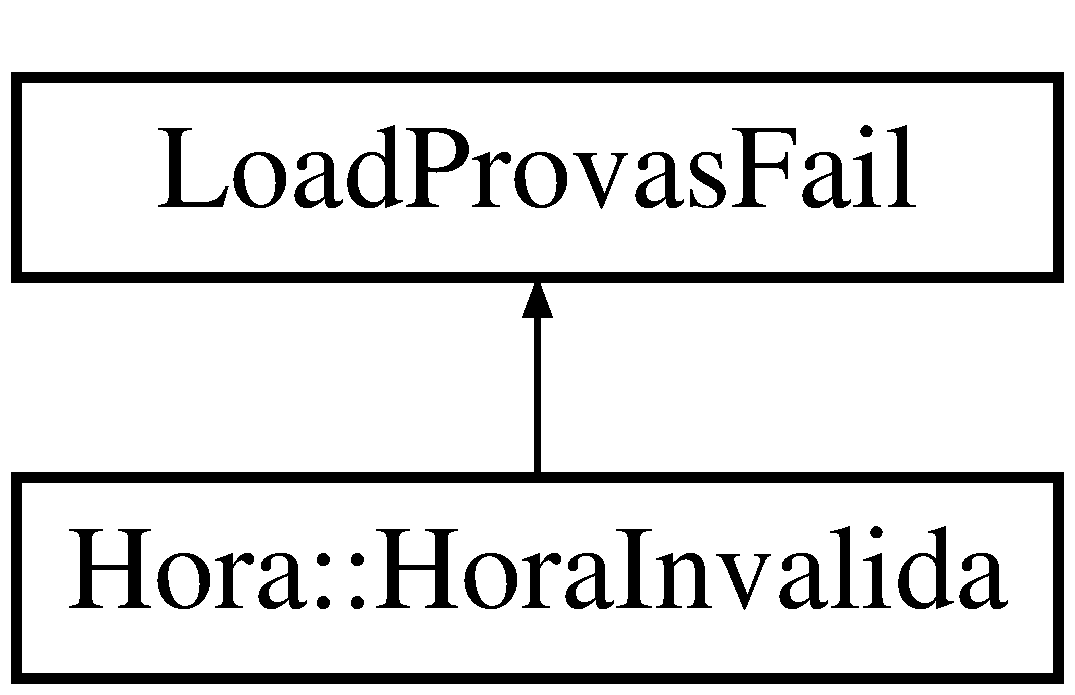
\includegraphics[height=2.000000cm]{class_hora_1_1_hora_invalida}
\end{center}
\end{figure}
\subsection*{Public Member Functions}
\begin{DoxyCompactItemize}
\item 
\hyperlink{class_hora_1_1_hora_invalida_a6d41a0a7cd476300a4f02c79b3d1651f}{Hora\+Invalida} (int h, int m)
\item 
string \hyperlink{class_hora_1_1_hora_invalida_ab214f94d7f1d40487b79584ff5b8b3cd}{get\+Message} () const 
\end{DoxyCompactItemize}


\subsection{Detailed Description}
Data\+Invalida

Uma expecao de quando a hora for invalida ou nao estiver dentro dos limites 

\subsection{Constructor \& Destructor Documentation}
\hypertarget{class_hora_1_1_hora_invalida_a6d41a0a7cd476300a4f02c79b3d1651f}{}\index{Hora\+::\+Hora\+Invalida@{Hora\+::\+Hora\+Invalida}!Hora\+Invalida@{Hora\+Invalida}}
\index{Hora\+Invalida@{Hora\+Invalida}!Hora\+::\+Hora\+Invalida@{Hora\+::\+Hora\+Invalida}}
\subsubsection[{Hora\+Invalida(int h, int m)}]{\setlength{\rightskip}{0pt plus 5cm}Hora\+::\+Hora\+Invalida\+::\+Hora\+Invalida (
\begin{DoxyParamCaption}
\item[{int}]{h, }
\item[{int}]{m}
\end{DoxyParamCaption}
)\hspace{0.3cm}{\ttfamily [inline]}}\label{class_hora_1_1_hora_invalida_a6d41a0a7cd476300a4f02c79b3d1651f}

\begin{DoxyItemize}
\item Inicializa os atributos 
\begin{DoxyParams}{Parameters}
{\em h} & -\/ horas \\
\hline
{\em m} & -\/ minutos \\
\hline
\end{DoxyParams}

\end{DoxyItemize}

\subsection{Member Function Documentation}
\hypertarget{class_hora_1_1_hora_invalida_ab214f94d7f1d40487b79584ff5b8b3cd}{}\index{Hora\+::\+Hora\+Invalida@{Hora\+::\+Hora\+Invalida}!get\+Message@{get\+Message}}
\index{get\+Message@{get\+Message}!Hora\+::\+Hora\+Invalida@{Hora\+::\+Hora\+Invalida}}
\subsubsection[{get\+Message() const }]{\setlength{\rightskip}{0pt plus 5cm}string Hora\+::\+Hora\+Invalida\+::get\+Message (
\begin{DoxyParamCaption}
{}
\end{DoxyParamCaption}
) const\hspace{0.3cm}{\ttfamily [inline]}, {\ttfamily [virtual]}}\label{class_hora_1_1_hora_invalida_ab214f94d7f1d40487b79584ff5b8b3cd}
Constroi uma mensagem como a hora

\begin{DoxyReturn}{Returns}
uma string como uma mensagem 
\end{DoxyReturn}


Implements \hyperlink{class_load_provas_fail}{Load\+Provas\+Fail}.



The documentation for this class was generated from the following file\+:\begin{DoxyCompactItemize}
\item 
src/Data.\+h\end{DoxyCompactItemize}

\hypertarget{class_campeonato_1_1_hora_invalida}{}\section{Campeonato\+:\+:Hora\+Invalida Class Reference}
\label{class_campeonato_1_1_hora_invalida}\index{Campeonato\+::\+Hora\+Invalida@{Campeonato\+::\+Hora\+Invalida}}


{\ttfamily \#include $<$Campeonato.\+h$>$}

\subsection*{Public Member Functions}
\begin{DoxyCompactItemize}
\item 
\hyperlink{class_campeonato_1_1_hora_invalida_a86c055a083548dcdd91200c129f4c455}{Hora\+Invalida} ()
\item 
\hyperlink{class_campeonato_1_1_hora_invalida_a8165c716bfae962843209e5cc9559f41}{Hora\+Invalida} (\hyperlink{class_hora}{Hora} h)
\item 
\hypertarget{class_campeonato_1_1_hora_invalida_ab47bee0b6238cdd0dc178b14a86374db}{}\hyperlink{class_hora}{Hora} {\bfseries get\+Hora} () const \label{class_campeonato_1_1_hora_invalida_ab47bee0b6238cdd0dc178b14a86374db}

\end{DoxyCompactItemize}


\subsection{Detailed Description}
Classe \hyperlink{class_campeonato_1_1_hora_invalida}{Hora\+Invalida} \begin{DoxyVerb}Uma excecao para o caso de tentarmos criar uma Hora fora dos limites do campeonato ou com horas/minutos invalidos\end{DoxyVerb}
 

\subsection{Constructor \& Destructor Documentation}
\hypertarget{class_campeonato_1_1_hora_invalida_a86c055a083548dcdd91200c129f4c455}{}\index{Campeonato\+::\+Hora\+Invalida@{Campeonato\+::\+Hora\+Invalida}!Hora\+Invalida@{Hora\+Invalida}}
\index{Hora\+Invalida@{Hora\+Invalida}!Campeonato\+::\+Hora\+Invalida@{Campeonato\+::\+Hora\+Invalida}}
\subsubsection[{Hora\+Invalida()}]{\setlength{\rightskip}{0pt plus 5cm}Campeonato\+::\+Hora\+Invalida\+::\+Hora\+Invalida (
\begin{DoxyParamCaption}
{}
\end{DoxyParamCaption}
)\hspace{0.3cm}{\ttfamily [inline]}}\label{class_campeonato_1_1_hora_invalida_a86c055a083548dcdd91200c129f4c455}
Construtor default \hypertarget{class_campeonato_1_1_hora_invalida_a8165c716bfae962843209e5cc9559f41}{}\index{Campeonato\+::\+Hora\+Invalida@{Campeonato\+::\+Hora\+Invalida}!Hora\+Invalida@{Hora\+Invalida}}
\index{Hora\+Invalida@{Hora\+Invalida}!Campeonato\+::\+Hora\+Invalida@{Campeonato\+::\+Hora\+Invalida}}
\subsubsection[{Hora\+Invalida(\+Hora h)}]{\setlength{\rightskip}{0pt plus 5cm}Campeonato\+::\+Hora\+Invalida\+::\+Hora\+Invalida (
\begin{DoxyParamCaption}
\item[{{\bf Hora}}]{h}
\end{DoxyParamCaption}
)\hspace{0.3cm}{\ttfamily [inline]}}\label{class_campeonato_1_1_hora_invalida_a8165c716bfae962843209e5cc9559f41}
Construtor \hyperlink{class_campeonato_1_1_hora_invalida}{Hora\+Invalida} \begin{DoxyVerb}               @param h - Hora que causou a excecao\end{DoxyVerb}
 

The documentation for this class was generated from the following file\+:\begin{DoxyCompactItemize}
\item 
src/Campeonato.\+h\end{DoxyCompactItemize}

\hypertarget{class_load_fail}{}\section{Load\+Fail Class Reference}
\label{class_load_fail}\index{Load\+Fail@{Load\+Fail}}
\subsection*{Public Member Functions}
\begin{DoxyCompactItemize}
\item 
\hypertarget{class_load_fail_a6f9c899a8e8007a40669fbe6613b332c}{}{\bfseries Load\+Fail} (string n)\label{class_load_fail_a6f9c899a8e8007a40669fbe6613b332c}

\item 
\hypertarget{class_load_fail_a75bcaf32324f43b3561acaaf5ba5dc43}{}string {\bfseries get\+Nome} ()\label{class_load_fail_a75bcaf32324f43b3561acaaf5ba5dc43}

\end{DoxyCompactItemize}


The documentation for this class was generated from the following file\+:\begin{DoxyCompactItemize}
\item 
src/Lists.\+h\end{DoxyCompactItemize}

\hypertarget{class_load_provas_fail}{}\section{Load\+Provas\+Fail Class Reference}
\label{class_load_provas_fail}\index{Load\+Provas\+Fail@{Load\+Provas\+Fail}}
Inheritance diagram for Load\+Provas\+Fail\+:\begin{figure}[H]
\begin{center}
\leavevmode
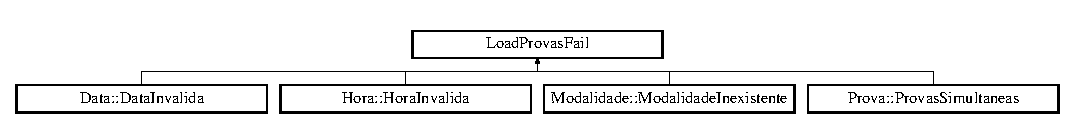
\includegraphics[height=1.290323cm]{class_load_provas_fail}
\end{center}
\end{figure}
\subsection*{Public Member Functions}
\begin{DoxyCompactItemize}
\item 
\hypertarget{class_load_provas_fail_a46bb569d3369817320b2037dc6d8a14f}{}virtual string {\bfseries get\+Message} () const  =0\label{class_load_provas_fail_a46bb569d3369817320b2037dc6d8a14f}

\end{DoxyCompactItemize}


The documentation for this class was generated from the following file\+:\begin{DoxyCompactItemize}
\item 
src/Lists.\+h\end{DoxyCompactItemize}

\hypertarget{class_modalidade}{}\section{Modalidade Class Reference}
\label{class_modalidade}\index{Modalidade@{Modalidade}}


{\ttfamily \#include $<$Modalidade.\+h$>$}

\subsection*{Classes}
\begin{DoxyCompactItemize}
\item 
class \hyperlink{class_modalidade_1_1_modalidade_inexistente}{Modalidade\+Inexistente}
\end{DoxyCompactItemize}
\subsection*{Public Member Functions}
\begin{DoxyCompactItemize}
\item 
\hyperlink{class_modalidade_ab70be2e5b2bf7a96a6e6a023f99b0c4b}{Modalidade} (string n, int h, int m, \hyperlink{class_desporto}{Desporto} $\ast$d)
\item 
string \hyperlink{class_modalidade_a46003f6a0dceac894f92971a6df9e4a7}{get\+Nome} () const 
\item 
\hyperlink{class_hora}{Hora} \hyperlink{class_modalidade_a7328b4411500160244ca64183478a5c1}{get\+Duracao} () const 
\item 
\hyperlink{class_desporto}{Desporto} $\ast$ \hyperlink{class_modalidade_ad128148792b93ca028b9cbcf73989bdd}{get\+Desporto} () const 
\item 
bool \hyperlink{class_modalidade_a502ce8cade8d9a04bc946ca5c3d6b0ca}{operator==} (const \hyperlink{class_modalidade}{Modalidade} \&c) const 
\item 
void \hyperlink{class_modalidade_a96cf31bec8dccd09e83b23d7d44925b3}{menu} ()
\end{DoxyCompactItemize}
\subsection*{Friends}
\begin{DoxyCompactItemize}
\item 
ostream \& \hyperlink{class_modalidade_a0068376dcbf60055a775ed885687e6e8}{operator$<$$<$} (ostream \&o, const \hyperlink{class_modalidade}{Modalidade} \&d)
\end{DoxyCompactItemize}


\subsection{Detailed Description}
Classe \hyperlink{class_modalidade}{Modalidade} Gere um tipo de prova, isto e uma modalidade.

\begin{DoxyAuthor}{Author}
Claudia Marinho, Daniela Sa, Joao Costa 
\end{DoxyAuthor}
\begin{DoxyDate}{Date}
08/11/2015 
\end{DoxyDate}


\subsection{Constructor \& Destructor Documentation}
\hypertarget{class_modalidade_ab70be2e5b2bf7a96a6e6a023f99b0c4b}{}\index{Modalidade@{Modalidade}!Modalidade@{Modalidade}}
\index{Modalidade@{Modalidade}!Modalidade@{Modalidade}}
\subsubsection[{Modalidade(string n, int h, int m, Desporto $\ast$d)}]{\setlength{\rightskip}{0pt plus 5cm}Modalidade\+::\+Modalidade (
\begin{DoxyParamCaption}
\item[{string}]{n, }
\item[{int}]{h, }
\item[{int}]{m, }
\item[{{\bf Desporto} $\ast$}]{d}
\end{DoxyParamCaption}
)}\label{class_modalidade_ab70be2e5b2bf7a96a6e6a023f99b0c4b}

\begin{DoxyParams}{Parameters}
{\em n} & -\/ nome da modalidade \\
\hline
{\em h} & -\/ numero de horas que dura uma prova da modalidade \\
\hline
{\em m} & -\/ numero de minutos que dura uma prova da modalidade \\
\hline
{\em d} & -\/ desporto ao qual pertence a modalidade \\
\hline
\end{DoxyParams}


\subsection{Member Function Documentation}
\hypertarget{class_modalidade_ad128148792b93ca028b9cbcf73989bdd}{}\index{Modalidade@{Modalidade}!get\+Desporto@{get\+Desporto}}
\index{get\+Desporto@{get\+Desporto}!Modalidade@{Modalidade}}
\subsubsection[{get\+Desporto() const }]{\setlength{\rightskip}{0pt plus 5cm}{\bf Desporto} $\ast$ Modalidade\+::get\+Desporto (
\begin{DoxyParamCaption}
{}
\end{DoxyParamCaption}
) const}\label{class_modalidade_ad128148792b93ca028b9cbcf73989bdd}
\begin{DoxyReturn}{Returns}
desporto 
\end{DoxyReturn}
\hypertarget{class_modalidade_a7328b4411500160244ca64183478a5c1}{}\index{Modalidade@{Modalidade}!get\+Duracao@{get\+Duracao}}
\index{get\+Duracao@{get\+Duracao}!Modalidade@{Modalidade}}
\subsubsection[{get\+Duracao() const }]{\setlength{\rightskip}{0pt plus 5cm}{\bf Hora} Modalidade\+::get\+Duracao (
\begin{DoxyParamCaption}
{}
\end{DoxyParamCaption}
) const}\label{class_modalidade_a7328b4411500160244ca64183478a5c1}
\begin{DoxyReturn}{Returns}
duracao 
\end{DoxyReturn}
\hypertarget{class_modalidade_a46003f6a0dceac894f92971a6df9e4a7}{}\index{Modalidade@{Modalidade}!get\+Nome@{get\+Nome}}
\index{get\+Nome@{get\+Nome}!Modalidade@{Modalidade}}
\subsubsection[{get\+Nome() const }]{\setlength{\rightskip}{0pt plus 5cm}string Modalidade\+::get\+Nome (
\begin{DoxyParamCaption}
{}
\end{DoxyParamCaption}
) const}\label{class_modalidade_a46003f6a0dceac894f92971a6df9e4a7}
\begin{DoxyReturn}{Returns}
nome 
\end{DoxyReturn}
\hypertarget{class_modalidade_a96cf31bec8dccd09e83b23d7d44925b3}{}\index{Modalidade@{Modalidade}!menu@{menu}}
\index{menu@{menu}!Modalidade@{Modalidade}}
\subsubsection[{menu()}]{\setlength{\rightskip}{0pt plus 5cm}void Modalidade\+::menu (
\begin{DoxyParamCaption}
{}
\end{DoxyParamCaption}
)}\label{class_modalidade_a96cf31bec8dccd09e83b23d7d44925b3}
Menu de Interface de uma modalidade

Mostra a seguinte opcao\+: (Alterar Nome) \hypertarget{class_modalidade_a502ce8cade8d9a04bc946ca5c3d6b0ca}{}\index{Modalidade@{Modalidade}!operator==@{operator==}}
\index{operator==@{operator==}!Modalidade@{Modalidade}}
\subsubsection[{operator==(const Modalidade \&c) const }]{\setlength{\rightskip}{0pt plus 5cm}bool Modalidade\+::operator== (
\begin{DoxyParamCaption}
\item[{const {\bf Modalidade} \&}]{c}
\end{DoxyParamCaption}
) const}\label{class_modalidade_a502ce8cade8d9a04bc946ca5c3d6b0ca}

\begin{DoxyParams}{Parameters}
{\em c} & -\/ uma modalidade \\
\hline
\end{DoxyParams}
\begin{DoxyReturn}{Returns}
true se o nome de c e desta modalidade forem iguais, false caso contrario. 
\end{DoxyReturn}


\subsection{Friends And Related Function Documentation}
\hypertarget{class_modalidade_a0068376dcbf60055a775ed885687e6e8}{}\index{Modalidade@{Modalidade}!operator$<$$<$@{operator$<$$<$}}
\index{operator$<$$<$@{operator$<$$<$}!Modalidade@{Modalidade}}
\subsubsection[{operator$<$$<$}]{\setlength{\rightskip}{0pt plus 5cm}ostream\& operator$<$$<$ (
\begin{DoxyParamCaption}
\item[{ostream \&}]{o, }
\item[{const {\bf Modalidade} \&}]{d}
\end{DoxyParamCaption}
)\hspace{0.3cm}{\ttfamily [friend]}}\label{class_modalidade_a0068376dcbf60055a775ed885687e6e8}
imprime o nome da modalidade


\begin{DoxyParams}{Parameters}
{\em o} & -\/ stream de output \\
\hline
{\em d} & -\/ uma modalidade \\
\hline
\end{DoxyParams}
\begin{DoxyReturn}{Returns}
o 
\end{DoxyReturn}


The documentation for this class was generated from the following files\+:\begin{DoxyCompactItemize}
\item 
src/Modalidade.\+h\item 
src/Modalidade.\+cpp\end{DoxyCompactItemize}

\hypertarget{class_desporto_1_1_modalidade_existe}{}\section{Desporto\+:\+:Modalidade\+Existe Class Reference}
\label{class_desporto_1_1_modalidade_existe}\index{Desporto\+::\+Modalidade\+Existe@{Desporto\+::\+Modalidade\+Existe}}


{\ttfamily \#include $<$Desporto.\+h$>$}

\subsection*{Public Member Functions}
\begin{DoxyCompactItemize}
\item 
\hyperlink{class_desporto_1_1_modalidade_existe_a5cae8a9dc1c166e0fbe75c0237066cc7}{Modalidade\+Existe} ()
\item 
\hyperlink{class_desporto_1_1_modalidade_existe_af3b0e08f186198e38bb6bb9f62281ee7}{Modalidade\+Existe} (string n)
\item 
string \hyperlink{class_desporto_1_1_modalidade_existe_aa0a6e98f34e7427a6606a5bb6b09ec48}{get\+Nome} () const 
\end{DoxyCompactItemize}


\subsection{Detailed Description}
Classe \hyperlink{class_desporto_1_1_modalidade_existe}{Modalidade\+Existe}

Uma excecao para o caso de tentarmos adicionar uma modalidade ja existente 

\subsection{Constructor \& Destructor Documentation}
\hypertarget{class_desporto_1_1_modalidade_existe_a5cae8a9dc1c166e0fbe75c0237066cc7}{}\index{Desporto\+::\+Modalidade\+Existe@{Desporto\+::\+Modalidade\+Existe}!Modalidade\+Existe@{Modalidade\+Existe}}
\index{Modalidade\+Existe@{Modalidade\+Existe}!Desporto\+::\+Modalidade\+Existe@{Desporto\+::\+Modalidade\+Existe}}
\subsubsection[{Modalidade\+Existe()}]{\setlength{\rightskip}{0pt plus 5cm}Desporto\+::\+Modalidade\+Existe\+::\+Modalidade\+Existe (
\begin{DoxyParamCaption}
{}
\end{DoxyParamCaption}
)\hspace{0.3cm}{\ttfamily [inline]}}\label{class_desporto_1_1_modalidade_existe_a5cae8a9dc1c166e0fbe75c0237066cc7}
Construtor default \hypertarget{class_desporto_1_1_modalidade_existe_af3b0e08f186198e38bb6bb9f62281ee7}{}\index{Desporto\+::\+Modalidade\+Existe@{Desporto\+::\+Modalidade\+Existe}!Modalidade\+Existe@{Modalidade\+Existe}}
\index{Modalidade\+Existe@{Modalidade\+Existe}!Desporto\+::\+Modalidade\+Existe@{Desporto\+::\+Modalidade\+Existe}}
\subsubsection[{Modalidade\+Existe(string n)}]{\setlength{\rightskip}{0pt plus 5cm}Desporto\+::\+Modalidade\+Existe\+::\+Modalidade\+Existe (
\begin{DoxyParamCaption}
\item[{string}]{n}
\end{DoxyParamCaption}
)\hspace{0.3cm}{\ttfamily [inline]}}\label{class_desporto_1_1_modalidade_existe_af3b0e08f186198e38bb6bb9f62281ee7}
Costrutor Modalidade\+Existente


\begin{DoxyParams}{Parameters}
{\em n} & -\/ nome da modalidade que causou a excecao \\
\hline
\end{DoxyParams}


\subsection{Member Function Documentation}
\hypertarget{class_desporto_1_1_modalidade_existe_aa0a6e98f34e7427a6606a5bb6b09ec48}{}\index{Desporto\+::\+Modalidade\+Existe@{Desporto\+::\+Modalidade\+Existe}!get\+Nome@{get\+Nome}}
\index{get\+Nome@{get\+Nome}!Desporto\+::\+Modalidade\+Existe@{Desporto\+::\+Modalidade\+Existe}}
\subsubsection[{get\+Nome() const }]{\setlength{\rightskip}{0pt plus 5cm}string Desporto\+::\+Modalidade\+Existe\+::get\+Nome (
\begin{DoxyParamCaption}
{}
\end{DoxyParamCaption}
) const\hspace{0.3cm}{\ttfamily [inline]}}\label{class_desporto_1_1_modalidade_existe_aa0a6e98f34e7427a6606a5bb6b09ec48}
Para imprimir mensagem de erro \begin{DoxyVerb}    @return mensagem a imprimir\end{DoxyVerb}
 

The documentation for this class was generated from the following file\+:\begin{DoxyCompactItemize}
\item 
src/Desporto.\+h\end{DoxyCompactItemize}

\hypertarget{class_modalidade_1_1_modalidade_inexistente}{}\section{Modalidade\+:\+:Modalidade\+Inexistente Class Reference}
\label{class_modalidade_1_1_modalidade_inexistente}\index{Modalidade\+::\+Modalidade\+Inexistente@{Modalidade\+::\+Modalidade\+Inexistente}}


{\ttfamily \#include $<$Modalidade.\+h$>$}

Inheritance diagram for Modalidade\+:\+:Modalidade\+Inexistente\+:\begin{figure}[H]
\begin{center}
\leavevmode
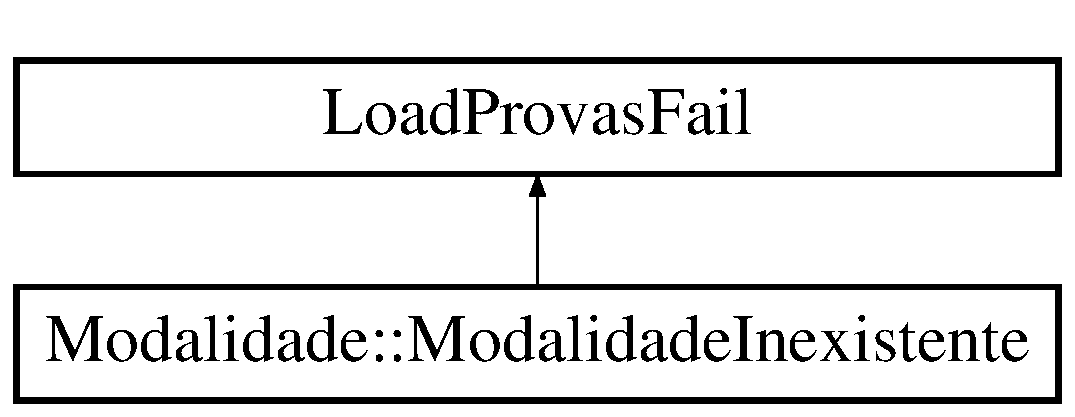
\includegraphics[height=2.000000cm]{class_modalidade_1_1_modalidade_inexistente}
\end{center}
\end{figure}
\subsection*{Public Member Functions}
\begin{DoxyCompactItemize}
\item 
\hyperlink{class_modalidade_1_1_modalidade_inexistente_abdc878e781526984595175bac47dd440}{Modalidade\+Inexistente} (string n)
\item 
string \hyperlink{class_modalidade_1_1_modalidade_inexistente_a79c5f308a9654ca8c08fdaac9fb6680f}{get\+Message} () const 
\end{DoxyCompactItemize}


\subsection{Detailed Description}
Classe \hyperlink{class_modalidade_1_1_modalidade_inexistente}{Modalidade\+Inexistente}

Uma expecao de nao existir uma modalidade em causa 

\subsection{Constructor \& Destructor Documentation}
\hypertarget{class_modalidade_1_1_modalidade_inexistente_abdc878e781526984595175bac47dd440}{}\index{Modalidade\+::\+Modalidade\+Inexistente@{Modalidade\+::\+Modalidade\+Inexistente}!Modalidade\+Inexistente@{Modalidade\+Inexistente}}
\index{Modalidade\+Inexistente@{Modalidade\+Inexistente}!Modalidade\+::\+Modalidade\+Inexistente@{Modalidade\+::\+Modalidade\+Inexistente}}
\subsubsection[{Modalidade\+Inexistente(string n)}]{\setlength{\rightskip}{0pt plus 5cm}Modalidade\+::\+Modalidade\+Inexistente\+::\+Modalidade\+Inexistente (
\begin{DoxyParamCaption}
\item[{string}]{n}
\end{DoxyParamCaption}
)\hspace{0.3cm}{\ttfamily [inline]}}\label{class_modalidade_1_1_modalidade_inexistente_abdc878e781526984595175bac47dd440}
Inicializa nome 
\begin{DoxyParams}{Parameters}
{\em n} & -\/ nome da modalidade \\
\hline
\end{DoxyParams}


\subsection{Member Function Documentation}
\hypertarget{class_modalidade_1_1_modalidade_inexistente_a79c5f308a9654ca8c08fdaac9fb6680f}{}\index{Modalidade\+::\+Modalidade\+Inexistente@{Modalidade\+::\+Modalidade\+Inexistente}!get\+Message@{get\+Message}}
\index{get\+Message@{get\+Message}!Modalidade\+::\+Modalidade\+Inexistente@{Modalidade\+::\+Modalidade\+Inexistente}}
\subsubsection[{get\+Message() const }]{\setlength{\rightskip}{0pt plus 5cm}string Modalidade\+::\+Modalidade\+Inexistente\+::get\+Message (
\begin{DoxyParamCaption}
{}
\end{DoxyParamCaption}
) const\hspace{0.3cm}{\ttfamily [inline]}, {\ttfamily [virtual]}}\label{class_modalidade_1_1_modalidade_inexistente_a79c5f308a9654ca8c08fdaac9fb6680f}
Constroi uma mensagem como o nome da modalidade

\begin{DoxyReturn}{Returns}
uma string como uma mensagem 
\end{DoxyReturn}


Implements \hyperlink{class_load_provas_fail}{Load\+Provas\+Fail}.



The documentation for this class was generated from the following file\+:\begin{DoxyCompactItemize}
\item 
src/Modalidade.\+h\end{DoxyCompactItemize}

\hypertarget{struct_pontuacao}{}\section{Pontuacao Struct Reference}
\label{struct_pontuacao}\index{Pontuacao@{Pontuacao}}
\subsection*{Public Attributes}
\begin{DoxyCompactItemize}
\item 
\hypertarget{struct_pontuacao_aa7d32400b2cc13f174fbd2c7a9c9d032}{}string {\bfseries nome}\label{struct_pontuacao_aa7d32400b2cc13f174fbd2c7a9c9d032}

\item 
\hypertarget{struct_pontuacao_a8b8590bcfcf51442e19e7384ecc8c446}{}bool {\bfseries crescente}\label{struct_pontuacao_a8b8590bcfcf51442e19e7384ecc8c446}

\end{DoxyCompactItemize}


The documentation for this struct was generated from the following file\+:\begin{DoxyCompactItemize}
\item 
src/Desporto.\+h\end{DoxyCompactItemize}

\hypertarget{class_prova}{}\section{Prova Class Reference}
\label{class_prova}\index{Prova@{Prova}}


{\ttfamily \#include $<$Prova.\+h$>$}

Inheritance diagram for Prova\+:\begin{figure}[H]
\begin{center}
\leavevmode
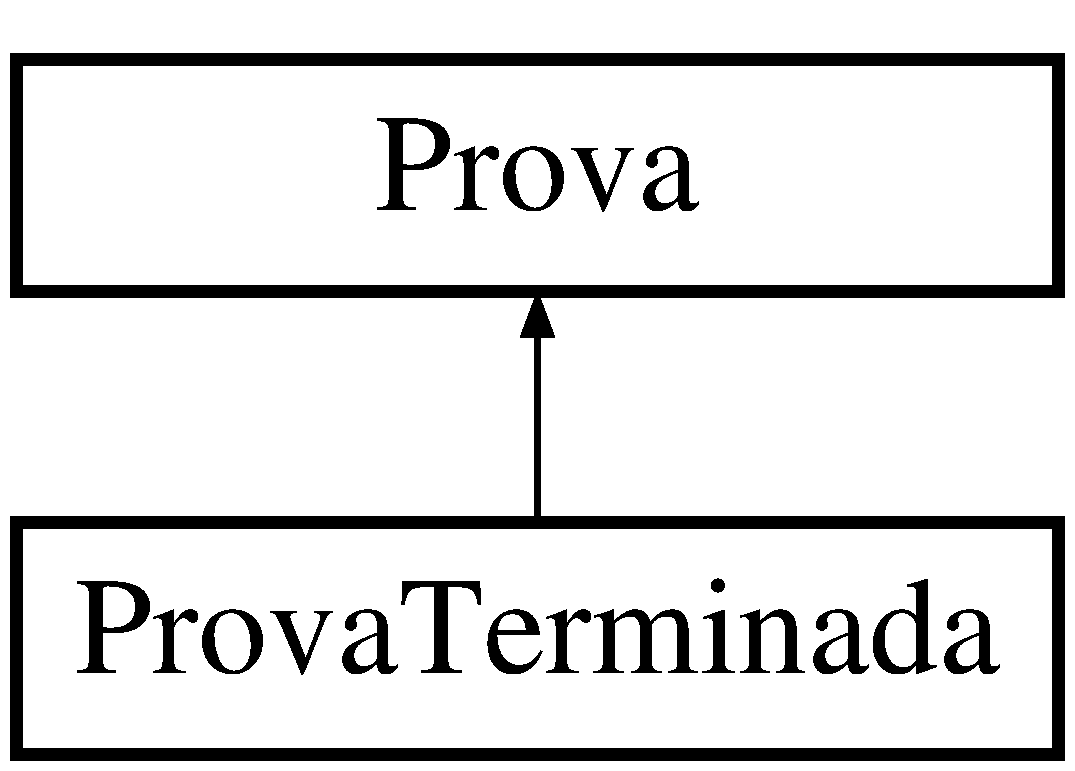
\includegraphics[height=2.000000cm]{class_prova}
\end{center}
\end{figure}
\subsection*{Classes}
\begin{DoxyCompactItemize}
\item 
class \hyperlink{class_prova_1_1_provas_simultaneas}{Provas\+Simultaneas}
\end{DoxyCompactItemize}
\subsection*{Public Member Functions}
\begin{DoxyCompactItemize}
\item 
\hyperlink{class_prova_a5d67d4424ea4ed03475ddcf80dee3539}{Prova} (\hyperlink{class_modalidade}{Modalidade} $\ast$m, \hyperlink{class_data}{Data} d, \hyperlink{class_hora}{Hora} i, char g)
\item 
\hyperlink{class_hora}{Hora} \hyperlink{class_prova_a27a6579ac4f103e53cbdd65d1f7994d1}{get\+Inicio} () const 
\item 
\hyperlink{class_hora}{Hora} \hyperlink{class_prova_aef874ac6cf95b34bd3b1574158cddc5f}{get\+Fim} () const 
\item 
\hyperlink{class_data}{Data} \hyperlink{class_prova_a2dbc83f56f67433d62246d9f69629b11}{get\+Data} () const 
\item 
\hyperlink{class_modalidade}{Modalidade} $\ast$ \hyperlink{class_prova_afbf918fbf8ddfd7a2b3785af51536e25}{get\+Modalidade} () const 
\item 
vector$<$ \hyperlink{class_atleta}{Atleta} $\ast$ $>$ \hyperlink{class_prova_a293abf27bb26c97f150be37c3a3e3636}{get\+Atletas} () const 
\item 
bool \hyperlink{class_prova_a5ebde6f5552c4459c0b5b7c677085a9e}{get\+Genero} () const 
\item 
bool \hyperlink{class_prova_abec8bb56f6e6e903b38aad4cc3f50e67}{get\+Realizada} () const 
\item 
void \hyperlink{class_prova_a6ef32c4d0f63b9576db83e4a8d63f390}{apaga\+Atleta} (string nome)
\item 
void \hyperlink{class_prova_abdb9448d1bc2efcb5b94265ddc73f4da}{adiciona\+Atleta} (\hyperlink{class_atleta}{Atleta} $\ast$a)
\item 
void \hyperlink{class_prova_a7c3eaa4b48561e50476739984f4c5648}{adicionar\+Atleta} (vector$<$ \hyperlink{class_equipa}{Equipa} $\ast$ $>$ Team\+List, vector$<$ \hyperlink{class_desporto}{Desporto} $\ast$ $>$ Desp\+List)
\item 
void \hyperlink{class_prova_aaee7c0aec1a890ab7e09e02f11f11d87}{retirar\+Atleta} ()
\item 
bool \hyperlink{class_prova_a0d9a660b9543ba8c8f9fb4509ff507d6}{Simultaneo} (\hyperlink{class_prova}{Prova} p)
\item 
void \hyperlink{class_prova_af8c2055a8a7e5edf94cacb5ef0d89e91}{menu} (vector$<$ \hyperlink{class_equipa}{Equipa} $\ast$ $>$ Team\+List, vector$<$ \hyperlink{class_desporto}{Desporto} $\ast$ $>$ Desp\+List)
\item 
bool \hyperlink{class_prova_a0da7d3508f91a710a250761498f7e9ba}{operator$<$} (const \hyperlink{class_prova}{Prova} \&p2) const 
\item 
bool \hyperlink{class_prova_a203f2d4d871609222a0621ae631bb1f5}{operator==} (const \hyperlink{class_prova}{Prova} \&p2) const 
\end{DoxyCompactItemize}
\subsection*{Protected Attributes}
\begin{DoxyCompactItemize}
\item 
\hypertarget{class_prova_a72061eddcdd4bbe05f083f812fd4c233}{}\hyperlink{class_modalidade}{Modalidade} $\ast$ {\bfseries modalidade}\label{class_prova_a72061eddcdd4bbe05f083f812fd4c233}

\item 
\hypertarget{class_prova_a18c9307475b75a77097e3f7b3b95359a}{}\hyperlink{class_data}{Data} {\bfseries data}\label{class_prova_a18c9307475b75a77097e3f7b3b95359a}

\item 
\hypertarget{class_prova_ae258a1a827472ff56e43910ff2b81a7e}{}\hyperlink{class_hora}{Hora} {\bfseries inicio}\label{class_prova_ae258a1a827472ff56e43910ff2b81a7e}

\item 
\hypertarget{class_prova_a67feb63b78712f2cd8aa0348c7e855ed}{}\hyperlink{class_hora}{Hora} {\bfseries fim}\label{class_prova_a67feb63b78712f2cd8aa0348c7e855ed}

\item 
\hypertarget{class_prova_a8561eecd9076cb8707eb99d90a89989d}{}vector$<$ \hyperlink{class_atleta}{Atleta} $\ast$ $>$ {\bfseries atletas}\label{class_prova_a8561eecd9076cb8707eb99d90a89989d}

\item 
\hypertarget{class_prova_a633da82d6916845b64bd5bdc2c6d6ad9}{}bool {\bfseries genero}\label{class_prova_a633da82d6916845b64bd5bdc2c6d6ad9}

\item 
\hypertarget{class_prova_ac2d537804224ac83c957db49ffcecef6}{}bool {\bfseries realizada}\label{class_prova_ac2d537804224ac83c957db49ffcecef6}

\end{DoxyCompactItemize}
\subsection*{Friends}
\begin{DoxyCompactItemize}
\item 
ostream \& \hyperlink{class_prova_a61b5beb563a366c43426f70b375cff61}{operator$<$$<$} (ostream \&o, const \hyperlink{class_prova}{Prova} \&p)
\end{DoxyCompactItemize}


\subsection{Detailed Description}
Class \hyperlink{class_prova}{Prova}

Representa um evento de uma modalidade 

\subsection{Constructor \& Destructor Documentation}
\hypertarget{class_prova_a5d67d4424ea4ed03475ddcf80dee3539}{}\index{Prova@{Prova}!Prova@{Prova}}
\index{Prova@{Prova}!Prova@{Prova}}
\subsubsection[{Prova(\+Modalidade $\ast$m, Data d, Hora i, char g)}]{\setlength{\rightskip}{0pt plus 5cm}Prova\+::\+Prova (
\begin{DoxyParamCaption}
\item[{{\bf Modalidade} $\ast$}]{m, }
\item[{{\bf Data}}]{d, }
\item[{{\bf Hora}}]{i, }
\item[{char}]{g}
\end{DoxyParamCaption}
)}\label{class_prova_a5d67d4424ea4ed03475ddcf80dee3539}

\begin{DoxyParams}{Parameters}
{\em m} & -\/ modalidade \\
\hline
{\em d} & -\/ data \\
\hline
{\em i} & -\/ hora \\
\hline
{\em g} & -\/ genero \\
\hline
\end{DoxyParams}


\subsection{Member Function Documentation}
\hypertarget{class_prova_abdb9448d1bc2efcb5b94265ddc73f4da}{}\index{Prova@{Prova}!adiciona\+Atleta@{adiciona\+Atleta}}
\index{adiciona\+Atleta@{adiciona\+Atleta}!Prova@{Prova}}
\subsubsection[{adiciona\+Atleta(\+Atleta $\ast$a)}]{\setlength{\rightskip}{0pt plus 5cm}void Prova\+::adiciona\+Atleta (
\begin{DoxyParamCaption}
\item[{{\bf Atleta} $\ast$}]{a}
\end{DoxyParamCaption}
)}\label{class_prova_abdb9448d1bc2efcb5b94265ddc73f4da}
Adiciona atleta ao vetor atletas 
\begin{DoxyParams}{Parameters}
{\em a} & -\/ atleta \\
\hline
\end{DoxyParams}
\hypertarget{class_prova_a7c3eaa4b48561e50476739984f4c5648}{}\index{Prova@{Prova}!adicionar\+Atleta@{adicionar\+Atleta}}
\index{adicionar\+Atleta@{adicionar\+Atleta}!Prova@{Prova}}
\subsubsection[{adicionar\+Atleta(vector$<$ Equipa $\ast$ $>$ Team\+List, vector$<$ Desporto $\ast$ $>$ Desp\+List)}]{\setlength{\rightskip}{0pt plus 5cm}void Prova\+::adicionar\+Atleta (
\begin{DoxyParamCaption}
\item[{vector$<$ {\bf Equipa} $\ast$ $>$}]{Team\+List, }
\item[{vector$<$ {\bf Desporto} $\ast$ $>$}]{Desp\+List}
\end{DoxyParamCaption}
)}\label{class_prova_a7c3eaa4b48561e50476739984f4c5648}
Permite ao utilizador escolher um atleta 
\begin{DoxyParams}{Parameters}
{\em Team\+List} & -\/ Lista de equipas \\
\hline
{\em Desp\+List} & -\/ Lista de desportos \\
\hline
\end{DoxyParams}
\hypertarget{class_prova_a6ef32c4d0f63b9576db83e4a8d63f390}{}\index{Prova@{Prova}!apaga\+Atleta@{apaga\+Atleta}}
\index{apaga\+Atleta@{apaga\+Atleta}!Prova@{Prova}}
\subsubsection[{apaga\+Atleta(string nome)}]{\setlength{\rightskip}{0pt plus 5cm}void Prova\+::apaga\+Atleta (
\begin{DoxyParamCaption}
\item[{string}]{nome}
\end{DoxyParamCaption}
)}\label{class_prova_a6ef32c4d0f63b9576db83e4a8d63f390}
Apaga o atleta de nome nome do vetor atletas 
\begin{DoxyParams}{Parameters}
{\em nome} & -\/ nome do atleta \\
\hline
\end{DoxyParams}
\hypertarget{class_prova_a293abf27bb26c97f150be37c3a3e3636}{}\index{Prova@{Prova}!get\+Atletas@{get\+Atletas}}
\index{get\+Atletas@{get\+Atletas}!Prova@{Prova}}
\subsubsection[{get\+Atletas() const }]{\setlength{\rightskip}{0pt plus 5cm}vector$<$ {\bf Atleta} $\ast$ $>$ Prova\+::get\+Atletas (
\begin{DoxyParamCaption}
{}
\end{DoxyParamCaption}
) const}\label{class_prova_a293abf27bb26c97f150be37c3a3e3636}
\begin{DoxyReturn}{Returns}
atletas 
\end{DoxyReturn}
\hypertarget{class_prova_a2dbc83f56f67433d62246d9f69629b11}{}\index{Prova@{Prova}!get\+Data@{get\+Data}}
\index{get\+Data@{get\+Data}!Prova@{Prova}}
\subsubsection[{get\+Data() const }]{\setlength{\rightskip}{0pt plus 5cm}{\bf Data} Prova\+::get\+Data (
\begin{DoxyParamCaption}
{}
\end{DoxyParamCaption}
) const}\label{class_prova_a2dbc83f56f67433d62246d9f69629b11}
\begin{DoxyReturn}{Returns}
data 
\end{DoxyReturn}
\hypertarget{class_prova_aef874ac6cf95b34bd3b1574158cddc5f}{}\index{Prova@{Prova}!get\+Fim@{get\+Fim}}
\index{get\+Fim@{get\+Fim}!Prova@{Prova}}
\subsubsection[{get\+Fim() const }]{\setlength{\rightskip}{0pt plus 5cm}{\bf Hora} Prova\+::get\+Fim (
\begin{DoxyParamCaption}
{}
\end{DoxyParamCaption}
) const}\label{class_prova_aef874ac6cf95b34bd3b1574158cddc5f}
\begin{DoxyReturn}{Returns}
fim 
\end{DoxyReturn}
\hypertarget{class_prova_a5ebde6f5552c4459c0b5b7c677085a9e}{}\index{Prova@{Prova}!get\+Genero@{get\+Genero}}
\index{get\+Genero@{get\+Genero}!Prova@{Prova}}
\subsubsection[{get\+Genero() const }]{\setlength{\rightskip}{0pt plus 5cm}bool Prova\+::get\+Genero (
\begin{DoxyParamCaption}
{}
\end{DoxyParamCaption}
) const}\label{class_prova_a5ebde6f5552c4459c0b5b7c677085a9e}
\begin{DoxyReturn}{Returns}
genero 
\end{DoxyReturn}
\hypertarget{class_prova_a27a6579ac4f103e53cbdd65d1f7994d1}{}\index{Prova@{Prova}!get\+Inicio@{get\+Inicio}}
\index{get\+Inicio@{get\+Inicio}!Prova@{Prova}}
\subsubsection[{get\+Inicio() const }]{\setlength{\rightskip}{0pt plus 5cm}{\bf Hora} Prova\+::get\+Inicio (
\begin{DoxyParamCaption}
{}
\end{DoxyParamCaption}
) const}\label{class_prova_a27a6579ac4f103e53cbdd65d1f7994d1}
\begin{DoxyReturn}{Returns}
inicio 
\end{DoxyReturn}
\hypertarget{class_prova_afbf918fbf8ddfd7a2b3785af51536e25}{}\index{Prova@{Prova}!get\+Modalidade@{get\+Modalidade}}
\index{get\+Modalidade@{get\+Modalidade}!Prova@{Prova}}
\subsubsection[{get\+Modalidade() const }]{\setlength{\rightskip}{0pt plus 5cm}{\bf Modalidade} $\ast$ Prova\+::get\+Modalidade (
\begin{DoxyParamCaption}
{}
\end{DoxyParamCaption}
) const}\label{class_prova_afbf918fbf8ddfd7a2b3785af51536e25}
\begin{DoxyReturn}{Returns}
modalidades 
\end{DoxyReturn}
\hypertarget{class_prova_abec8bb56f6e6e903b38aad4cc3f50e67}{}\index{Prova@{Prova}!get\+Realizada@{get\+Realizada}}
\index{get\+Realizada@{get\+Realizada}!Prova@{Prova}}
\subsubsection[{get\+Realizada() const }]{\setlength{\rightskip}{0pt plus 5cm}bool Prova\+::get\+Realizada (
\begin{DoxyParamCaption}
{}
\end{DoxyParamCaption}
) const}\label{class_prova_abec8bb56f6e6e903b38aad4cc3f50e67}
\begin{DoxyReturn}{Returns}
realizada 
\end{DoxyReturn}
\hypertarget{class_prova_af8c2055a8a7e5edf94cacb5ef0d89e91}{}\index{Prova@{Prova}!menu@{menu}}
\index{menu@{menu}!Prova@{Prova}}
\subsubsection[{menu(vector$<$ Equipa $\ast$ $>$ Team\+List, vector$<$ Desporto $\ast$ $>$ Desp\+List)}]{\setlength{\rightskip}{0pt plus 5cm}void Prova\+::menu (
\begin{DoxyParamCaption}
\item[{vector$<$ {\bf Equipa} $\ast$ $>$}]{Team\+List, }
\item[{vector$<$ {\bf Desporto} $\ast$ $>$}]{Desp\+List}
\end{DoxyParamCaption}
)}\label{class_prova_af8c2055a8a7e5edf94cacb5ef0d89e91}
Mostra as seguintes opcoes\+: (Alterar Atletas e Retirar Atletas) 
\begin{DoxyParams}{Parameters}
{\em Team\+List} & -\/ Lista de equipas \\
\hline
{\em Desp\+List} & -\/ Lista de desportos \\
\hline
\end{DoxyParams}
\hypertarget{class_prova_a0da7d3508f91a710a250761498f7e9ba}{}\index{Prova@{Prova}!operator$<$@{operator$<$}}
\index{operator$<$@{operator$<$}!Prova@{Prova}}
\subsubsection[{operator$<$(const Prova \&p2) const }]{\setlength{\rightskip}{0pt plus 5cm}bool Prova\+::operator$<$ (
\begin{DoxyParamCaption}
\item[{const {\bf Prova} \&}]{p2}
\end{DoxyParamCaption}
) const}\label{class_prova_a0da7d3508f91a710a250761498f7e9ba}

\begin{DoxyParams}{Parameters}
{\em p2} & -\/ prova \\
\hline
\end{DoxyParams}
\begin{DoxyReturn}{Returns}
true se occorer antes p2, false se nao 
\end{DoxyReturn}
\hypertarget{class_prova_a203f2d4d871609222a0621ae631bb1f5}{}\index{Prova@{Prova}!operator==@{operator==}}
\index{operator==@{operator==}!Prova@{Prova}}
\subsubsection[{operator==(const Prova \&p2) const }]{\setlength{\rightskip}{0pt plus 5cm}bool Prova\+::operator== (
\begin{DoxyParamCaption}
\item[{const {\bf Prova} \&}]{p2}
\end{DoxyParamCaption}
) const}\label{class_prova_a203f2d4d871609222a0621ae631bb1f5}

\begin{DoxyParams}{Parameters}
{\em p2} & -\/ prova \\
\hline
\end{DoxyParams}
\begin{DoxyReturn}{Returns}
true se forem iguais, false se nao 
\end{DoxyReturn}
\hypertarget{class_prova_aaee7c0aec1a890ab7e09e02f11f11d87}{}\index{Prova@{Prova}!retirar\+Atleta@{retirar\+Atleta}}
\index{retirar\+Atleta@{retirar\+Atleta}!Prova@{Prova}}
\subsubsection[{retirar\+Atleta()}]{\setlength{\rightskip}{0pt plus 5cm}void Prova\+::retirar\+Atleta (
\begin{DoxyParamCaption}
{}
\end{DoxyParamCaption}
)}\label{class_prova_aaee7c0aec1a890ab7e09e02f11f11d87}
Permite ao utilizador escolher um atleta para apagar \hypertarget{class_prova_a0d9a660b9543ba8c8f9fb4509ff507d6}{}\index{Prova@{Prova}!Simultaneo@{Simultaneo}}
\index{Simultaneo@{Simultaneo}!Prova@{Prova}}
\subsubsection[{Simultaneo(\+Prova p)}]{\setlength{\rightskip}{0pt plus 5cm}bool Prova\+::\+Simultaneo (
\begin{DoxyParamCaption}
\item[{{\bf Prova}}]{p}
\end{DoxyParamCaption}
)}\label{class_prova_a0d9a660b9543ba8c8f9fb4509ff507d6}

\begin{DoxyParams}{Parameters}
{\em p} & -\/ prova \\
\hline
\end{DoxyParams}
\begin{DoxyReturn}{Returns}
true se p e esta prova pertencerem ao mesmo desporto e forem em simultaneo 
\end{DoxyReturn}


\subsection{Friends And Related Function Documentation}
\hypertarget{class_prova_a61b5beb563a366c43426f70b375cff61}{}\index{Prova@{Prova}!operator$<$$<$@{operator$<$$<$}}
\index{operator$<$$<$@{operator$<$$<$}!Prova@{Prova}}
\subsubsection[{operator$<$$<$}]{\setlength{\rightskip}{0pt plus 5cm}ostream\& operator$<$$<$ (
\begin{DoxyParamCaption}
\item[{ostream \&}]{o, }
\item[{const {\bf Prova} \&}]{p}
\end{DoxyParamCaption}
)\hspace{0.3cm}{\ttfamily [friend]}}\label{class_prova_a61b5beb563a366c43426f70b375cff61}
imprime uma prova


\begin{DoxyParams}{Parameters}
{\em o} & -\/ stream de output \\
\hline
{\em p} & -\/ uma proba \\
\hline
\end{DoxyParams}
\begin{DoxyReturn}{Returns}
o 
\end{DoxyReturn}


The documentation for this class was generated from the following files\+:\begin{DoxyCompactItemize}
\item 
src/Prova.\+h\item 
src/Prova.\+cpp\end{DoxyCompactItemize}

\hypertarget{class_prova_1_1_provas_simultaneas}{}\section{Prova\+:\+:Provas\+Simultaneas Class Reference}
\label{class_prova_1_1_provas_simultaneas}\index{Prova\+::\+Provas\+Simultaneas@{Prova\+::\+Provas\+Simultaneas}}


{\ttfamily \#include $<$Prova.\+h$>$}

Inheritance diagram for Prova\+:\+:Provas\+Simultaneas\+:\begin{figure}[H]
\begin{center}
\leavevmode
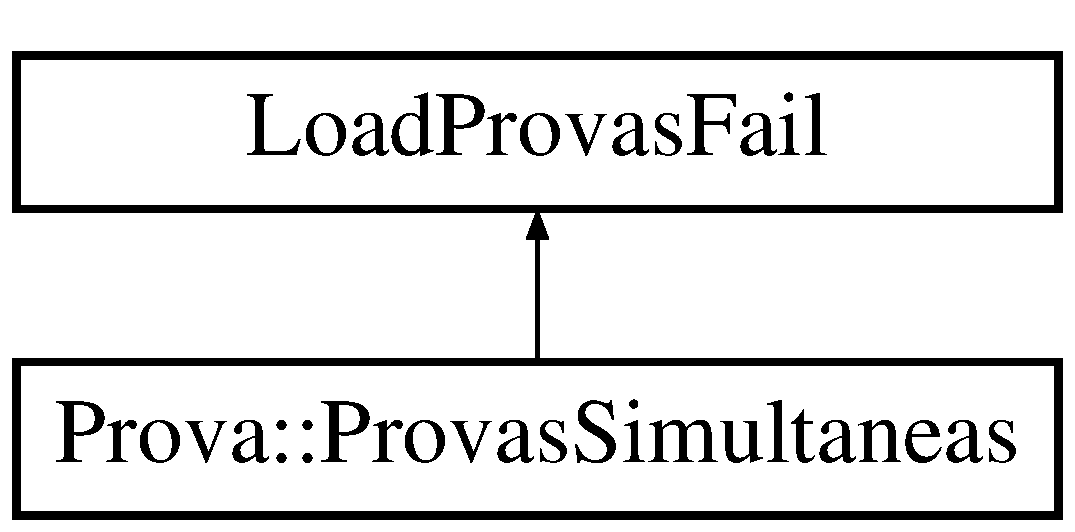
\includegraphics[height=2.000000cm]{class_prova_1_1_provas_simultaneas}
\end{center}
\end{figure}
\subsection*{Public Member Functions}
\begin{DoxyCompactItemize}
\item 
\hyperlink{class_prova_1_1_provas_simultaneas_a4cee5b7ff5cfcee9db81e5075b1d9070}{Provas\+Simultaneas} (string m1, string m2)
\item 
string \hyperlink{class_prova_1_1_provas_simultaneas_a57bf315de1374fd819951fea3fcd129b}{get\+Message} () const 
\end{DoxyCompactItemize}


\subsection{Detailed Description}
Uma expecao para quando duas provas sao incompativeis 

\subsection{Constructor \& Destructor Documentation}
\hypertarget{class_prova_1_1_provas_simultaneas_a4cee5b7ff5cfcee9db81e5075b1d9070}{}\index{Prova\+::\+Provas\+Simultaneas@{Prova\+::\+Provas\+Simultaneas}!Provas\+Simultaneas@{Provas\+Simultaneas}}
\index{Provas\+Simultaneas@{Provas\+Simultaneas}!Prova\+::\+Provas\+Simultaneas@{Prova\+::\+Provas\+Simultaneas}}
\subsubsection[{Provas\+Simultaneas(string m1, string m2)}]{\setlength{\rightskip}{0pt plus 5cm}Prova\+::\+Provas\+Simultaneas\+::\+Provas\+Simultaneas (
\begin{DoxyParamCaption}
\item[{string}]{m1, }
\item[{string}]{m2}
\end{DoxyParamCaption}
)\hspace{0.3cm}{\ttfamily [inline]}}\label{class_prova_1_1_provas_simultaneas_a4cee5b7ff5cfcee9db81e5075b1d9070}

\begin{DoxyParams}{Parameters}
{\em m1} & -\/ modalidade \\
\hline
{\em m2} & -\/ outra modalidade \\
\hline
\end{DoxyParams}


\subsection{Member Function Documentation}
\hypertarget{class_prova_1_1_provas_simultaneas_a57bf315de1374fd819951fea3fcd129b}{}\index{Prova\+::\+Provas\+Simultaneas@{Prova\+::\+Provas\+Simultaneas}!get\+Message@{get\+Message}}
\index{get\+Message@{get\+Message}!Prova\+::\+Provas\+Simultaneas@{Prova\+::\+Provas\+Simultaneas}}
\subsubsection[{get\+Message() const }]{\setlength{\rightskip}{0pt plus 5cm}string Prova\+::\+Provas\+Simultaneas\+::get\+Message (
\begin{DoxyParamCaption}
{}
\end{DoxyParamCaption}
) const\hspace{0.3cm}{\ttfamily [inline]}, {\ttfamily [virtual]}}\label{class_prova_1_1_provas_simultaneas_a57bf315de1374fd819951fea3fcd129b}
cria uma mensagem com os nomes de m1 e m2 \begin{DoxyReturn}{Returns}
uma mensagem de erro 
\end{DoxyReturn}


Implements \hyperlink{class_load_provas_fail}{Load\+Provas\+Fail}.



The documentation for this class was generated from the following file\+:\begin{DoxyCompactItemize}
\item 
src/Prova.\+h\end{DoxyCompactItemize}

\hypertarget{class_prova_terminada}{}\section{Prova\+Terminada Class Reference}
\label{class_prova_terminada}\index{Prova\+Terminada@{Prova\+Terminada}}


{\ttfamily \#include $<$Prova.\+h$>$}

Inheritance diagram for Prova\+Terminada\+:\begin{figure}[H]
\begin{center}
\leavevmode
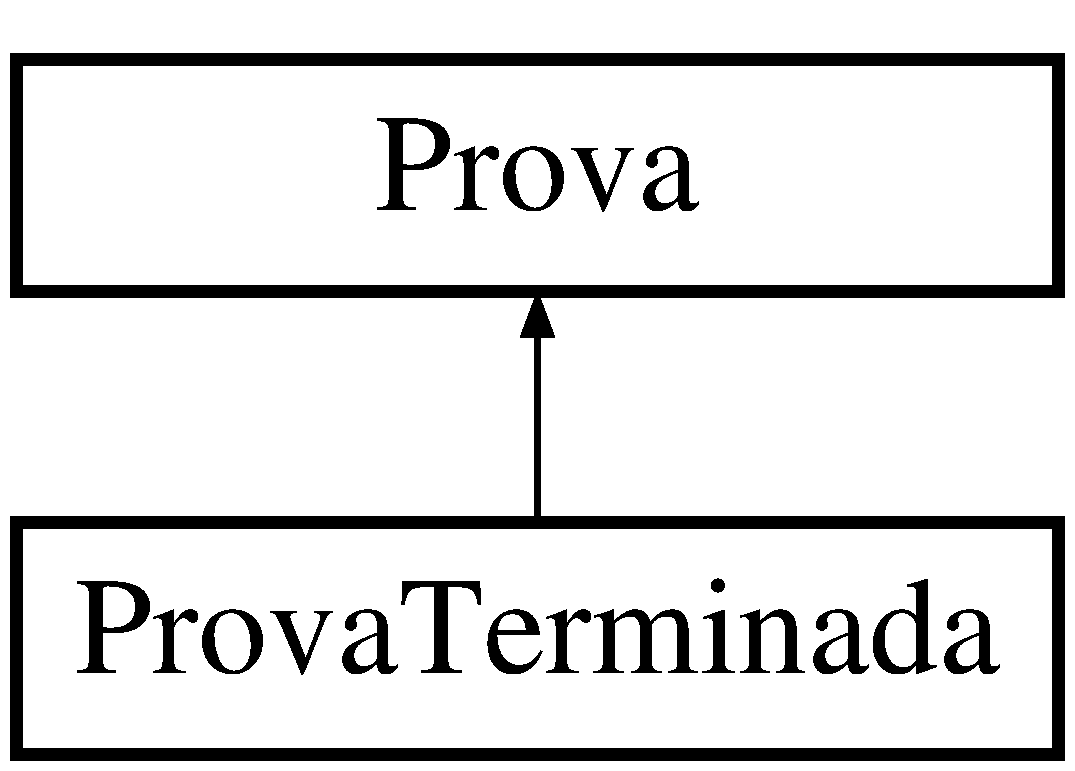
\includegraphics[height=2.000000cm]{class_prova_terminada}
\end{center}
\end{figure}
\subsection*{Public Member Functions}
\begin{DoxyCompactItemize}
\item 
\hyperlink{class_prova_terminada_a273ba377768056d52dc71770d91c860c}{Prova\+Terminada} (\hyperlink{class_modalidade}{Modalidade} $\ast$m, \hyperlink{class_data}{Data} d, \hyperlink{class_hora}{Hora} i, char g)
\item 
\hyperlink{class_atleta}{Atleta} $\ast$ \hyperlink{class_prova_terminada_aa66bb50f4a969d6a4795bb39595705d8}{get\+Primeiro} () const 
\item 
\hyperlink{class_atleta}{Atleta} $\ast$ \hyperlink{class_prova_terminada_a3117799dd3ddb513442376203f0ea035}{get\+Segundo} () const 
\item 
\hyperlink{class_atleta}{Atleta} $\ast$ \hyperlink{class_prova_terminada_a332c8f4466c18f153a3ebf7347ab944a}{get\+Terceiro} () const 
\item 
vector$<$ float $>$ \hyperlink{class_prova_terminada_a449d07fa099785eda45301303792b6b0}{get\+Pontuacoes} () const 
\item 
void \hyperlink{class_prova_terminada_a189ef4830e8e6dbe3e50153bdc28b1ed}{set\+Atletas} (vector$<$ \hyperlink{class_atleta}{Atleta} $\ast$ $>$ a)
\item 
\hypertarget{class_prova_terminada_a8b02034c7190ad01ee7674d166595c97}{}void {\bfseries set\+Pontuacoes} (vector$<$ float $>$ pont)\label{class_prova_terminada_a8b02034c7190ad01ee7674d166595c97}

\item 
\hypertarget{class_prova_terminada_afcff2f98ae33bf903ee3bee4c2a47f37}{}void {\bfseries set\+Pontuacoes\+Atletas} (vector$<$ pair$<$ \hyperlink{class_atleta}{Atleta} $\ast$, float $>$ $>$)\label{class_prova_terminada_afcff2f98ae33bf903ee3bee4c2a47f37}

\item 
\hypertarget{class_prova_terminada_a9a5ce1362cea1c8aba698c1b7a71d2e2}{}void {\bfseries set\+Pontuacoes\+Atletas\+Rev} (vector$<$ pair$<$ \hyperlink{class_atleta}{Atleta} $\ast$, float $>$ $>$)\label{class_prova_terminada_a9a5ce1362cea1c8aba698c1b7a71d2e2}

\item 
bool \hyperlink{class_prova_terminada_afe024233747b571f92080b6fc325b6a5}{operator$<$} (const \hyperlink{class_prova_terminada}{Prova\+Terminada} \&p) const 
\end{DoxyCompactItemize}
\subsection*{Additional Inherited Members}


\subsection{Detailed Description}
class \hyperlink{class_prova_terminada}{Prova\+Terminada}

Representa uma prova que ja ocorreu 

\subsection{Constructor \& Destructor Documentation}
\hypertarget{class_prova_terminada_a273ba377768056d52dc71770d91c860c}{}\index{Prova\+Terminada@{Prova\+Terminada}!Prova\+Terminada@{Prova\+Terminada}}
\index{Prova\+Terminada@{Prova\+Terminada}!Prova\+Terminada@{Prova\+Terminada}}
\subsubsection[{Prova\+Terminada(\+Modalidade $\ast$m, Data d, Hora i, char g)}]{\setlength{\rightskip}{0pt plus 5cm}Prova\+Terminada\+::\+Prova\+Terminada (
\begin{DoxyParamCaption}
\item[{{\bf Modalidade} $\ast$}]{m, }
\item[{{\bf Data}}]{d, }
\item[{{\bf Hora}}]{i, }
\item[{char}]{g}
\end{DoxyParamCaption}
)}\label{class_prova_terminada_a273ba377768056d52dc71770d91c860c}

\begin{DoxyParams}{Parameters}
{\em m} & -\/ modalidade \\
\hline
{\em d} & -\/ data \\
\hline
{\em i} & -\/ hora \\
\hline
{\em g} & -\/ genero \\
\hline
\end{DoxyParams}


\subsection{Member Function Documentation}
\hypertarget{class_prova_terminada_a449d07fa099785eda45301303792b6b0}{}\index{Prova\+Terminada@{Prova\+Terminada}!get\+Pontuacoes@{get\+Pontuacoes}}
\index{get\+Pontuacoes@{get\+Pontuacoes}!Prova\+Terminada@{Prova\+Terminada}}
\subsubsection[{get\+Pontuacoes() const }]{\setlength{\rightskip}{0pt plus 5cm}vector$<$ float $>$ Prova\+Terminada\+::get\+Pontuacoes (
\begin{DoxyParamCaption}
{}
\end{DoxyParamCaption}
) const}\label{class_prova_terminada_a449d07fa099785eda45301303792b6b0}
\begin{DoxyReturn}{Returns}
pontuacoes 
\end{DoxyReturn}
\hypertarget{class_prova_terminada_aa66bb50f4a969d6a4795bb39595705d8}{}\index{Prova\+Terminada@{Prova\+Terminada}!get\+Primeiro@{get\+Primeiro}}
\index{get\+Primeiro@{get\+Primeiro}!Prova\+Terminada@{Prova\+Terminada}}
\subsubsection[{get\+Primeiro() const }]{\setlength{\rightskip}{0pt plus 5cm}{\bf Atleta} $\ast$ Prova\+Terminada\+::get\+Primeiro (
\begin{DoxyParamCaption}
{}
\end{DoxyParamCaption}
) const\hspace{0.3cm}{\ttfamily [virtual]}}\label{class_prova_terminada_aa66bb50f4a969d6a4795bb39595705d8}
\begin{DoxyReturn}{Returns}
o atleta em primeiro lugar 
\end{DoxyReturn}


Reimplemented from \hyperlink{class_prova}{Prova}.

\hypertarget{class_prova_terminada_a3117799dd3ddb513442376203f0ea035}{}\index{Prova\+Terminada@{Prova\+Terminada}!get\+Segundo@{get\+Segundo}}
\index{get\+Segundo@{get\+Segundo}!Prova\+Terminada@{Prova\+Terminada}}
\subsubsection[{get\+Segundo() const }]{\setlength{\rightskip}{0pt plus 5cm}{\bf Atleta} $\ast$ Prova\+Terminada\+::get\+Segundo (
\begin{DoxyParamCaption}
{}
\end{DoxyParamCaption}
) const}\label{class_prova_terminada_a3117799dd3ddb513442376203f0ea035}
\begin{DoxyReturn}{Returns}
o atleta em segundo lugar 
\end{DoxyReturn}
\hypertarget{class_prova_terminada_a332c8f4466c18f153a3ebf7347ab944a}{}\index{Prova\+Terminada@{Prova\+Terminada}!get\+Terceiro@{get\+Terceiro}}
\index{get\+Terceiro@{get\+Terceiro}!Prova\+Terminada@{Prova\+Terminada}}
\subsubsection[{get\+Terceiro() const }]{\setlength{\rightskip}{0pt plus 5cm}{\bf Atleta} $\ast$ Prova\+Terminada\+::get\+Terceiro (
\begin{DoxyParamCaption}
{}
\end{DoxyParamCaption}
) const\hspace{0.3cm}{\ttfamily [virtual]}}\label{class_prova_terminada_a332c8f4466c18f153a3ebf7347ab944a}
\begin{DoxyReturn}{Returns}
o atleta em terceiro lugar 
\end{DoxyReturn}


Reimplemented from \hyperlink{class_prova}{Prova}.

\hypertarget{class_prova_terminada_afe024233747b571f92080b6fc325b6a5}{}\index{Prova\+Terminada@{Prova\+Terminada}!operator$<$@{operator$<$}}
\index{operator$<$@{operator$<$}!Prova\+Terminada@{Prova\+Terminada}}
\subsubsection[{operator$<$(const Prova\+Terminada \&p) const }]{\setlength{\rightskip}{0pt plus 5cm}bool Prova\+Terminada\+::operator$<$ (
\begin{DoxyParamCaption}
\item[{const {\bf Prova\+Terminada} \&}]{p}
\end{DoxyParamCaption}
) const}\label{class_prova_terminada_afe024233747b571f92080b6fc325b6a5}

\begin{DoxyParams}{Parameters}
{\em p2} & -\/ prova \\
\hline
\end{DoxyParams}
\begin{DoxyReturn}{Returns}
true se occorer antes p2, false se nao 
\end{DoxyReturn}
\hypertarget{class_prova_terminada_a189ef4830e8e6dbe3e50153bdc28b1ed}{}\index{Prova\+Terminada@{Prova\+Terminada}!set\+Atletas@{set\+Atletas}}
\index{set\+Atletas@{set\+Atletas}!Prova\+Terminada@{Prova\+Terminada}}
\subsubsection[{set\+Atletas(vector$<$ Atleta $\ast$ $>$ a)}]{\setlength{\rightskip}{0pt plus 5cm}void Prova\+Terminada\+::set\+Atletas (
\begin{DoxyParamCaption}
\item[{vector$<$ {\bf Atleta} $\ast$ $>$}]{a}
\end{DoxyParamCaption}
)}\label{class_prova_terminada_a189ef4830e8e6dbe3e50153bdc28b1ed}
Muda atletas para a; 
\begin{DoxyParams}{Parameters}
{\em a} & -\/ um vetor de atletas \\
\hline
\end{DoxyParams}


The documentation for this class was generated from the following files\+:\begin{DoxyCompactItemize}
\item 
src/Prova.\+h\item 
src/Prova.\+cpp\end{DoxyCompactItemize}

%--- End generated contents ---

% Index
\backmatter
\newpage
\phantomsection
\clearemptydoublepage
\addcontentsline{toc}{chapter}{Index}
\printindex

\end{document}
